\documentclass[twoside]{book}

% Packages required by doxygen
\usepackage{fixltx2e}
\usepackage{calc}
\usepackage{doxygen}
\usepackage[export]{adjustbox} % also loads graphicx
\usepackage{graphicx}
\usepackage[utf8]{inputenc}
\usepackage{makeidx}
\usepackage{multicol}
\usepackage{multirow}
\PassOptionsToPackage{warn}{textcomp}
\usepackage{textcomp}
\usepackage[nointegrals]{wasysym}
\usepackage[table]{xcolor}

% NLS support packages
\usepackage[spanish]{babel}
% Font selection
\usepackage[T1]{fontenc}
\usepackage[scaled=.90]{helvet}
\usepackage{courier}
\usepackage{amssymb}
\usepackage{sectsty}
\renewcommand{\familydefault}{\sfdefault}
\allsectionsfont{%
  \fontseries{bc}\selectfont%
  \color{darkgray}%
}
\renewcommand{\DoxyLabelFont}{%
  \fontseries{bc}\selectfont%
  \color{darkgray}%
}
\newcommand{\+}{\discretionary{\mbox{\scriptsize$\hookleftarrow$}}{}{}}

% Page & text layout
\usepackage{geometry}
\geometry{%
  a4paper,%
  top=2.5cm,%
  bottom=2.5cm,%
  left=2.5cm,%
  right=2.5cm%
}
\tolerance=750
\hfuzz=15pt
\hbadness=750
\setlength{\emergencystretch}{15pt}
\setlength{\parindent}{0cm}
\setlength{\parskip}{0.2cm}
\makeatletter
\renewcommand{\paragraph}{%
  \@startsection{paragraph}{4}{0ex}{-1.0ex}{1.0ex}{%
    \normalfont\normalsize\bfseries\SS@parafont%
  }%
}
\renewcommand{\subparagraph}{%
  \@startsection{subparagraph}{5}{0ex}{-1.0ex}{1.0ex}{%
    \normalfont\normalsize\bfseries\SS@subparafont%
  }%
}
\makeatother

% Headers & footers
\usepackage{fancyhdr}
\pagestyle{fancyplain}
\fancyhead[LE]{\fancyplain{}{\bfseries\thepage}}
\fancyhead[CE]{\fancyplain{}{}}
\fancyhead[RE]{\fancyplain{}{\bfseries\leftmark}}
\fancyhead[LO]{\fancyplain{}{\bfseries\rightmark}}
\fancyhead[CO]{\fancyplain{}{}}
\fancyhead[RO]{\fancyplain{}{\bfseries\thepage}}
\fancyfoot[LE]{\fancyplain{}{}}
\fancyfoot[CE]{\fancyplain{}{}}
\fancyfoot[RE]{\fancyplain{}{\bfseries\scriptsize Generado el Lunes, 13 de Marzo de 2017 00\+:11\+:50 para Redes de Comunicaciones I\+I por Doxygen }}
\fancyfoot[LO]{\fancyplain{}{\bfseries\scriptsize Generado el Lunes, 13 de Marzo de 2017 00\+:11\+:50 para Redes de Comunicaciones I\+I por Doxygen }}
\fancyfoot[CO]{\fancyplain{}{}}
\fancyfoot[RO]{\fancyplain{}{}}
\renewcommand{\footrulewidth}{0.4pt}
\renewcommand{\chaptermark}[1]{%
  \markboth{#1}{}%
}
\renewcommand{\sectionmark}[1]{%
  \markright{\thesection\ #1}%
}

% Indices & bibliography
\usepackage{natbib}
\usepackage[titles]{tocloft}
\setcounter{tocdepth}{3}
\setcounter{secnumdepth}{5}
\makeindex

% Hyperlinks (required, but should be loaded last)
\usepackage{ifpdf}
\ifpdf
  \usepackage[pdftex,pagebackref=true]{hyperref}
\else
  \usepackage[ps2pdf,pagebackref=true]{hyperref}
\fi
\hypersetup{%
  colorlinks=true,%
  linkcolor=blue,%
  citecolor=blue,%
  unicode%
}

% Custom commands
\newcommand{\clearemptydoublepage}{%
  \newpage{\pagestyle{empty}\cleardoublepage}%
}


%===== C O N T E N T S =====

\begin{document}

% Titlepage & ToC
\hypersetup{pageanchor=false,
             bookmarks=true,
             bookmarksnumbered=true,
             pdfencoding=unicode
            }
\pagenumbering{roman}
\begin{titlepage}
\vspace*{7cm}
\begin{center}%
{\Large Redes de Comunicaciones I\+I \\[1ex]\large 1.\+0 }\\
\vspace*{1cm}
{\large Generado por Doxygen 1.8.9.1}\\
\vspace*{0.5cm}
{\small Lunes, 13 de Marzo de 2017 00:11:50}\\
\end{center}
\end{titlepage}
\clearemptydoublepage
\tableofcontents
\clearemptydoublepage
\pagenumbering{arabic}
\hypersetup{pageanchor=true}

%--- Begin generated contents ---
\chapter{P1 -\/ Servidor I\+R\+C}
\label{index}\hypertarget{index}{}En esta página se encuentra disponible la documentación de librería S\+SL de la práctica 3 de Redes de Comunicaciones II, grupo 2313, pareja 6.

\section*{Librería S\+SL}

La librería S\+SL proporciona una capa superior a las funciones de los servidores echo proporcionados para la práctica. En ella se encuentran las funciones de fijación, conexión, envío y recepción mediante la capa S\+SL de socket. 
\begin{DoxyItemize}
\item \hyperlink{inicializar_nivel_SSL}{Inicialización de S\+SL} 
\item \hyperlink{fijar_contexto_SSL}{Fijación del contexto S\+SL} 
\item \hyperlink{aceptar_canal_seguro_SSL}{Aceptación de un canal seguro} 
\item \hyperlink{evaluar_post_connectar_SSL}{Comprobación de conexión S\+SL} 
\item \hyperlink{enviar_datos_SSL}{Envío de datos vía S\+SL} 
\item \hyperlink{recibir_datos_SSL}{Recepción de datos vía S\+SL} 
\item \hyperlink{cerrar_canal_SSL}{Cierre de un canal S\+SL} 
\item \hyperlink{conectar_canal_seguro_SSL}{Conexión a un canal S\+SL} 
\end{DoxyItemize}
\begin{DoxyImageNoCaption}
  \mbox{\includegraphics[width=\textwidth,height=\textheight/2,keepaspectratio=true]{dot_}}
\end{DoxyImageNoCaption}
 
\chapter{Funciones auxiliares}
\label{server_common_functions}
\hypertarget{server_common_functions}{}
Esta sección incluye las funciones auxiliares utilizadas por los comandos para obtener datos de los usuarios como por ejemplo el nick, username, etc. Además incluye funciones para buscar coincidencias por un descriptor del socket de un cliente o si un canal existe con un nombre dado.\hypertarget{server_common_functions_cabeceras2}{}\section{Cabeceras}\label{server_common_functions_cabeceras2}
{\ttfamily  {\bfseries \#include} {\bfseries $<$\hyperlink{G-2313-06-P1__common__functions_8h}{G-\/2313-\/06-\/\+P1\+\_\+common\+\_\+functions.\+h}$>$} } \hypertarget{server_common_functions_functions2}{}\section{Funciones implementadas}\label{server_common_functions_functions2}
Se incluyen las siguientes funciones\+: 
\begin{DoxyItemize}
\item \hyperlink{server_users_find_by_nick}{server\+\_\+users\+\_\+find\+\_\+by\+\_\+nick} 
\item \hyperlink{server_users_find_by_socket}{server\+\_\+users\+\_\+find\+\_\+by\+\_\+socket} 
\item \hyperlink{server_channels_find_by_name}{server\+\_\+channels\+\_\+find\+\_\+by\+\_\+name} 
\item \hyperlink{server_channels_update_nick}{server\+\_\+channels\+\_\+update\+\_\+nick} 
\item \hyperlink{server_channels_update_away}{server\+\_\+channels\+\_\+update\+\_\+away} 
\item \hyperlink{server_return_user}{server\+\_\+return\+\_\+user} 
\end{DoxyItemize}\hypertarget{server_users_find_by_nick}{}\section{server\+\_\+users\+\_\+find\+\_\+by\+\_\+nick}\label{server_users_find_by_nick}
Busca un usuario por un nick dado.\hypertarget{server_users_find_by_nick_synopsis_server_users_find_by_nick}{}\subsection{Synopsis}\label{server_users_find_by_nick_synopsis_server_users_find_by_nick}
{\ttfamily  {\bfseries \#include} {\bfseries $<$\hyperlink{G-2313-06-P1__common__functions_8h}{G-\/2313-\/06-\/\+P1\+\_\+common\+\_\+functions.\+h}$>$} ~\newline
 {\bfseries int \hyperlink{G-2313-06-P1__common__functions_8c_a61cca6f1a1adeb81f722ecc2ff35aab5}{server\+\_\+users\+\_\+find\+\_\+by\+\_\+nick(char$\ast$ data)}} } \hypertarget{server_users_find_by_nick_descripcion_server_users_find_by_nick}{}\subsection{Descripción}\label{server_users_find_by_nick_descripcion_server_users_find_by_nick}
Utiliza la función {\bfseries I\+R\+C\+T\+A\+D\+User\+\_\+\+Get\+Data} del T\+A\+D para buscar un usuario que cumpla las características de nick recibidas como parámetro {\bfseries char $\ast$data}. Devuelve un valor booleano.\hypertarget{server_users_find_by_nick_return_server_users_find_by_nick}{}\subsection{Valores devueltos}\label{server_users_find_by_nick_return_server_users_find_by_nick}

\begin{DoxyItemize}
\item {\bfseries int} Devuelve valor verdado/falso dependiendo de la búsqueda. 
\end{DoxyItemize}\hypertarget{server_users_find_by_nick_authors_server_users_find_by_nick}{}\subsection{Autores}\label{server_users_find_by_nick_authors_server_users_find_by_nick}

\begin{DoxyItemize}
\item Jorge Parrilla Llamas (\href{mailto:jorge.parrilla@estudiante.uam.es}{\tt jorge.\+parrilla@estudiante.\+uam.\+es}) 
\item Javier de Marco Tomás (\href{mailto:javier.marco@estudiante.uam.es}{\tt javier.\+marco@estudiante.\+uam.\+es}) 
\end{DoxyItemize}\hypertarget{server_users_find_by_socket}{}\section{server\+\_\+users\+\_\+find\+\_\+by\+\_\+socket}\label{server_users_find_by_socket}
Busca un usuario por un socket dado.\hypertarget{server_users_find_by_socket_synopsis_server_users_find_by_socket}{}\subsection{Synopsis}\label{server_users_find_by_socket_synopsis_server_users_find_by_socket}
{\ttfamily  {\bfseries \#include} {\bfseries $<$\hyperlink{G-2313-06-P1__common__functions_8h}{G-\/2313-\/06-\/\+P1\+\_\+common\+\_\+functions.\+h}$>$} ~\newline
 {\bfseries int \hyperlink{G-2313-06-P1__common__functions_8c_a485e68f66db6ae4b7297d99c32afe30a}{server\+\_\+users\+\_\+find\+\_\+by\+\_\+socket(int sockdesc)}} } \hypertarget{server_users_find_by_socket_descripcion_server_users_find_by_socket}{}\subsection{Descripción}\label{server_users_find_by_socket_descripcion_server_users_find_by_socket}
Utiliza la función {\bfseries I\+R\+C\+T\+A\+D\+User\+\_\+\+Get\+Data} del T\+A\+D para buscar un usuario que cumpla las características de socket recibidas como parámetro {\bfseries int sockdesc}.\hypertarget{server_users_find_by_socket_return_server_users_find_by_socket}{}\subsection{Valores devueltos}\label{server_users_find_by_socket_return_server_users_find_by_socket}

\begin{DoxyItemize}
\item {\bfseries int} Devuelve valor verdado/falso dependiendo de la búsqueda. 
\end{DoxyItemize}\hypertarget{server_users_find_by_socket_authors_server_users_find_by_socket}{}\subsection{Autores}\label{server_users_find_by_socket_authors_server_users_find_by_socket}

\begin{DoxyItemize}
\item Jorge Parrilla Llamas (\href{mailto:jorge.parrilla@estudiante.uam.es}{\tt jorge.\+parrilla@estudiante.\+uam.\+es}) 
\item Javier de Marco Tomás (\href{mailto:javier.marco@estudiante.uam.es}{\tt javier.\+marco@estudiante.\+uam.\+es}) 
\end{DoxyItemize}\hypertarget{server_channels_find_by_name}{}\section{server\+\_\+channels\+\_\+find\+\_\+by\+\_\+name}\label{server_channels_find_by_name}
Busca un canal por un nombre dado.\hypertarget{server_channels_find_by_name_synopsis_server_users_find_by_name}{}\subsection{Synopsis}\label{server_channels_find_by_name_synopsis_server_users_find_by_name}
{\ttfamily  {\bfseries \#include} {\bfseries $<$\hyperlink{G-2313-06-P1__common__functions_8h}{G-\/2313-\/06-\/\+P1\+\_\+common\+\_\+functions.\+h}$>$} ~\newline
 {\bfseries int \hyperlink{G-2313-06-P1__common__functions_8c_a875ae5278d95716b494b26f96cf4ae6e}{server\+\_\+channels\+\_\+find\+\_\+by\+\_\+name(char $\ast$channel)}} } \hypertarget{server_channels_find_by_name_descripcion_server_channels_find_by_name}{}\subsection{Descripción}\label{server_channels_find_by_name_descripcion_server_channels_find_by_name}
Utiliza la función {\bfseries I\+R\+C\+T\+A\+D\+User\+\_\+\+Get\+Data} del T\+A\+D para buscar un canal que cumpla las características de nombre recibidas como parámetro {\bfseries char $\ast$channel}.\hypertarget{server_channels_find_by_name_return_server_channels_find_by_name}{}\subsection{Valores devueltos}\label{server_channels_find_by_name_return_server_channels_find_by_name}

\begin{DoxyItemize}
\item {\bfseries int} Devuelve valor verdado/falso dependiendo de la búsqueda. 
\end{DoxyItemize}\hypertarget{server_channels_find_by_name_authors_server_channels_find_by_name}{}\subsection{Autores}\label{server_channels_find_by_name_authors_server_channels_find_by_name}

\begin{DoxyItemize}
\item Jorge Parrilla Llamas (\href{mailto:jorge.parrilla@estudiante.uam.es}{\tt jorge.\+parrilla@estudiante.\+uam.\+es}) 
\item Javier de Marco Tomás (\href{mailto:javier.marco@estudiante.uam.es}{\tt javier.\+marco@estudiante.\+uam.\+es}) 
\end{DoxyItemize}\hypertarget{server_channels_update_nick}{}\section{server\+\_\+channels\+\_\+update\+\_\+nick}\label{server_channels_update_nick}
Actualiza el nick de un usuario.\hypertarget{server_channels_update_nick_synopsis_server_channels_update_nick}{}\subsection{Synopsis}\label{server_channels_update_nick_synopsis_server_channels_update_nick}
{\ttfamily  {\bfseries \#include} {\bfseries $<$\hyperlink{G-2313-06-P1__common__functions_8h}{G-\/2313-\/06-\/\+P1\+\_\+common\+\_\+functions.\+h}$>$} ~\newline
 {\bfseries int server\+\_\+channels\+\_\+update\+\_\+nick(char {\itshape nick\+\_\+old, char} nick\+\_\+new)} } \hypertarget{server_channels_update_nick_descripcion_server_channels_update_nick}{}\subsection{Descripción}\label{server_channels_update_nick_descripcion_server_channels_update_nick}
Actualiza el nick de un usuario mediante la función del T\+A\+D {\bfseries I\+R\+C\+T\+A\+D\+User\+\_\+\+Set} para actualizar datos de los usuarios. 

Comprueba previamente que el usuario exista mediante la función {\bfseries I\+R\+C\+T\+A\+D\+User\+\_\+\+Get\+Data} utilizando los parámetros recibidos {\bfseries char $\ast$nick\+\_\+old} y {\bfseries char $\ast$nick\+\_\+new}.\hypertarget{server_channels_update_nick_return_server_channels_update_nick}{}\subsection{Valores devueltos}\label{server_channels_update_nick_return_server_channels_update_nick}

\begin{DoxyItemize}
\item {\bfseries int} Devuelve valor verdado/falso dependiendo de la búsqueda. 
\end{DoxyItemize}\hypertarget{server_channels_update_nick_authors_server_channels_update_nick}{}\subsection{Autores}\label{server_channels_update_nick_authors_server_channels_update_nick}

\begin{DoxyItemize}
\item Jorge Parrilla Llamas (\href{mailto:jorge.parrilla@estudiante.uam.es}{\tt jorge.\+parrilla@estudiante.\+uam.\+es}) 
\item Javier de Marco Tomás (\href{mailto:javier.marco@estudiante.uam.es}{\tt javier.\+marco@estudiante.\+uam.\+es}) 
\end{DoxyItemize}\hypertarget{server_channels_update_away}{}\section{server\+\_\+channels\+\_\+update\+\_\+away}\label{server_channels_update_away}
Actualiza el mensaje away de un usuario.\hypertarget{server_channels_update_away_synopsis_server_channels_update_away}{}\subsection{Synopsis}\label{server_channels_update_away_synopsis_server_channels_update_away}
{\ttfamily  {\bfseries \#include} {\bfseries $<$\hyperlink{G-2313-06-P1__common__functions_8h}{G-\/2313-\/06-\/\+P1\+\_\+common\+\_\+functions.\+h}$>$} ~\newline
 {\bfseries int \hyperlink{G-2313-06-P1__common__functions_8c_af9aeb632d55a4cbbe842ab97001b5128}{server\+\_\+channels\+\_\+update\+\_\+away(char$\ast$ nick, char$\ast$ away)}} } \hypertarget{server_channels_update_away_descripcion_server_channels_update_away}{}\subsection{Descripción}\label{server_channels_update_away_descripcion_server_channels_update_away}
Actualiza el mensaje away de un usuario mediante la función del T\+A\+D {\bfseries I\+R\+C\+T\+A\+D\+User\+\_\+\+Set\+Away} para actualizar los away de los usuarios mediante el parámetro recibido {\bfseries char $\ast$away}. 

Comprueba previamente que el usuario exista mediante la función {\bfseries I\+R\+C\+T\+A\+D\+User\+\_\+\+Get\+Data} utilizando el parámetro recibido {\bfseries char $\ast$nick}.\hypertarget{server_channels_update_away_return_server_channels_update_away}{}\subsection{Valores devueltos}\label{server_channels_update_away_return_server_channels_update_away}

\begin{DoxyItemize}
\item {\bfseries int} Devuelve valor verdado/falso dependiendo de la búsqueda. 
\end{DoxyItemize}\hypertarget{server_channels_update_away_authors_server_channels_update_away}{}\subsection{Autores}\label{server_channels_update_away_authors_server_channels_update_away}

\begin{DoxyItemize}
\item Jorge Parrilla Llamas (\href{mailto:jorge.parrilla@estudiante.uam.es}{\tt jorge.\+parrilla@estudiante.\+uam.\+es}) 
\item Javier de Marco Tomás (\href{mailto:javier.marco@estudiante.uam.es}{\tt javier.\+marco@estudiante.\+uam.\+es}) 
\end{DoxyItemize}\hypertarget{server_return_user}{}\section{server\+\_\+return\+\_\+user}\label{server_return_user}
Devuelve el username de un usuario.\hypertarget{server_return_user_synopsis_server_return_user}{}\subsection{Synopsis}\label{server_return_user_synopsis_server_return_user}
{\ttfamily  {\bfseries \#include} {\bfseries $<$\hyperlink{G-2313-06-P1__common__functions_8h}{G-\/2313-\/06-\/\+P1\+\_\+common\+\_\+functions.\+h}$>$} ~\newline
 {\bfseries char$\ast$ \hyperlink{G-2313-06-P1__common__functions_8c_a230bf24ab7ae18d2e81ebc1d3575a6ad}{server\+\_\+return\+\_\+user(char$\ast$ nick)}} } \hypertarget{server_return_user_descripcion_server_return_user}{}\subsection{Descripción}\label{server_return_user_descripcion_server_return_user}
Devuelve el username de un usuario utilizando la función del T\+A\+D {\bfseries I\+R\+C\+T\+A\+D\+User\+\_\+\+Get\+Data} para obtener información de los usuarios mediante el parámetro recibido {\bfseries char $\ast$nick}. \hypertarget{server_return_user_return_server_return_user}{}\subsection{Valores devueltos}\label{server_return_user_return_server_return_user}

\begin{DoxyItemize}
\item {\bfseries char$\ast$} Devuelve un puntero al username del usuario. 
\end{DoxyItemize}\hypertarget{server_return_user_authors_server_return_user}{}\subsection{Autores}\label{server_return_user_authors_server_return_user}

\begin{DoxyItemize}
\item Jorge Parrilla Llamas (\href{mailto:jorge.parrilla@estudiante.uam.es}{\tt jorge.\+parrilla@estudiante.\+uam.\+es}) 
\item Javier de Marco Tomás (\href{mailto:javier.marco@estudiante.uam.es}{\tt javier.\+marco@estudiante.\+uam.\+es}) 
\end{DoxyItemize}
\chapter{Comandos}
\label{server_commands}
\hypertarget{server_commands}{}
Esta sección incluye las funciones de comandos utilizadas para parsear los comandos recibidos del I\+RC. A estas funciones accede el array de punteros a función descrito en {\bfseries server\+\_\+execute\+\_\+function}.\hypertarget{server_commands_cabeceras3}{}\section{Cabeceras}\label{server_commands_cabeceras3}
{\ttfamily  {\bfseries \#include} {\bfseries $<$G-\/2313-\/06-\/\+P1\+\_\+function\+\_\+handlers.\+h.\+h$>$} } \hypertarget{server_commands_functions3}{}\section{Funciones implementadas}\label{server_commands_functions3}
Se incluyen las siguientes funciones\+: 
\begin{DoxyItemize}
\item \hyperlink{server_command_nick}{server\+\_\+command\+\_\+nick} 
\item \hyperlink{server_command_user}{server\+\_\+command\+\_\+user} 
\item \hyperlink{server_command_join}{server\+\_\+command\+\_\+join} 
\item \hyperlink{server_command_quit}{server\+\_\+command\+\_\+quit} 
\item \hyperlink{server_command_ping}{server\+\_\+command\+\_\+ping} 
\item \hyperlink{server_command_list}{server\+\_\+command\+\_\+list} 
\item \hyperlink{server_command_privmsg}{server\+\_\+command\+\_\+privmsg} 
\item \hyperlink{server_command_part}{server\+\_\+command\+\_\+part} 
\item \hyperlink{server_command_names}{server\+\_\+command\+\_\+names} 
\item \hyperlink{server_command_kick}{server\+\_\+command\+\_\+kick} 
\item \hyperlink{server_command_mode}{server\+\_\+command\+\_\+mode} 
\item \hyperlink{server_command_away}{server\+\_\+command\+\_\+away} 
\item \hyperlink{server_command_whois}{server\+\_\+command\+\_\+whois} 
\item \hyperlink{server_command_topic}{server\+\_\+command\+\_\+topic} 
\item \hyperlink{server_command_motd}{server\+\_\+command\+\_\+motd} 
\end{DoxyItemize}\hypertarget{server_command_nick}{}\section{server\+\_\+command\+\_\+nick}\label{server_command_nick}
Función handler del comando N\+I\+CK del I\+RC.\hypertarget{server_command_nick_synopsis_nick}{}\subsection{Synopsis}\label{server_command_nick_synopsis_nick}
{\ttfamily  {\bfseries \#include} {\bfseries $<$\hyperlink{G-2313-06-P1__function__handlers_8h}{G-\/2313-\/06-\/\+P1\+\_\+function\+\_\+handlers.\+h}$>$} ~\newline
 {\bfseries void \hyperlink{G-2313-06-P1__function__handlers_8c_aeefab469ba48ce1655dd5afd14f104b4}{server\+\_\+command\+\_\+nick(char$\ast$ command, int desc, char $\ast$ nick\+\_\+static, int$\ast$ register\+\_\+status)}} } \hypertarget{server_command_nick_descripcion_nick}{}\subsection{Descripción}\label{server_command_nick_descripcion_nick}
Esta función ejecuta el handler del comando en cuestión, para ello realiza una serie de comprobaciones previas\+:


\begin{DoxyItemize}
\item {\bfseries I\+R\+C\+Msg\+\_\+\+Err\+No\+Nick\+Name\+Given\+:} Comprueba que el nick no sea nulo. 
\item {\bfseries I\+R\+C\+Msg\+\_\+\+Err\+Erroneus\+Nick\+Name\+:} Comprueba que el nick no sea erróneo (máx. 9 carácteres). 
\item {\bfseries I\+R\+C\+Msg\+\_\+\+Err\+Nick\+Name\+In\+Use\+:} Comprueba que el nick no esté siendo utilizado por otro usuario. 
\end{DoxyItemize}

Una vez realizadas las comprobaciones, dicha función se ejecuta de dos formas posibles\+:


\begin{DoxyItemize}
\item {\bfseries Actualiza nick existente\+:} Es decir, en caso de que se esté actualizando el nick de un usuario existente, se actualiza el valor utilizando la función {\bfseries server\+\_\+channels\+\_\+update\+\_\+nick}. ~\newline
Condición necesaria\+: El valor de register\+\_\+status tiene que ser 2 (es decir, usuario {\bfseries registrado} correctamente de forma previa).  
\item {\bfseries Guarda nick para registro\+:} Es decir, en caso de que no se haya producido un registro previo, se guarda el valor del nick para usarlo posteriormente en el comando U\+S\+ER. ~\newline
Condición necesaria\+: El valor de register\+\_\+status tiene que ser distinto de 2 (es decir, usuario {\bfseries no registrado} correctamente de forma previa).  
\end{DoxyItemize}

En ambos casos se devuelve un mensaje generado por {\bfseries I\+R\+C\+Msg\+\_\+\+Nick} y libera los recursos utilizados en la función (punteros). \hypertarget{server_command_nick_return_nick}{}\subsection{Valores devueltos}\label{server_command_nick_return_nick}

\begin{DoxyItemize}
\item {\bfseries void} No devuelve nada. 
\end{DoxyItemize}\hypertarget{server_command_nick_authors_nick}{}\subsection{Autores}\label{server_command_nick_authors_nick}

\begin{DoxyItemize}
\item Jorge Parrilla Llamas (\href{mailto:jorge.parrilla@estudiante.uam.es}{\tt jorge.\+parrilla@estudiante.\+uam.\+es}) 
\item Javier de Marco Tomás (\href{mailto:javier.marco@estudiante.uam.es}{\tt javier.\+marco@estudiante.\+uam.\+es}) 
\end{DoxyItemize}\hypertarget{server_command_user}{}\section{server\+\_\+command\+\_\+user}\label{server_command_user}
Función handler del comando U\+S\+ER del I\+RC.\hypertarget{server_command_user_synopsis_user}{}\subsection{Synopsis}\label{server_command_user_synopsis_user}
{\ttfamily  {\bfseries \#include} {\bfseries $<$\hyperlink{G-2313-06-P1__function__handlers_8h}{G-\/2313-\/06-\/\+P1\+\_\+function\+\_\+handlers.\+h}$>$} ~\newline
 {\bfseries void \hyperlink{G-2313-06-P1__function__handlers_8c_ad09156d6bd4cf58f4345e0bf851ff099}{server\+\_\+command\+\_\+user(char$\ast$ command, int desc, char $\ast$ nick\+\_\+static, int$\ast$ register\+\_\+status)}} } \hypertarget{server_command_user_descripcion_user}{}\subsection{Descripción}\label{server_command_user_descripcion_user}
Esta función ejecuta el handler del comando en cuestión, para ello realiza una serie de comprobaciones previas\+:


\begin{DoxyItemize}
\item {\bfseries register\+\_\+status\+:} Comprueba que el valor sea igual a 1 (es decir, el usuario ha parseado el N\+I\+CK de forma correcta previamente). 
\end{DoxyItemize}

Una vez realizadas las comprobaciones, dicha función se ejecuta con el siguiente flujo\+:


\begin{DoxyItemize}
\item {\bfseries Creación de usuario} Es decir, añade el usuario a la lista de usuarios y lo registra de forma correcta mediante la función del T\+AD {\bfseries I\+R\+C\+T\+A\+D\+User\+\_\+\+New}. ~\newline
Condición necesaria\+: El valor de register\+\_\+status tiene que ser 1 (es decir, nick {\bfseries parseado} correctamente de forma previa).  
\item {\bfseries Devuelve mensaje\+:} Es decir, en caso de que se haya registrado de forma correcta, se devuelve al usuario un mensaje de bienvenida mediante la función del T\+AD {\bfseries I\+R\+C\+Msg\+\_\+\+Rpl\+Welcome} mediante el descriptor del socket y la función {\bfseries send()}. ~\newline
Condición necesaria\+: La función {\bfseries I\+R\+C\+Msg\+\_\+\+Rpl\+Welcome} debe devolver I\+R\+C\+\_\+\+OK.  
\end{DoxyItemize}

Tras finalizar este flujo, la función actualiza el valor del puntero de {\bfseries register\+\_\+status} a 2, es decir, confirma que el usuario se ha registrado de forma correcta para futuras comprobaciones. \hypertarget{server_command_user_return_user}{}\subsection{Valores devueltos}\label{server_command_user_return_user}

\begin{DoxyItemize}
\item {\bfseries void} No devuelve nada. 
\end{DoxyItemize}\hypertarget{server_command_user_authors_user}{}\subsection{Autores}\label{server_command_user_authors_user}

\begin{DoxyItemize}
\item Jorge Parrilla Llamas (\href{mailto:jorge.parrilla@estudiante.uam.es}{\tt jorge.\+parrilla@estudiante.\+uam.\+es}) 
\item Javier de Marco Tomás (\href{mailto:javier.marco@estudiante.uam.es}{\tt javier.\+marco@estudiante.\+uam.\+es}) 
\end{DoxyItemize}\hypertarget{server_command_join}{}\section{server\+\_\+command\+\_\+join}\label{server_command_join}
Función handler del comando J\+O\+IN del I\+RC.\hypertarget{server_command_join_synopsis_join}{}\subsection{Synopsis}\label{server_command_join_synopsis_join}
{\ttfamily  {\bfseries \#include} {\bfseries $<$\hyperlink{G-2313-06-P1__function__handlers_8h}{G-\/2313-\/06-\/\+P1\+\_\+function\+\_\+handlers.\+h}$>$} ~\newline
 {\bfseries void \hyperlink{G-2313-06-P1__function__handlers_8c_a375c143c5469d1bb4fa7793b310ad68e}{server\+\_\+command\+\_\+join(char$\ast$ command, int desc, char $\ast$ nick\+\_\+static, int$\ast$ register\+\_\+status)}} } \hypertarget{server_command_join_descripcion_join}{}\subsection{Descripción}\label{server_command_join_descripcion_join}
Esta función ejecuta el handler del comando en cuestión, para ello realiza una serie de comprobaciones previas\+:


\begin{DoxyItemize}
\item {\bfseries Parse\+:} Comprueba que el parseo del comando J\+O\+IN sea correcto, en caso contrario devuelve un mensaje de error generado por la función del T\+AD {\bfseries I\+R\+C\+Msg\+\_\+\+Err\+Need\+More\+Params} que se envía mediante el descriptor del socket del cliente recibido por el parámetro {\bfseries int desc}. 
\end{DoxyItemize}

Una vez realizadas las comprobaciones, dicha función se ejecuta con el siguiente flujo\+:


\begin{DoxyItemize}
\item {\bfseries Comprueba el modo del canal\+:} Es decir, comprueba que el canal no esté protegido por una clave de acceso mediante la función {\bfseries I\+R\+C\+T\+A\+D\+Chan\+\_\+\+Get\+Mode\+Int}. En caso de que si tenga clave, se comprueba que se haya introducido una clave correcta, en caso de ser incorrecta se devuelve un mensaje generado con la función del T\+AD {\bfseries I\+R\+C\+Msg\+\_\+\+Err\+Bad\+Channel\+Key}.  
\item {\bfseries Realiza el J\+O\+IN en el canal\+:} Es decir, asigna el canal al usuario de forma correcta, se devuelve al usuario un mensaje de bienvenida mediante la función del T\+AD {\bfseries I\+R\+C\+Msg\+\_\+\+Rpl\+Welcome} mediante el descriptor del socket y la función {\bfseries send()}. 
\item {\bfseries Devuelve mensaje\+:} Es decir, en caso de que se haya registrado de forma correcta, se devuelve al usuario un mensaje de bienvenida mediante la función del T\+AD {\bfseries I\+R\+C\+Msg\+\_\+\+Join} mediante el descriptor del socket y la función {\bfseries send()}. ~\newline
Condición necesaria\+: En caso de tener clave, debe ser correcta.  
\end{DoxyItemize}

Al finalizar el flujo de la función se liberan los recursos utilizados.\hypertarget{server_command_join_return_join}{}\subsection{Valores devueltos}\label{server_command_join_return_join}

\begin{DoxyItemize}
\item {\bfseries void} No devuelve nada. 
\end{DoxyItemize}\hypertarget{server_command_join_authors_join}{}\subsection{Autores}\label{server_command_join_authors_join}

\begin{DoxyItemize}
\item Jorge Parrilla Llamas (\href{mailto:jorge.parrilla@estudiante.uam.es}{\tt jorge.\+parrilla@estudiante.\+uam.\+es}) 
\item Javier de Marco Tomás (\href{mailto:javier.marco@estudiante.uam.es}{\tt javier.\+marco@estudiante.\+uam.\+es}) 
\end{DoxyItemize}\hypertarget{server_command_quit}{}\section{server\+\_\+command\+\_\+quit}\label{server_command_quit}
Función handler del comando Q\+U\+IT del I\+RC.\hypertarget{server_command_quit_synopsis_quit}{}\subsection{Synopsis}\label{server_command_quit_synopsis_quit}
{\ttfamily  {\bfseries \#include} {\bfseries $<$\hyperlink{G-2313-06-P1__function__handlers_8h}{G-\/2313-\/06-\/\+P1\+\_\+function\+\_\+handlers.\+h}$>$} ~\newline
 {\bfseries void \hyperlink{G-2313-06-P1__function__handlers_8c_a3df99a1f2cefc2d91d65cbb6dd555f96}{server\+\_\+command\+\_\+quit(char$\ast$ command, int desc, char $\ast$ nick\+\_\+static, int$\ast$ register\+\_\+status)}} } \hypertarget{server_command_quit_descripcion_quit}{}\subsection{Descripción}\label{server_command_quit_descripcion_quit}
Esta función ejecuta el handler del comando en cuestión, para ello realiza una serie de comprobaciones previas\+:


\begin{DoxyItemize}
\item {\bfseries Parse\+:} Comprueba que el parseo del comando Q\+U\+IT sea correcto. 
\end{DoxyItemize}

Una vez realizadas las comprobaciones, dicha función se ejecuta con el siguiente flujo\+:


\begin{DoxyItemize}
\item {\bfseries Elimina al usuario\+:} Es decir, elimina los datos del usuario existentes en el T\+AD mediante la propia función del T\+AD {\bfseries I\+R\+C\+T\+A\+D\+\_\+\+Quit}. En caso de que se realice de forma correcta, se devuelve un mensaje de confirmación al descriptor del cliente mediante la función del T\+AD {\bfseries I\+R\+C\+Msg\+\_\+\+Quit}.  
\item {\bfseries Cierre del socket\+:} Es decir, cierra la conexión del descriptor del socket del cliente mediante la función {\bfseries close()}.  
\end{DoxyItemize}

Al finalizar el flujo de la función se liberan los recursos utilizados.\hypertarget{server_command_quit_return_quit}{}\subsection{Valores devueltos}\label{server_command_quit_return_quit}

\begin{DoxyItemize}
\item {\bfseries void} No devuelve nada. 
\end{DoxyItemize}\hypertarget{server_command_quit_authors_quit}{}\subsection{Autores}\label{server_command_quit_authors_quit}

\begin{DoxyItemize}
\item Jorge Parrilla Llamas (\href{mailto:jorge.parrilla@estudiante.uam.es}{\tt jorge.\+parrilla@estudiante.\+uam.\+es}) 
\item Javier de Marco Tomás (\href{mailto:javier.marco@estudiante.uam.es}{\tt javier.\+marco@estudiante.\+uam.\+es}) 
\end{DoxyItemize}\hypertarget{server_command_ping}{}\section{server\+\_\+command\+\_\+ping}\label{server_command_ping}
Función handler del comando P\+I\+NG del I\+RC.\hypertarget{server_command_ping_synopsis_ping}{}\subsection{Synopsis}\label{server_command_ping_synopsis_ping}
{\ttfamily  {\bfseries \#include} {\bfseries $<$\hyperlink{G-2313-06-P1__function__handlers_8h}{G-\/2313-\/06-\/\+P1\+\_\+function\+\_\+handlers.\+h}$>$} ~\newline
 {\bfseries void \hyperlink{G-2313-06-P1__function__handlers_8c_acc1c181bf44087b9216d1b59809937aa}{server\+\_\+command\+\_\+ping(char$\ast$ command, int desc, char $\ast$ nick\+\_\+static, int$\ast$ register\+\_\+status)}} } \hypertarget{server_command_ping_descripcion_ping}{}\subsection{Descripción}\label{server_command_ping_descripcion_ping}
Esta función ejecuta el handler del comando en cuestión, para ello realiza una serie de comprobaciones previas\+:


\begin{DoxyItemize}
\item {\bfseries Parse\+:} Comprueba que el parseo del comando P\+I\+NG sea correcto. 
\end{DoxyItemize}

Una vez realizadas las comprobaciones, dicha función se ejecuta con el siguiente flujo\+:


\begin{DoxyItemize}
\item {\bfseries Recibe ping\+:} Es decir, recibe de un usuario el comando P\+I\+NG con el que el usuario espera recibir un P\+O\+NG con la misma cadena recibida.  
\item {\bfseries Envío pong\+:} Es decir, se devuelve al usuario el P\+O\+NG generado por la función del T\+AD {\bfseries I\+R\+C\+Msg\+\_\+\+Pong} al descriptor del socket del cliente utilizando la función {\bfseries send()}. 
\end{DoxyItemize}

Al finalizar el flujo de la función se liberan los recursos utilizados.\hypertarget{server_command_ping_return_ping}{}\subsection{Valores devueltos}\label{server_command_ping_return_ping}

\begin{DoxyItemize}
\item {\bfseries void} No devuelve nada. 
\end{DoxyItemize}\hypertarget{server_command_ping_authors_ping}{}\subsection{Autores}\label{server_command_ping_authors_ping}

\begin{DoxyItemize}
\item Jorge Parrilla Llamas (\href{mailto:jorge.parrilla@estudiante.uam.es}{\tt jorge.\+parrilla@estudiante.\+uam.\+es}) 
\item Javier de Marco Tomás (\href{mailto:javier.marco@estudiante.uam.es}{\tt javier.\+marco@estudiante.\+uam.\+es}) 
\end{DoxyItemize}\hypertarget{server_command_list}{}\section{server\+\_\+command\+\_\+list}\label{server_command_list}
Función handler del comando L\+I\+ST del I\+RC.\hypertarget{server_command_list_synopsis_list}{}\subsection{Synopsis}\label{server_command_list_synopsis_list}
{\ttfamily  {\bfseries \#include} {\bfseries $<$\hyperlink{G-2313-06-P1__function__handlers_8h}{G-\/2313-\/06-\/\+P1\+\_\+function\+\_\+handlers.\+h}$>$} ~\newline
 {\bfseries void \hyperlink{G-2313-06-P1__function__handlers_8c_af289e3cc397e24e9b8c12c35bce68285}{server\+\_\+command\+\_\+list(char$\ast$ command, int desc, char $\ast$ nick\+\_\+static, int$\ast$ register\+\_\+status)}} } \hypertarget{server_command_list_descripcion_list}{}\subsection{Descripción}\label{server_command_list_descripcion_list}
Esta función ejecuta el handler del comando en cuestión, para ello realiza una serie de comprobaciones previas\+:


\begin{DoxyItemize}
\item {\bfseries Parse\+:} Comprueba que el parseo del comando L\+I\+ST sea correcto. 
\end{DoxyItemize}

Una vez realizadas las comprobaciones, dicha función se ejecuta con el siguiente flujo\+:


\begin{DoxyItemize}
\item {\bfseries Recupera la lista de canales\+:} Es decir, solicita un array de canales al T\+AD utilizando la función {\bfseries I\+R\+C\+T\+A\+D\+Chan\+\_\+\+Get\+List} a la que se le pasan los parámetros {\bfseries char $\ast$$\ast$$\ast$ channels} y {\bfseries int $\ast$size} para tener los datos.  
\item {\bfseries Devuelve mensaje de inicio\+:} Es decir, se devuelve al usuario un mensaje generado por la función del T\+AD {\bfseries I\+R\+C\+Msg\+\_\+\+Rpl\+List\+Start} utilizando el descriptor del socket del cliente y la función {\bfseries send()}. 
\item {\bfseries Genera la lista de canales\+:} Es decir, se devuelve al usuario la lista de canales utilizando el descriptor del socket del cliente y la función {\bfseries send()}. Para ello, se realizan el siguiente flujo sobre la lista adquirida de canales\+: 
\begin{DoxyItemize}
\item {\bfseries Comprobación del modo del canal\+:} Antes de enviar el canal se comprueba el modo, únicamente se enviará la lista de canales que sean públicos, nunca los secretos. 
\item {\bfseries Nombre del canal\+:} Se devuelve el nombre del canal. 
\item {\bfseries Número de usuarios\+:} Junto al nombre del canal se devuelve el número de usuarios que están en ese momento en el canal. 
\item {\bfseries Topic del canal\+:} Junto al nombre del canal y el número de usuarios, se devuelve también el topic del canal actual. 
\end{DoxyItemize}
\item {\bfseries Devuelve mensaje de fin\+:} Es decir, se devuelve al usuario un mensaje generado por la función del T\+AD {\bfseries I\+R\+C\+Msg\+\_\+\+Rpl\+List\+End} indicándole que se ha finalizado con la comunicación de la lista de canales. 
\end{DoxyItemize}

Al finalizar el flujo de la función se liberan los recursos utilizados.\hypertarget{server_command_list_return_list}{}\subsection{Valores devueltos}\label{server_command_list_return_list}

\begin{DoxyItemize}
\item {\bfseries void} No devuelve nada. 
\end{DoxyItemize}\hypertarget{server_command_list_authors_list}{}\subsection{Autores}\label{server_command_list_authors_list}

\begin{DoxyItemize}
\item Jorge Parrilla Llamas (\href{mailto:jorge.parrilla@estudiante.uam.es}{\tt jorge.\+parrilla@estudiante.\+uam.\+es}) 
\item Javier de Marco Tomás (\href{mailto:javier.marco@estudiante.uam.es}{\tt javier.\+marco@estudiante.\+uam.\+es}) 
\end{DoxyItemize}\hypertarget{server_command_privmsg}{}\section{server\+\_\+command\+\_\+privmsg}\label{server_command_privmsg}
Función handler del comando P\+R\+I\+V\+M\+SG del I\+RC.\hypertarget{server_command_privmsg_synopsis_privmsg}{}\subsection{Synopsis}\label{server_command_privmsg_synopsis_privmsg}
{\ttfamily  {\bfseries \#include} {\bfseries $<$\hyperlink{G-2313-06-P1__function__handlers_8h}{G-\/2313-\/06-\/\+P1\+\_\+function\+\_\+handlers.\+h}$>$} ~\newline
 {\bfseries void \hyperlink{G-2313-06-P1__function__handlers_8c_a8daf68135f2d9e9412c04a2980bdfb2f}{server\+\_\+command\+\_\+privmsg(char$\ast$ command, int desc, char $\ast$ nick\+\_\+static, int$\ast$ register\+\_\+status)}} } \hypertarget{server_command_privmsg_descripcion_privmsg}{}\subsection{Descripción}\label{server_command_privmsg_descripcion_privmsg}
Esta función ejecuta el handler del comando en cuestión, para ello realiza una serie de comprobaciones previas\+:


\begin{DoxyItemize}
\item {\bfseries Parse\+:} Comprueba que el parseo del comando P\+R\+I\+V\+M\+SG sea correcto. 
\end{DoxyItemize}

Una vez realizadas las comprobaciones, dicha función se ejecuta con el siguiente flujo\+:


\begin{DoxyItemize}
\item {\bfseries Si el objetivo es un canal\+:} Si el objetivo del mensaje es un canal se recupera la lista de usuarios de dicho canal mediante la función del T\+AD {\bfseries I\+R\+C\+T\+A\+D\+\_\+\+List\+Nicks\+On\+Channel\+Array} y se envía el mensaje a todos los usuarios de dicho canal exceptuando al usuario que envía el mensaje.  
\item {\bfseries Si el objetivo es un usuario\+:} Si el objetivo del mensaje es un usuario se envía un mensaje al usuario destinatario (target) recuperando su información mediante la función del T\+AD {\bfseries I\+R\+C\+T\+A\+D\+User\+\_\+\+Get\+Data}. Se comprueba si el usuario al que se desea enviar el mensaje está {\bfseries A\+W\+AY} con la función del T\+AD {\bfseries I\+R\+C\+T\+A\+D\+User\+\_\+\+Get\+Away}, en caso afirmativo se devuelve un mensaje al usuario que envía el mensaje informándole de que el usuario destinatario está ausente.  
\end{DoxyItemize}

Al finalizar el flujo de la función se liberan los recursos utilizados.\hypertarget{server_command_privmsg_return_privmsg}{}\subsection{Valores devueltos}\label{server_command_privmsg_return_privmsg}

\begin{DoxyItemize}
\item {\bfseries void} No devuelve nada. 
\end{DoxyItemize}\hypertarget{server_command_privmsg_authors_privmsg}{}\subsection{Autores}\label{server_command_privmsg_authors_privmsg}

\begin{DoxyItemize}
\item Jorge Parrilla Llamas (\href{mailto:jorge.parrilla@estudiante.uam.es}{\tt jorge.\+parrilla@estudiante.\+uam.\+es}) 
\item Javier de Marco Tomás (\href{mailto:javier.marco@estudiante.uam.es}{\tt javier.\+marco@estudiante.\+uam.\+es}) 
\end{DoxyItemize}\hypertarget{server_command_part}{}\section{server\+\_\+command\+\_\+part}\label{server_command_part}
Función handler del comando P\+A\+RT del I\+RC.\hypertarget{server_command_part_synopsis_part}{}\subsection{Synopsis}\label{server_command_part_synopsis_part}
{\ttfamily  {\bfseries \#include} {\bfseries $<$\hyperlink{G-2313-06-P1__function__handlers_8h}{G-\/2313-\/06-\/\+P1\+\_\+function\+\_\+handlers.\+h}$>$} ~\newline
 {\bfseries void \hyperlink{G-2313-06-P1__function__handlers_8c_aba1a3da1fb58bb35076e7ea56037463e}{server\+\_\+command\+\_\+part(char$\ast$ command, int desc, char $\ast$ nick\+\_\+static, int$\ast$ register\+\_\+status)}} } \hypertarget{server_command_part_descripcion_part}{}\subsection{Descripción}\label{server_command_part_descripcion_part}
Esta función ejecuta el handler del comando en cuestión, para ello realiza una serie de comprobaciones previas\+:


\begin{DoxyItemize}
\item {\bfseries Parse\+:} Comprueba que el parseo del comando P\+A\+RT sea correcto. 
\end{DoxyItemize}

Una vez realizadas las comprobaciones, dicha función se ejecuta con el siguiente flujo\+:


\begin{DoxyItemize}
\item {\bfseries Comprobación del canal\+:} Se comprueba que el canal exista en el T\+AD obteniendo la lista de canales, en caso de que no exista se devuelve un mensaje de error al usuario.  
\item {\bfseries Salida del canal\+:} Si el canal existe, se abandona el canal por parte del usuario utilizando la función del T\+AD {\bfseries I\+R\+C\+T\+A\+D\+\_\+\+Part} y se devuelve un mensaje de confirmación al usuario.  
\end{DoxyItemize}

Al finalizar el flujo de la función se liberan los recursos utilizados.\hypertarget{server_command_part_return_part}{}\subsection{Valores devueltos}\label{server_command_part_return_part}

\begin{DoxyItemize}
\item {\bfseries void} No devuelve nada. 
\end{DoxyItemize}\hypertarget{server_command_part_authors_part}{}\subsection{Autores}\label{server_command_part_authors_part}

\begin{DoxyItemize}
\item Jorge Parrilla Llamas (\href{mailto:jorge.parrilla@estudiante.uam.es}{\tt jorge.\+parrilla@estudiante.\+uam.\+es}) 
\item Javier de Marco Tomás (\href{mailto:javier.marco@estudiante.uam.es}{\tt javier.\+marco@estudiante.\+uam.\+es}) 
\end{DoxyItemize}\hypertarget{server_command_names}{}\section{server\+\_\+command\+\_\+names}\label{server_command_names}
Función handler del comando N\+A\+M\+ES del I\+RC.\hypertarget{server_command_names_synopsis_names}{}\subsection{Synopsis}\label{server_command_names_synopsis_names}
{\ttfamily  {\bfseries \#include} {\bfseries $<$\hyperlink{G-2313-06-P1__function__handlers_8h}{G-\/2313-\/06-\/\+P1\+\_\+function\+\_\+handlers.\+h}$>$} ~\newline
 {\bfseries void \hyperlink{G-2313-06-P1__function__handlers_8c_a0fe05d80af27ae220f8fa631468606ea}{server\+\_\+command\+\_\+names(char$\ast$ command, int desc, char $\ast$ nick\+\_\+static, int$\ast$ register\+\_\+status)}} } \hypertarget{server_command_names_descripcion_names}{}\subsection{Descripción}\label{server_command_names_descripcion_names}
Esta función ejecuta el handler del comando en cuestión, para ello realiza una serie de comprobaciones previas\+:


\begin{DoxyItemize}
\item {\bfseries Parse\+:} Comprueba que el parseo del comando N\+A\+M\+ES sea correcto. 
\end{DoxyItemize}

Una vez realizadas las comprobaciones, dicha función se ejecuta con el siguiente flujo\+:


\begin{DoxyItemize}
\item {\bfseries Lista de usuarios del canal\+:} Se solicita la lista de usuarios en el canal mediante la función del T\+AD {\bfseries I\+R\+C\+T\+A\+D\+\_\+\+List\+Nicks\+On\+Channel\+Array}. Se devuelven todos los usuarios del canal comprobando además el modo del usuario en dicho canal, en caso de ser el operador se coloca un @ al comienzo del nombre.  
\item {\bfseries Mensaje final\+:} Se envía un mensaje de confirmación al usuario para indicarle de que se ha finalizado el envío de la lista de usuarios del canal mediante la función del T\+AD {\bfseries I\+R\+C\+Msg\+\_\+\+Rpl\+End\+Of\+Names}.  
\end{DoxyItemize}

Al finalizar el flujo de la función se liberan los recursos utilizados.\hypertarget{server_command_names_return_names}{}\subsection{Valores devueltos}\label{server_command_names_return_names}

\begin{DoxyItemize}
\item {\bfseries void} No devuelve nada. 
\end{DoxyItemize}\hypertarget{server_command_names_authors_names}{}\subsection{Autores}\label{server_command_names_authors_names}

\begin{DoxyItemize}
\item Jorge Parrilla Llamas (\href{mailto:jorge.parrilla@estudiante.uam.es}{\tt jorge.\+parrilla@estudiante.\+uam.\+es}) 
\item Javier de Marco Tomás (\href{mailto:javier.marco@estudiante.uam.es}{\tt javier.\+marco@estudiante.\+uam.\+es}) 
\end{DoxyItemize}\hypertarget{server_command_kick}{}\section{server\+\_\+command\+\_\+kick}\label{server_command_kick}
Función handler del comando K\+I\+CK del I\+RC.\hypertarget{server_command_kick_synopsis_kick}{}\subsection{Synopsis}\label{server_command_kick_synopsis_kick}
{\ttfamily  {\bfseries \#include} {\bfseries $<$\hyperlink{G-2313-06-P1__function__handlers_8h}{G-\/2313-\/06-\/\+P1\+\_\+function\+\_\+handlers.\+h}$>$} ~\newline
 {\bfseries void \hyperlink{G-2313-06-P1__function__handlers_8c_a33025bd9c7bf8fbb2bf9cf722c07465c}{server\+\_\+command\+\_\+kick(char$\ast$ command, int desc, char $\ast$ nick\+\_\+static, int$\ast$ register\+\_\+status)}} } \hypertarget{server_command_kick_descripcion_kick}{}\subsection{Descripción}\label{server_command_kick_descripcion_kick}
Esta función ejecuta el handler del comando en cuestión, para ello realiza una serie de comprobaciones previas\+:


\begin{DoxyItemize}
\item {\bfseries Parse\+:} Comprueba que el parseo del comando K\+I\+CK sea correcto. 
\end{DoxyItemize}

Una vez realizadas las comprobaciones, dicha función se ejecuta con el siguiente flujo\+:


\begin{DoxyItemize}
\item {\bfseries Modo del usuario en el canal\+:} Se comprueba los permisos del usuario para verificar que sea el operador del canal, en caso afirmativo se procede a expulsar al usuario destinatario del kick mediante la función del T\+AD {\bfseries I\+R\+C\+T\+A\+D\+\_\+\+Kick\+User\+From\+Channel}. En caso de que no sea operador, se devuelve al usuario un mensaje de error generado por la función del T\+AD {\bfseries I\+R\+C\+Msg\+\_\+\+Err\+Chan\+O\+Privs\+Needed}.  
\item {\bfseries Mensaje final\+:} Se envía un mensaje de confirmación al usuario para indicarle de que se ha realizado la expulsión de forma correcta mediante la función del T\+AD {\bfseries I\+R\+C\+Msg\+\_\+\+Kick}.  
\end{DoxyItemize}

Al finalizar el flujo de la función se liberan los recursos utilizados.\hypertarget{server_command_kick_return_kick}{}\subsection{Valores devueltos}\label{server_command_kick_return_kick}

\begin{DoxyItemize}
\item {\bfseries void} No devuelve nada. 
\end{DoxyItemize}\hypertarget{server_command_kick_authors_kick}{}\subsection{Autores}\label{server_command_kick_authors_kick}

\begin{DoxyItemize}
\item Jorge Parrilla Llamas (\href{mailto:jorge.parrilla@estudiante.uam.es}{\tt jorge.\+parrilla@estudiante.\+uam.\+es}) 
\item Javier de Marco Tomás (\href{mailto:javier.marco@estudiante.uam.es}{\tt javier.\+marco@estudiante.\+uam.\+es}) 
\end{DoxyItemize}\hypertarget{server_command_mode}{}\section{server\+\_\+command\+\_\+mode}\label{server_command_mode}
Función handler del comando M\+O\+DE del I\+RC.\hypertarget{server_command_mode_synopsis_mode}{}\subsection{Synopsis}\label{server_command_mode_synopsis_mode}
{\ttfamily  {\bfseries \#include} {\bfseries $<$\hyperlink{G-2313-06-P1__function__handlers_8h}{G-\/2313-\/06-\/\+P1\+\_\+function\+\_\+handlers.\+h}$>$} ~\newline
 {\bfseries void \hyperlink{G-2313-06-P1__function__handlers_8c_a44a8736512c1df49d94c8194ae9b8a50}{server\+\_\+command\+\_\+mode(char$\ast$ command, int desc, char $\ast$ nick\+\_\+static, int$\ast$ register\+\_\+status)}} } \hypertarget{server_command_mode_descripcion_mode}{}\subsection{Descripción}\label{server_command_mode_descripcion_mode}
Esta función ejecuta el handler del comando en cuestión, para ello realiza una serie de comprobaciones previas\+:


\begin{DoxyItemize}
\item {\bfseries Parse\+:} Comprueba que el parseo del comando M\+O\+DE sea correcto. 
\end{DoxyItemize}

Una vez realizadas las comprobaciones, dicha función se ejecuta con el siguiente flujo\+:


\begin{DoxyItemize}
\item {\bfseries Información del modo actual del canal\+:} Si no se especifica un M\+O\+DE el comando devuelve el modo actual del canal al usuario. Se han contemplado tres modos (los más importantes) a la hora de realizar el comando\+: {\bfseries I\+R\+C\+M\+O\+D\+E\+\_\+\+T\+O\+P\+I\+C\+OP}, {\bfseries I\+R\+C\+M\+O\+D\+E\+\_\+\+S\+E\+C\+R\+ET} y {\bfseries I\+R\+C\+M\+O\+D\+E\+\_\+\+C\+H\+A\+N\+N\+E\+L\+P\+A\+S\+S\+W\+O\+RD}.  
\item {\bfseries Modificar modo del canal\+:} La otra opción del comando es actualizar el modo de un canal, para ello se introduce una string representando al modo ( +s para canal secreto, +k para añadir una clave de acceso y +t para proteger el cambio del T\+O\+P\+IC únicamente al operador del canal). El modo se actualiza utilizando la función del T\+AD {\bfseries I\+R\+C\+T\+A\+D\+\_\+\+Mode}.  
\end{DoxyItemize}

Al finalizar el flujo de la función se liberan los recursos utilizados.\hypertarget{server_command_mode_return_mode}{}\subsection{Valores devueltos}\label{server_command_mode_return_mode}

\begin{DoxyItemize}
\item {\bfseries void} No devuelve nada. 
\end{DoxyItemize}\hypertarget{server_command_mode_authors_mode}{}\subsection{Autores}\label{server_command_mode_authors_mode}

\begin{DoxyItemize}
\item Jorge Parrilla Llamas (\href{mailto:jorge.parrilla@estudiante.uam.es}{\tt jorge.\+parrilla@estudiante.\+uam.\+es}) 
\item Javier de Marco Tomás (\href{mailto:javier.marco@estudiante.uam.es}{\tt javier.\+marco@estudiante.\+uam.\+es}) 
\end{DoxyItemize}\hypertarget{server_command_away}{}\section{server\+\_\+command\+\_\+away}\label{server_command_away}
Función handler del comando A\+W\+AY del I\+RC.\hypertarget{server_command_away_synopsis_away}{}\subsection{Synopsis}\label{server_command_away_synopsis_away}
{\ttfamily  {\bfseries \#include} {\bfseries $<$\hyperlink{G-2313-06-P1__function__handlers_8h}{G-\/2313-\/06-\/\+P1\+\_\+function\+\_\+handlers.\+h}$>$} ~\newline
 {\bfseries void \hyperlink{G-2313-06-P1__function__handlers_8c_a327516a6c48e34b58428f7a502938928}{server\+\_\+command\+\_\+away(char$\ast$ command, int desc, char $\ast$ nick\+\_\+static, int$\ast$ register\+\_\+status)}} } \hypertarget{server_command_away_descripcion_away}{}\subsection{Descripción}\label{server_command_away_descripcion_away}
Esta función ejecuta el handler del comando en cuestión, para ello realiza una serie de comprobaciones previas\+:


\begin{DoxyItemize}
\item {\bfseries Parse\+:} Comprueba que el parseo del comando A\+W\+AY sea correcto. 
\end{DoxyItemize}

Una vez realizadas las comprobaciones, dicha función se ejecuta con el siguiente flujo\+:


\begin{DoxyItemize}
\item {\bfseries Activa el modo away\+:} Si se especifica un mensaje de A\+W\+AY, la función asigna el mensaje y el modo away al usuario y le devuelve un mensaje de confirmación utilizando la función del T\+AD {\bfseries I\+R\+C\+Msg\+\_\+\+Rpl\+Now\+Away}.  
\item {\bfseries Desactiva el modo away\+:} Si no se especifica un mensaje de A\+W\+AY, la función elimina el mensaje y el modo away al usuario y le devuelve un mensaje de confirmación utilizando la función del T\+AD {\bfseries I\+R\+C\+Msg\+\_\+\+Rpl\+Unaway}.  
\end{DoxyItemize}

Al finalizar el flujo de la función se liberan los recursos utilizados.\hypertarget{server_command_away_return_away}{}\subsection{Valores devueltos}\label{server_command_away_return_away}

\begin{DoxyItemize}
\item {\bfseries void} No devuelve nada. 
\end{DoxyItemize}\hypertarget{server_command_away_authors_away}{}\subsection{Autores}\label{server_command_away_authors_away}

\begin{DoxyItemize}
\item Jorge Parrilla Llamas (\href{mailto:jorge.parrilla@estudiante.uam.es}{\tt jorge.\+parrilla@estudiante.\+uam.\+es}) 
\item Javier de Marco Tomás (\href{mailto:javier.marco@estudiante.uam.es}{\tt javier.\+marco@estudiante.\+uam.\+es}) 
\end{DoxyItemize}\hypertarget{server_command_whois}{}\section{server\+\_\+command\+\_\+whois}\label{server_command_whois}
Función handler del comando W\+H\+O\+IS del I\+RC.\hypertarget{server_command_whois_synopsis_whois}{}\subsection{Synopsis}\label{server_command_whois_synopsis_whois}
{\ttfamily  {\bfseries \#include} {\bfseries $<$\hyperlink{G-2313-06-P1__function__handlers_8h}{G-\/2313-\/06-\/\+P1\+\_\+function\+\_\+handlers.\+h}$>$} ~\newline
 {\bfseries void \hyperlink{G-2313-06-P1__function__handlers_8c_a8bb934f01707fcb12ebac41f1fe69441}{server\+\_\+command\+\_\+whois(char$\ast$ command, int desc, char $\ast$ nick\+\_\+static, int$\ast$ register\+\_\+status)}} } \hypertarget{server_command_whois_descripcion_whois}{}\subsection{Descripción}\label{server_command_whois_descripcion_whois}
Esta función ejecuta el handler del comando en cuestión, para ello realiza una serie de comprobaciones previas\+:


\begin{DoxyItemize}
\item {\bfseries Parse\+:} Comprueba que el parseo del comando W\+H\+O\+IS sea correcto. 
\end{DoxyItemize}

Una vez realizadas las comprobaciones, dicha función se ejecuta con el siguiente flujo\+:


\begin{DoxyItemize}
\item {\bfseries Devolución de información del usuario\+:} Si se especifica un usuario, la función devuelve la información de dicho usuario mediante un mensaje generado con la función del T\+AD {\bfseries I\+R\+C\+Msg\+\_\+\+Rpl\+Who\+Is\+User}.  
\item {\bfseries Mensaje de error\+:} Si no se especifica un usuario para el W\+H\+O\+IS, la función devuelve al usuario un mensaje de confirmación utilizando la función del T\+AD {\bfseries I\+R\+C\+Msg\+\_\+\+Err\+No\+Nick\+Name\+Given}.  
\end{DoxyItemize}

Al finalizar el flujo de la función se liberan los recursos utilizados.\hypertarget{server_command_whois_return_whois}{}\subsection{Valores devueltos}\label{server_command_whois_return_whois}

\begin{DoxyItemize}
\item {\bfseries void} No devuelve nada. 
\end{DoxyItemize}\hypertarget{server_command_whois_authors_whois}{}\subsection{Autores}\label{server_command_whois_authors_whois}

\begin{DoxyItemize}
\item Jorge Parrilla Llamas (\href{mailto:jorge.parrilla@estudiante.uam.es}{\tt jorge.\+parrilla@estudiante.\+uam.\+es}) 
\item Javier de Marco Tomás (\href{mailto:javier.marco@estudiante.uam.es}{\tt javier.\+marco@estudiante.\+uam.\+es}) 
\end{DoxyItemize}\hypertarget{server_command_topic}{}\section{server\+\_\+command\+\_\+topic}\label{server_command_topic}
Función handler del comando T\+O\+P\+IC del I\+RC.\hypertarget{server_command_topic_synopsis_topic}{}\subsection{Synopsis}\label{server_command_topic_synopsis_topic}
{\ttfamily  {\bfseries \#include} {\bfseries $<$\hyperlink{G-2313-06-P1__function__handlers_8h}{G-\/2313-\/06-\/\+P1\+\_\+function\+\_\+handlers.\+h}$>$} ~\newline
 {\bfseries void \hyperlink{G-2313-06-P1__function__handlers_8c_a894ae019e03841e9d54fdad31d79f218}{server\+\_\+command\+\_\+topic(char$\ast$ command, int desc, char $\ast$ nick\+\_\+static, int$\ast$ register\+\_\+status)}} } \hypertarget{server_command_topic_descripcion_topic}{}\subsection{Descripción}\label{server_command_topic_descripcion_topic}
Esta función ejecuta el handler del comando en cuestión, para ello realiza una serie de comprobaciones previas\+:


\begin{DoxyItemize}
\item {\bfseries Parse\+:} Comprueba que el parseo del comando T\+O\+P\+IC sea correcto. 
\end{DoxyItemize}

Una vez realizadas las comprobaciones, dicha función se ejecuta con el siguiente flujo\+:


\begin{DoxyItemize}
\item {\bfseries Actualizar el topic del canal\+:} Si se especifica un mensaje de T\+O\+P\+IC, la función asigna el nuevo topic al canal y le devuelve un mensaje de confirmación al usuario utilizando la función del T\+AD {\bfseries I\+R\+C\+Msg\+\_\+\+Topic}.  
\item {\bfseries Devuelve el topic del canal\+:} Si no se especifica un mensaje de T\+O\+P\+IC, la función devuelve el mensaje topic al usuario mediante un mensaje de confirmación utilizando la función del T\+AD {\bfseries I\+R\+C\+Msg\+\_\+\+Rpl\+Topic} o error en caso de que no exista un topic en el canal usando la función del T\+AD {\bfseries I\+R\+C\+Msg\+\_\+\+Rpl\+No\+Topic}.  
\end{DoxyItemize}

Al finalizar el flujo de la función se liberan los recursos utilizados.\hypertarget{server_command_topic_return_topic}{}\subsection{Valores devueltos}\label{server_command_topic_return_topic}

\begin{DoxyItemize}
\item {\bfseries void} No devuelve nada. 
\end{DoxyItemize}\hypertarget{server_command_topic_authors_topic}{}\subsection{Autores}\label{server_command_topic_authors_topic}

\begin{DoxyItemize}
\item Jorge Parrilla Llamas (\href{mailto:jorge.parrilla@estudiante.uam.es}{\tt jorge.\+parrilla@estudiante.\+uam.\+es}) 
\item Javier de Marco Tomás (\href{mailto:javier.marco@estudiante.uam.es}{\tt javier.\+marco@estudiante.\+uam.\+es}) 
\end{DoxyItemize}\hypertarget{server_command_motd}{}\section{server\+\_\+command\+\_\+motd}\label{server_command_motd}
Función handler del comando M\+O\+TD del I\+RC.\hypertarget{server_command_motd_synopsis_motd}{}\subsection{Synopsis}\label{server_command_motd_synopsis_motd}
{\ttfamily  {\bfseries \#include} {\bfseries $<$\hyperlink{G-2313-06-P1__function__handlers_8h}{G-\/2313-\/06-\/\+P1\+\_\+function\+\_\+handlers.\+h}$>$} ~\newline
 {\bfseries void \hyperlink{G-2313-06-P1__function__handlers_8c_a1258d3bdf779b82c3f952bdde3d62631}{server\+\_\+command\+\_\+motd(char$\ast$ command, int desc, char $\ast$ nick\+\_\+static, int$\ast$ register\+\_\+status)}} } \hypertarget{server_command_motd_descripcion_motd}{}\subsection{Descripción}\label{server_command_motd_descripcion_motd}
Esta función ejecuta el handler del comando en cuestión, para ello realiza una serie de comprobaciones previas\+:


\begin{DoxyItemize}
\item {\bfseries Parse\+:} Comprueba que el parseo del comando M\+O\+TD sea correcto. 
\end{DoxyItemize}

Una vez realizadas las comprobaciones, dicha función se ejecuta con el siguiente flujo\+:


\begin{DoxyItemize}
\item {\bfseries Devuelve el M\+O\+TD\+:} Se devuelve el mensaje diario (M\+O\+TD) al usuario utilizando la función del T\+AD {\bfseries I\+R\+C\+Msg\+\_\+\+Rpl\+Motd}.  
\end{DoxyItemize}

Al finalizar el flujo de la función se liberan los recursos utilizados.\hypertarget{server_command_motd_return_motd}{}\subsection{Valores devueltos}\label{server_command_motd_return_motd}

\begin{DoxyItemize}
\item {\bfseries void} No devuelve nada. 
\end{DoxyItemize}\hypertarget{server_command_motd_authors_motd}{}\subsection{Autores}\label{server_command_motd_authors_motd}

\begin{DoxyItemize}
\item Jorge Parrilla Llamas (\href{mailto:jorge.parrilla@estudiante.uam.es}{\tt jorge.\+parrilla@estudiante.\+uam.\+es}) 
\item Javier de Marco Tomás (\href{mailto:javier.marco@estudiante.uam.es}{\tt javier.\+marco@estudiante.\+uam.\+es}) 
\end{DoxyItemize}
\chapter{Conexión del servidor}
\label{server_connection}
\hypertarget{server_connection}{}
Esta sección incluye las funciones de conexión, inicialización del socket, listen de nuevos clientes, parseo de comandos de I\+RC, declaración y manejo del array de punteros a funciones para el parseo de comandos, inicalización del Thread\+Pool para los hilos que se asignarán a los clientes y el proceso de daemonización del servidor.\hypertarget{server_connection_cabeceras}{}\section{Cabeceras}\label{server_connection_cabeceras}
{\ttfamily  {\bfseries \#include} {\bfseries $<$\hyperlink{G-2313-06-P1__server_8h}{G-\/2313-\/06-\/\+P1\+\_\+server.\+h}$>$} } \hypertarget{server_connection_variables}{}\section{Variables definidas}\label{server_connection_variables}
Se utilizan las siguientes variables definidas en \hyperlink{G-2313-06-P1__server_8h}{G-\/2313-\/06-\/\+P1\+\_\+server.\+h} 

{\ttfamily  \#define M\+I\+N\+\_\+\+P\+O\+O\+L\+\_\+\+T\+H\+R\+E\+A\+DS 3 ~\newline
\#define M\+A\+X\+\_\+\+C\+O\+N\+N\+E\+C\+T\+I\+O\+NS 100 ~\newline
\#define S\+E\+R\+V\+E\+R\+\_\+\+P\+O\+RT 6667 ~\newline
\#define C\+L\+I\+E\+N\+T\+\_\+\+M\+E\+S\+S\+A\+G\+E\+\_\+\+M\+A\+X\+S\+I\+ZE 8096 }\hypertarget{server_connection_functions}{}\section{Funciones implementadas}\label{server_connection_functions}
Se incluyen las siguientes funciones\+: 
\begin{DoxyItemize}
\item \hyperlink{server_start}{server\+\_\+start} 
\item \hyperlink{server_accept_connection}{server\+\_\+accept\+\_\+connection} 
\item \hyperlink{server_start_communication}{server\+\_\+start\+\_\+communication} 
\item \hyperlink{server_execute_function}{server\+\_\+execute\+\_\+function} 
\item \hyperlink{server_exit}{server\+\_\+exit} 
\item \hyperlink{server_check_socket_status}{server\+\_\+check\+\_\+socket\+\_\+status} 
\item \hyperlink{server_daemon}{server\+\_\+daemon} 
\item \hyperlink{server_start_pool}{server\+\_\+start\+\_\+pool} 
\end{DoxyItemize}\hypertarget{server_start}{}\section{server\+\_\+start}\label{server_start}
Inicia el servidor (T\+CP)\hypertarget{server_start_synopsis2}{}\subsection{Synopsis}\label{server_start_synopsis2}
{\ttfamily  {\bfseries \#include} {\bfseries $<$\hyperlink{G-2313-06-P1__server_8h}{G-\/2313-\/06-\/\+P1\+\_\+server.\+h}$>$} ~\newline
 {\bfseries int} {\bfseries server\+\_\+start} {\bfseries }() } \hypertarget{server_start_descripcion2}{}\subsection{Descripción}\label{server_start_descripcion2}
Inicializa el socket principal del servidor, para ello se genera una llamada a {\bfseries socket()} para iniciar el socket. A dicha función se le pasan como parámetros valores adecuados para la inicialización\+: 
\begin{DoxyItemize}
\item A\+F\+\_\+\+I\+N\+ET 
\item S\+O\+C\+K\+\_\+\+S\+T\+R\+E\+AM 
\end{DoxyItemize}Tras generar el identificador del socket con la llamada anterior, se asignan parámetros adicionales (como S\+O\+L\+\_\+\+S\+O\+C\+K\+ET y S\+O\+\_\+\+R\+E\+U\+S\+E\+A\+D\+DR), además se genera la estructura sockaddr\+\_\+in de dirección, en la que se especifican ciertos parámetros\+: 
\begin{DoxyItemize}
\item {\bfseries sin\+\_\+family\+:} Se indica que la conexión es T\+C\+P/\+IP. 
\item {\bfseries sin\+\_\+port\+:} Se indica que el puerto por defecto es 6667. 
\item {\bfseries sin\+\_\+addr\+:} Se indica que cualquier IP es admitida al conectar (I\+N\+A\+D\+D\+R\+\_\+\+A\+NY). 
\end{DoxyItemize}Tras generar la configuración básica del socket, se utilizan las funciones bind() y listen() para finalizar con la conexión del socket principal al que accederán los clientes mediante el puerto por defecto\+: 
\begin{DoxyItemize}
\item {\bfseries bind()\+:} Realiza una unión entre el identificador del socket generado y el struct de Direccion mencionado anteriormente para asignar los parametros del struct a ese socket. 
\item {\bfseries listen()\+:} Indica al socket que debe admitir conexiones en el identificador del socket generado anteriormente y además le pasa el parámetros de conexiones máximas que en este caso está fijado por M\+A\+X\+\_\+\+C\+O\+N\+N\+E\+C\+T\+I\+O\+NS (100). 
\end{DoxyItemize}\hypertarget{server_start_return2}{}\subsection{Valores devueltos}\label{server_start_return2}

\begin{DoxyItemize}
\item {\bfseries int} Descriptor del master socket generado para atender las peticiones. 
\end{DoxyItemize}\hypertarget{server_start_authors2}{}\subsection{Autores}\label{server_start_authors2}

\begin{DoxyItemize}
\item Jorge Parrilla Llamas (\href{mailto:jorge.parrilla@estudiante.uam.es}{\tt jorge.\+parrilla@estudiante.\+uam.\+es}) 
\item Javier de Marco Tomás (\href{mailto:javier.marco@estudiante.uam.es}{\tt javier.\+marco@estudiante.\+uam.\+es}) 
\end{DoxyItemize}\hypertarget{server_accept_connection}{}\section{server\+\_\+accept\+\_\+connection}\label{server_accept_connection}
Acepta las conexiones recibidas en el socket.\hypertarget{server_accept_connection_synopsis3}{}\subsection{Synopsis}\label{server_accept_connection_synopsis3}
{\ttfamily  {\bfseries \#include} {\bfseries $<$\hyperlink{G-2313-06-P1__server_8h}{G-\/2313-\/06-\/\+P1\+\_\+server.\+h}$>$} ~\newline
 {\bfseries void \hyperlink{G-2313-06-P1__server_8c_aaac8642d2e699e0f9d942d28a9b233c2}{server\+\_\+accept\+\_\+connection(int socket\+\_\+desc)}} } \hypertarget{server_accept_connection_descripcion3}{}\subsection{Descripción}\label{server_accept_connection_descripcion3}
Acepta las conexiones recibidas mediante el descriptor {\bfseries socket\+\_\+desc} recibido como parámetro de la función. Inicia un bucle que realiza un {\bfseries accept()} a los clientes recibidos mediante el descriptor del socket. Esta función genera un identificador único para los clientes (un descriptor del socket). En caso encontrar un error, finaliza la ejecución del servidor. 

Tras recibir al cliente y asignarle un descriptor, genera una tarea (task) para dicho cliente utilizando la librería generada para tal efecto (Thread\+Pool). Esta tarea se añade a un hilo de ejecución exclusivo para el cliente.\hypertarget{server_accept_connection_return3}{}\subsection{Valores devueltos}\label{server_accept_connection_return3}

\begin{DoxyItemize}
\item {\bfseries void} No devuelve nada. 
\end{DoxyItemize}\hypertarget{server_accept_connection_authors3}{}\subsection{Autores}\label{server_accept_connection_authors3}

\begin{DoxyItemize}
\item Jorge Parrilla Llamas (\href{mailto:jorge.parrilla@estudiante.uam.es}{\tt jorge.\+parrilla@estudiante.\+uam.\+es}) 
\item Javier de Marco Tomás (\href{mailto:javier.marco@estudiante.uam.es}{\tt javier.\+marco@estudiante.\+uam.\+es}) 
\end{DoxyItemize}\hypertarget{server_start_communication}{}\section{server\+\_\+start\+\_\+communication}\label{server_start_communication}
Ejecuta el control (main) principal para cada hilo.\hypertarget{server_start_communication_synopsis4}{}\subsection{Synopsis}\label{server_start_communication_synopsis4}
{\ttfamily  {\bfseries \#include} {\bfseries $<$\hyperlink{G-2313-06-P1__server_8h}{G-\/2313-\/06-\/\+P1\+\_\+server.\+h}$>$} ~\newline
 {\bfseries void $\ast$server\+\_\+start\+\_\+communication(int socket\+\_\+desc)} } \hypertarget{server_start_communication_descripcion4}{}\subsection{Descripción}\label{server_start_communication_descripcion4}
Contiene el código que ejecutan los hijos al recibir la conexión de un cliente en {\bfseries \hyperlink{G-2313-06-P1__server_8c_aaac8642d2e699e0f9d942d28a9b233c2}{server\+\_\+accept\+\_\+connection()}}. Declara varias variables que se pasan como parámetros al resto de funciones utilizadas para el parseo de comandos\+:


\begin{DoxyItemize}
\item {\bfseries char $\ast$nick\+:} Almacena el nick del personaje, se reserva memoria y se pasa como puntero a las funciones de parseo de comandos en la que la función destinada al comando nick utilizará un {\bfseries strcpy} para actualizar dicho valor. 
\item {\bfseries int $\ast$register\+\_\+status\+:} Entero que representa el estado actual del cliente del hilo, sirve de control para las funciones de parseo y cierre de socket\+: 
\begin{DoxyItemize}
\item 0\+: Indica que no se ha efectuado un registro válido del usuario (comando N\+I\+CK y U\+S\+ER). 
\item 1\+: Indica que se ha parseado correctamente el nick y es posible realizar el registro del usuario (comando U\+S\+ER). 
\item 2\+: Indica que se ha registrado correctamente usuario y es posible realizar cualquier otro comando del I\+RC. Sirve de control para no ejecutar otros comandos hasta que el usuario no envíe los comandos válidos (N\+I\+CK y U\+S\+ER) para el registro. A su vez, esto permitirá que en caso de cerrarse el socket se comprobará que si el valor de esta variable es 2 se utilizará la función del T\+AD para eliminar al usuario de la lista. 
\end{DoxyItemize}
\end{DoxyItemize}

Contiene un bucle que comprueba si el socket sigue abierto y parsea los comandos del usuario mediante las funciones apropiadas para ello ({\bfseries I\+R\+C\+\_\+\+Un\+Pipeline\+Commands y I\+R\+C\+\_\+\+Command\+Query}). Dichos comandos parseados envían a la función {\bfseries server\+\_\+execute\+\_\+function} que contiene un array de punteros a función para redirigir cada comando a su función apropiada.

Una vez se detecta que el socket se ha cerrado, se elimina al usuario del T\+AD en caso de que {\bfseries register\+\_\+status} tenga el valor adecuado (2) y se liberan los punteros reservados para este hilo.\hypertarget{server_start_communication_return4}{}\subsection{Valores devueltos}\label{server_start_communication_return4}

\begin{DoxyItemize}
\item {\bfseries void} No devuelve nada. 
\end{DoxyItemize}\hypertarget{server_start_communication_authors4}{}\subsection{Autores}\label{server_start_communication_authors4}

\begin{DoxyItemize}
\item Jorge Parrilla Llamas (\href{mailto:jorge.parrilla@estudiante.uam.es}{\tt jorge.\+parrilla@estudiante.\+uam.\+es}) 
\item Javier de Marco Tomás (\href{mailto:javier.marco@estudiante.uam.es}{\tt javier.\+marco@estudiante.\+uam.\+es}) 
\end{DoxyItemize}\hypertarget{server_execute_function}{}\section{server\+\_\+execute\+\_\+function}\label{server_execute_function}
Envía a los comandos a las funciones apropiadas por punteros.\hypertarget{server_execute_function_synopsis5}{}\subsection{Synopsis}\label{server_execute_function_synopsis5}
{\ttfamily  {\bfseries \#include} {\bfseries $<$\hyperlink{G-2313-06-P1__server_8h}{G-\/2313-\/06-\/\+P1\+\_\+server.\+h}$>$} ~\newline
 {\bfseries void \hyperlink{G-2313-06-P1__server_8c_a775161328c3264fb8f96981f7a9c83ae}{server\+\_\+execute\+\_\+function(long function\+Name, char$\ast$ command, int desc, char$\ast$ nick, int$\ast$ register\+\_\+status)}} } \hypertarget{server_execute_function_descripcion5}{}\subsection{Descripción}\label{server_execute_function_descripcion5}
Genera un array de punteros a función para enviar a los comandos a su función de parseo y procesamiento. Utiliza el index del T\+AD como índice del array y reserva sitio en el array mediante la variable del T\+AD {\bfseries I\+R\+C\+\_\+\+M\+A\+X\+\_\+\+U\+S\+E\+R\+\_\+\+C\+O\+M\+M\+A\+N\+DS}\+:

{\ttfamily  Function\+Call\+Back functions\mbox{[}I\+R\+C\+\_\+\+M\+A\+X\+\_\+\+U\+S\+E\+R\+\_\+\+C\+O\+M\+M\+A\+N\+DS\mbox{]}; ~\newline
int i; ~\newline
char $\ast$msg; ~\newline
for(i=0; i$<$I\+R\+C\+\_\+\+M\+A\+X\+\_\+\+U\+S\+E\+R\+\_\+\+C\+O\+M\+M\+A\+N\+DS; i++)\{ ~\newline
 functions\mbox{[}i\mbox{]}=N\+U\+LL; ~\newline
\} ~\newline
functions\mbox{[}N\+I\+CK\mbox{]} = \& server\+\_\+command\+\_\+nick; ~\newline
functions\mbox{[}U\+S\+ER\mbox{]} = \& server\+\_\+command\+\_\+user; ~\newline
...} 

Una vez generado el array con todos los comandos implementados, envía dicho comando a su función pasándole como parámetro las variables adecuadas para ello\+:


\begin{DoxyItemize}
\item {\bfseries char $\ast$command\+:} String que contiene el comando completo recibido. 
\item {\bfseries int $\ast$desc\+:} Entero que representa el descriptor del socket del cliente. 
\item {\bfseries char $\ast$nick\+:} String que contiene el nick del cliente del hilo. 
\item {\bfseries int $\ast$register\+\_\+status\+:} Entero que representa el estado del registro. 
\end{DoxyItemize}

La llamada a la función se hace de la siguiente manera\+:

{\ttfamily  ($\ast$functions\mbox{[}function\+Name\mbox{]})(command, desc, nick, register\+\_\+status); }\hypertarget{server_execute_function_return5}{}\subsection{Valores devueltos}\label{server_execute_function_return5}

\begin{DoxyItemize}
\item {\bfseries void} No devuelve nada. 
\end{DoxyItemize}\hypertarget{server_execute_function_authors5}{}\subsection{Autores}\label{server_execute_function_authors5}

\begin{DoxyItemize}
\item Jorge Parrilla Llamas (\href{mailto:jorge.parrilla@estudiante.uam.es}{\tt jorge.\+parrilla@estudiante.\+uam.\+es}) 
\item Javier de Marco Tomás (\href{mailto:javier.marco@estudiante.uam.es}{\tt javier.\+marco@estudiante.\+uam.\+es}) 
\end{DoxyItemize}\hypertarget{server_exit}{}\section{server\+\_\+exit}\label{server_exit}
Finaliza el servidor I\+RC y cierra el socket.\hypertarget{server_exit_synopsis6}{}\subsection{Synopsis}\label{server_exit_synopsis6}
{\ttfamily  {\bfseries \#include} {\bfseries $<$\hyperlink{G-2313-06-P1__server_8h}{G-\/2313-\/06-\/\+P1\+\_\+server.\+h}$>$} ~\newline
 {\bfseries void \hyperlink{G-2313-06-P1__server_8c_a0e947005d451a8f3bf3af01f54b59f11}{server\+\_\+exit()}} } \hypertarget{server_exit_descripcion6}{}\subsection{Descripción}\label{server_exit_descripcion6}
Una vez se finaliza el servidor (se recibe la señal adecuada para ello) se procede a finalizar el servicio actual. Para ello se finaliza el bucle de {\bfseries \hyperlink{G-2313-06-P1__server_8c_aaac8642d2e699e0f9d942d28a9b233c2}{server\+\_\+accept\+\_\+connection()}} actualizando la variable global {\bfseries server\+\_\+status=false} que provoca una interrupción en el while que acepta las conexiones de los clientes.

Además, se finaliza el socket con la función {\bfseries close(server\+\_\+socket\+\_\+desc)}, tras esto se realiza una llamada la función {\bfseries thread\+\_\+pool\+\_\+delete(pool)} para eliminar todos los hilos generados en el Thread\+Pool y se liberan los recursos para proceder a la salida del proceso general.\hypertarget{server_exit_return6}{}\subsection{Valores devueltos}\label{server_exit_return6}

\begin{DoxyItemize}
\item {\bfseries void} No devuelve nada. 
\end{DoxyItemize}\hypertarget{server_exit_authors6}{}\subsection{Autores}\label{server_exit_authors6}

\begin{DoxyItemize}
\item Jorge Parrilla Llamas (\href{mailto:jorge.parrilla@estudiante.uam.es}{\tt jorge.\+parrilla@estudiante.\+uam.\+es}) 
\item Javier de Marco Tomás (\href{mailto:javier.marco@estudiante.uam.es}{\tt javier.\+marco@estudiante.\+uam.\+es}) 
\end{DoxyItemize}\hypertarget{server_check_socket_status}{}\section{server\+\_\+check\+\_\+socket\+\_\+status}\label{server_check_socket_status}
Comprueba si el socket del cliente sigue abierto.\hypertarget{server_check_socket_status_Synopsis}{}\subsection{Synopsis}\label{server_check_socket_status_Synopsis}
{\ttfamily  {\bfseries \#include} {\bfseries $<$\hyperlink{G-2313-06-P1__server_8h}{G-\/2313-\/06-\/\+P1\+\_\+server.\+h}$>$} ~\newline
 {\bfseries int \hyperlink{G-2313-06-P1__server_8c_a64f1fffc5903ccf0350845cd21a95b6e}{server\+\_\+check\+\_\+socket\+\_\+status(int socket\+\_\+desc)}} } \hypertarget{server_check_socket_status_descripcion}{}\subsection{Descripción}\label{server_check_socket_status_descripcion}
Es una función simple que comprueba mediante la función {\bfseries select()} si el socket del cliente recibido como parámetro {\bfseries socket\+\_\+desc} sigue abierto o no. Para ello se hace una selección de dicho socket y si devuelve error o salta el timeout se indica que el socket está cerrado y en la función {\bfseries server\+\_\+start\+\_\+communication} se liberan los recursos necesarios.\hypertarget{server_check_socket_status_return}{}\subsection{Valores devueltos}\label{server_check_socket_status_return}

\begin{DoxyItemize}
\item {\bfseries int} Devuelve el valor verdadero/falso sobre el estado del socket. 
\end{DoxyItemize}\hypertarget{server_check_socket_status_authors}{}\subsection{Autores}\label{server_check_socket_status_authors}

\begin{DoxyItemize}
\item Jorge Parrilla Llamas (\href{mailto:jorge.parrilla@estudiante.uam.es}{\tt jorge.\+parrilla@estudiante.\+uam.\+es}) 
\item Javier de Marco Tomás (\href{mailto:javier.marco@estudiante.uam.es}{\tt javier.\+marco@estudiante.\+uam.\+es}) 
\end{DoxyItemize}\hypertarget{server_daemon}{}\section{server\+\_\+daemon}\label{server_daemon}
Daemoniza el servidor.\hypertarget{server_daemon_synopsis7}{}\subsection{Synopsis}\label{server_daemon_synopsis7}
{\ttfamily  {\bfseries \#include} {\bfseries $<$\hyperlink{G-2313-06-P1__server_8h}{G-\/2313-\/06-\/\+P1\+\_\+server.\+h}$>$} ~\newline
 {\bfseries void \hyperlink{G-2313-06-P1__server_8c_aa0e8000b12d9c52fc1e87847d00c9c47}{server\+\_\+daemon()}} } \hypertarget{server_daemon_descripcion7}{}\subsection{Descripción}\label{server_daemon_descripcion7}
Crea un nuevo proceso mediante un {\bfseries fork()} y provoca el proceso de damonización por la que el servidor deja de depender de la terminal actual desde la que se ejecuta el servidor y pasa a ejecutarse en segundo plano.\hypertarget{server_daemon_return7}{}\subsection{Valores devueltos}\label{server_daemon_return7}

\begin{DoxyItemize}
\item {\bfseries void} No devuelve nada. 
\end{DoxyItemize}\hypertarget{server_daemon_authors7}{}\subsection{Autores}\label{server_daemon_authors7}

\begin{DoxyItemize}
\item Jorge Parrilla Llamas (\href{mailto:jorge.parrilla@estudiante.uam.es}{\tt jorge.\+parrilla@estudiante.\+uam.\+es}) 
\item Javier de Marco Tomás (\href{mailto:javier.marco@estudiante.uam.es}{\tt javier.\+marco@estudiante.\+uam.\+es}) 
\end{DoxyItemize}\hypertarget{server_start_pool}{}\section{server\+\_\+start\+\_\+pool}\label{server_start_pool}
Inicializa el Thread\+Pool con los hilos.\hypertarget{server_start_pool_synopsis8}{}\subsection{Synopsis}\label{server_start_pool_synopsis8}
{\ttfamily  {\bfseries \#include} {\bfseries $<$\hyperlink{G-2313-06-P1__server_8h}{G-\/2313-\/06-\/\+P1\+\_\+server.\+h}$>$} ~\newline
 {\bfseries void \hyperlink{G-2313-06-P1__server_8c_a48d522cd984dc64ecd084f05416b1a94}{server\+\_\+start\+\_\+pool()}} } \hypertarget{server_start_pool_descripcion8}{}\subsection{Descripción}\label{server_start_pool_descripcion8}
Inicializa el Thread\+Pool con los hilos seleccionados por defecto mediante la variable {\bfseries M\+I\+N\+\_\+\+P\+O\+O\+L\+\_\+\+T\+H\+R\+E\+A\+DS}. Para ello ejecuta una llamada la función de la siguiente manera\+:

{\ttfamily  pool = thread\+\_\+pool\+\_\+create(\+M\+I\+N\+\_\+\+P\+O\+O\+L\+\_\+\+T\+H\+R\+E\+A\+D\+S); ~\newline
thread\+\_\+pool\+\_\+init(pool); } \hypertarget{server_start_pool_return8}{}\subsection{Valores devueltos}\label{server_start_pool_return8}

\begin{DoxyItemize}
\item {\bfseries void} No devuelve nada. 
\end{DoxyItemize}\hypertarget{server_start_pool_authors8}{}\subsection{Autores}\label{server_start_pool_authors8}

\begin{DoxyItemize}
\item Jorge Parrilla Llamas (\href{mailto:jorge.parrilla@estudiante.uam.es}{\tt jorge.\+parrilla@estudiante.\+uam.\+es}) 
\item Javier de Marco Tomás (\href{mailto:javier.marco@estudiante.uam.es}{\tt javier.\+marco@estudiante.\+uam.\+es}) 
\end{DoxyItemize}
\chapter{Índice de clases}
\section{Lista de clases}
Lista de las clases, estructuras, uniones e interfaces con una breve descripción\+:\begin{DoxyCompactList}
\item\contentsline{section}{\hyperlink{structsrecv}{srecv} }{\pageref{structsrecv}}{}
\end{DoxyCompactList}

\chapter{Indice de archivos}
\section{Lista de archivos}
Lista de todos los archivos con descripciones breves\+:\begin{DoxyCompactList}
\item\contentsline{section}{includes/\hyperlink{G-2313-06-P3__ssl_8h}{G-\/2313-\/06-\/\+P3\+\_\+ssl.\+h} }{\pageref{G-2313-06-P3__ssl_8h}}{}
\item\contentsline{section}{includes/\hyperlink{G-2313-06-P3__tcp_8h}{G-\/2313-\/06-\/\+P3\+\_\+tcp.\+h} }{\pageref{G-2313-06-P3__tcp_8h}}{}
\item\contentsline{section}{src/\hyperlink{G-2313-06-P3__client__echo_8c}{G-\/2313-\/06-\/\+P3\+\_\+client\+\_\+echo.\+c} }{\pageref{G-2313-06-P3__client__echo_8c}}{}
\item\contentsline{section}{src/\hyperlink{G-2313-06-P3__server__echo_8c}{G-\/2313-\/06-\/\+P3\+\_\+server\+\_\+echo.\+c} }{\pageref{G-2313-06-P3__server__echo_8c}}{}
\item\contentsline{section}{srclib/\hyperlink{G-2313-06-P3__ssl_8c}{G-\/2313-\/06-\/\+P3\+\_\+ssl.\+c} }{\pageref{G-2313-06-P3__ssl_8c}}{}
\item\contentsline{section}{srclib/\hyperlink{G-2313-06-P3__tcp_8c}{G-\/2313-\/06-\/\+P3\+\_\+tcp.\+c} }{\pageref{G-2313-06-P3__tcp_8c}}{}
\end{DoxyCompactList}

\chapter{Documentación de las clases}
\hypertarget{structlist__head}{}\section{Referencia de la Estructura list\+\_\+head}
\label{structlist__head}\index{list\+\_\+head@{list\+\_\+head}}


{\ttfamily \#include $<$G-\/2313-\/06-\/\+P1\+\_\+list.\+h$>$}



Diagrama de colaboración para list\+\_\+head\+:\nopagebreak
\begin{figure}[H]
\begin{center}
\leavevmode
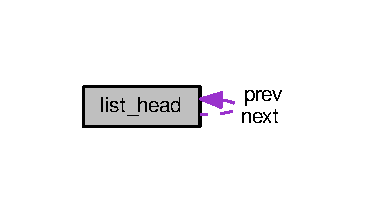
\includegraphics[width=176pt]{structlist__head__coll__graph}
\end{center}
\end{figure}
\subsection*{Atributos públicos}
\begin{DoxyCompactItemize}
\item 
struct \hyperlink{structlist__head}{list\+\_\+head} $\ast$ \hyperlink{structlist__head_ac3b0ff0dfb978a0cfbdad6b9d19cdcfe}{next}
\item 
struct \hyperlink{structlist__head}{list\+\_\+head} $\ast$ \hyperlink{structlist__head_aaa0eabda8877e1d6de73a33f223ad004}{prev}
\end{DoxyCompactItemize}


\subsection{Descripción detallada}


Definición en la línea 20 del archivo G-\/2313-\/06-\/\+P1\+\_\+list.\+h.



\subsection{Documentación de los datos miembro}
\hypertarget{structlist__head_ac3b0ff0dfb978a0cfbdad6b9d19cdcfe}{}\index{list\+\_\+head@{list\+\_\+head}!next@{next}}
\index{next@{next}!list\+\_\+head@{list\+\_\+head}}
\subsubsection[{next}]{\setlength{\rightskip}{0pt plus 5cm}struct {\bf list\+\_\+head}$\ast$ list\+\_\+head\+::next}\label{structlist__head_ac3b0ff0dfb978a0cfbdad6b9d19cdcfe}


Definición en la línea 21 del archivo G-\/2313-\/06-\/\+P1\+\_\+list.\+h.

\hypertarget{structlist__head_aaa0eabda8877e1d6de73a33f223ad004}{}\index{list\+\_\+head@{list\+\_\+head}!prev@{prev}}
\index{prev@{prev}!list\+\_\+head@{list\+\_\+head}}
\subsubsection[{prev}]{\setlength{\rightskip}{0pt plus 5cm}struct {\bf list\+\_\+head} $\ast$ list\+\_\+head\+::prev}\label{structlist__head_aaa0eabda8877e1d6de73a33f223ad004}


Definición en la línea 21 del archivo G-\/2313-\/06-\/\+P1\+\_\+list.\+h.



La documentación para esta estructura fue generada a partir del siguiente fichero\+:\begin{DoxyCompactItemize}
\item 
includes/\hyperlink{G-2313-06-P1__list_8h}{G-\/2313-\/06-\/\+P1\+\_\+list.\+h}\end{DoxyCompactItemize}

\hypertarget{structtask__t}{}\section{Referencia de la Estructura task\+\_\+t}
\label{structtask__t}\index{task\+\_\+t@{task\+\_\+t}}


{\ttfamily \#include $<$G-\/2313-\/06-\/\+P1\+\_\+thread\+\_\+pool.\+h$>$}



Diagrama de colaboración para task\+\_\+t\+:\nopagebreak
\begin{figure}[H]
\begin{center}
\leavevmode
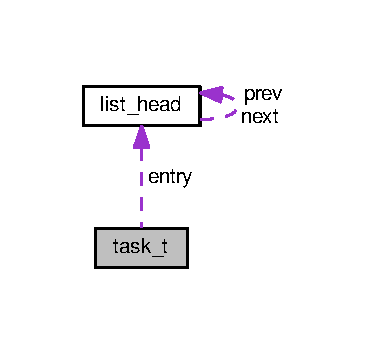
\includegraphics[width=176pt]{structtask__t__coll__graph}
\end{center}
\end{figure}
\subsection*{Atributos públicos}
\begin{DoxyCompactItemize}
\item 
int \hyperlink{structtask__t_a9162b404bd1cf5349b2092f69e31c613}{arg}
\item 
void $\ast$($\ast$ \hyperlink{structtask__t_ac8c2d416888e415fc6ee54410a4c511c}{task\+\_\+callback} )(int \hyperlink{structtask__t_a9162b404bd1cf5349b2092f69e31c613}{arg})
\item 
struct \hyperlink{structlist__head}{list\+\_\+head} \hyperlink{structtask__t_ac812553758f9102a7a674ad29e78f98b}{entry}
\end{DoxyCompactItemize}


\subsection{Descripción detallada}


Definición en la línea 28 del archivo G-\/2313-\/06-\/\+P1\+\_\+thread\+\_\+pool.\+h.



\subsection{Documentación de los datos miembro}
\hypertarget{structtask__t_a9162b404bd1cf5349b2092f69e31c613}{}\index{task\+\_\+t@{task\+\_\+t}!arg@{arg}}
\index{arg@{arg}!task\+\_\+t@{task\+\_\+t}}
\subsubsection[{arg}]{\setlength{\rightskip}{0pt plus 5cm}int task\+\_\+t\+::arg}\label{structtask__t_a9162b404bd1cf5349b2092f69e31c613}


Definición en la línea 30 del archivo G-\/2313-\/06-\/\+P1\+\_\+thread\+\_\+pool.\+h.

\hypertarget{structtask__t_ac812553758f9102a7a674ad29e78f98b}{}\index{task\+\_\+t@{task\+\_\+t}!entry@{entry}}
\index{entry@{entry}!task\+\_\+t@{task\+\_\+t}}
\subsubsection[{entry}]{\setlength{\rightskip}{0pt plus 5cm}struct {\bf list\+\_\+head} task\+\_\+t\+::entry}\label{structtask__t_ac812553758f9102a7a674ad29e78f98b}


Definición en la línea 32 del archivo G-\/2313-\/06-\/\+P1\+\_\+thread\+\_\+pool.\+h.

\hypertarget{structtask__t_ac8c2d416888e415fc6ee54410a4c511c}{}\index{task\+\_\+t@{task\+\_\+t}!task\+\_\+callback@{task\+\_\+callback}}
\index{task\+\_\+callback@{task\+\_\+callback}!task\+\_\+t@{task\+\_\+t}}
\subsubsection[{task\+\_\+callback}]{\setlength{\rightskip}{0pt plus 5cm}void$\ast$($\ast$ task\+\_\+t\+::task\+\_\+callback) (int {\bf arg})}\label{structtask__t_ac8c2d416888e415fc6ee54410a4c511c}


Definición en la línea 31 del archivo G-\/2313-\/06-\/\+P1\+\_\+thread\+\_\+pool.\+h.



La documentación para esta estructura fue generada a partir del siguiente fichero\+:\begin{DoxyCompactItemize}
\item 
includes/\hyperlink{G-2313-06-P1__thread__pool_8h}{G-\/2313-\/06-\/\+P1\+\_\+thread\+\_\+pool.\+h}\end{DoxyCompactItemize}

\hypertarget{structthread__args}{}\section{Referencia de la Estructura thread\+\_\+args}
\label{structthread__args}\index{thread\+\_\+args@{thread\+\_\+args}}


{\ttfamily \#include $<$G-\/2313-\/06-\/\+P1\+\_\+thread\+\_\+pool.\+h$>$}



Diagrama de colaboración para thread\+\_\+args\+:\nopagebreak
\begin{figure}[H]
\begin{center}
\leavevmode
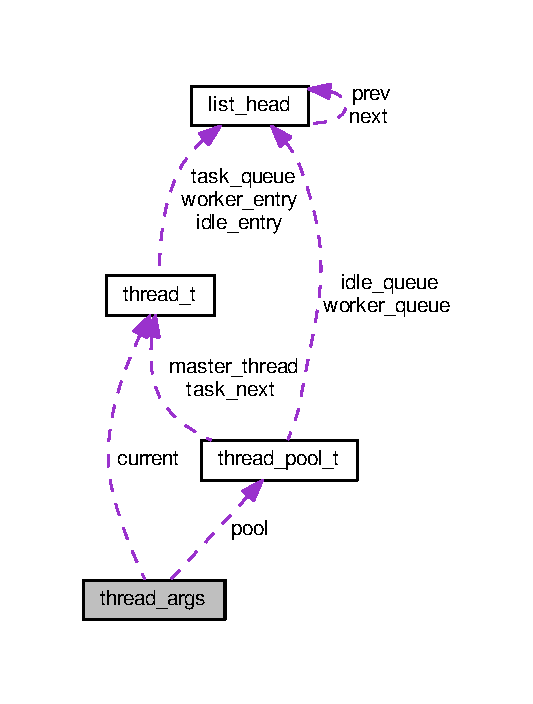
\includegraphics[width=256pt]{structthread__args__coll__graph}
\end{center}
\end{figure}
\subsection*{Atributos públicos}
\begin{DoxyCompactItemize}
\item 
struct \hyperlink{structthread__pool__t}{thread\+\_\+pool\+\_\+t} $\ast$ \hyperlink{structthread__args_a425ced5f77dcbb52f61d240a4e207a27}{pool}
\item 
struct \hyperlink{structthread__t}{thread\+\_\+t} $\ast$ \hyperlink{structthread__args_a191f3ea514283452d04bde31cde4c7ad}{current}
\end{DoxyCompactItemize}


\subsection{Descripción detallada}


Definición en la línea 63 del archivo G-\/2313-\/06-\/\+P1\+\_\+thread\+\_\+pool.\+h.



\subsection{Documentación de los datos miembro}
\hypertarget{structthread__args_a191f3ea514283452d04bde31cde4c7ad}{}\index{thread\+\_\+args@{thread\+\_\+args}!current@{current}}
\index{current@{current}!thread\+\_\+args@{thread\+\_\+args}}
\subsubsection[{current}]{\setlength{\rightskip}{0pt plus 5cm}struct {\bf thread\+\_\+t}$\ast$ thread\+\_\+args\+::current}\label{structthread__args_a191f3ea514283452d04bde31cde4c7ad}


Definición en la línea 65 del archivo G-\/2313-\/06-\/\+P1\+\_\+thread\+\_\+pool.\+h.

\hypertarget{structthread__args_a425ced5f77dcbb52f61d240a4e207a27}{}\index{thread\+\_\+args@{thread\+\_\+args}!pool@{pool}}
\index{pool@{pool}!thread\+\_\+args@{thread\+\_\+args}}
\subsubsection[{pool}]{\setlength{\rightskip}{0pt plus 5cm}struct {\bf thread\+\_\+pool\+\_\+t}$\ast$ thread\+\_\+args\+::pool}\label{structthread__args_a425ced5f77dcbb52f61d240a4e207a27}


Definición en la línea 64 del archivo G-\/2313-\/06-\/\+P1\+\_\+thread\+\_\+pool.\+h.



La documentación para esta estructura fue generada a partir del siguiente fichero\+:\begin{DoxyCompactItemize}
\item 
includes/\hyperlink{G-2313-06-P1__thread__pool_8h}{G-\/2313-\/06-\/\+P1\+\_\+thread\+\_\+pool.\+h}\end{DoxyCompactItemize}

\hypertarget{structthread__pool__t}{}\section{Referencia de la Estructura thread\+\_\+pool\+\_\+t}
\label{structthread__pool__t}\index{thread\+\_\+pool\+\_\+t@{thread\+\_\+pool\+\_\+t}}


{\ttfamily \#include $<$G-\/2313-\/06-\/\+P1\+\_\+thread\+\_\+pool.\+h$>$}



Diagrama de colaboración para thread\+\_\+pool\+\_\+t\+:\nopagebreak
\begin{figure}[H]
\begin{center}
\leavevmode
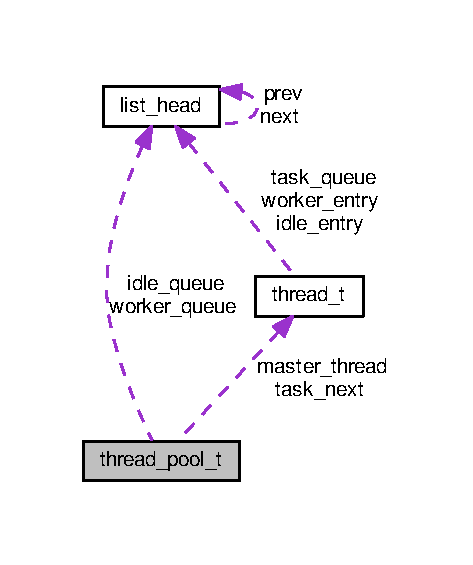
\includegraphics[width=227pt]{structthread__pool__t__coll__graph}
\end{center}
\end{figure}
\subsection*{Atributos públicos}
\begin{DoxyCompactItemize}
\item 
struct \hyperlink{structlist__head}{list\+\_\+head} \hyperlink{structthread__pool__t_a44640e57780a54d437d7589b1c754ac1}{worker\+\_\+queue}
\item 
struct \hyperlink{structlist__head}{list\+\_\+head} \hyperlink{structthread__pool__t_a38a9fa0d0ea1060d5bbff8421a92c1c7}{idle\+\_\+queue}
\item 
\hyperlink{structthread__t}{thread\+\_\+t} $\ast$ \hyperlink{structthread__pool__t_a9ad8218717dde39eef701a8bce5ca0a1}{master\+\_\+thread}
\item 
pthread\+\_\+mutex\+\_\+t \hyperlink{structthread__pool__t_aaa6e0a9d9c28c3f9be7eccbe8003af23}{global}
\item 
\hyperlink{structthread__t}{thread\+\_\+t} $\ast$ \hyperlink{structthread__pool__t_a00ce5a27204f85e624552f7448ba7093}{task\+\_\+next}
\item 
int \hyperlink{structthread__pool__t_a3185c157636a142415699a20042d6dd8}{size}
\item 
int \hyperlink{structthread__pool__t_a978e7f94032dad6e7a373e7bc1896237}{max\+\_\+size}
\item 
int \hyperlink{structthread__pool__t_a80aa1805a11e2e6e2bf5811fda0ffc26}{min\+\_\+size}
\item 
double \hyperlink{structthread__pool__t_a815792ab9c936b06d46ef3e149e5fd88}{low\+\_\+level}
\item 
double \hyperlink{structthread__pool__t_aa771fc181f63c16346fff1c7eb0d9014}{high\+\_\+level}
\item 
int \hyperlink{structthread__pool__t_ae3eaf8d90ef550166e595286a6175d14}{master\+\_\+interval}
\end{DoxyCompactItemize}


\subsection{Descripción detallada}


Definición en la línea 48 del archivo G-\/2313-\/06-\/\+P1\+\_\+thread\+\_\+pool.\+h.



\subsection{Documentación de los datos miembro}
\hypertarget{structthread__pool__t_aaa6e0a9d9c28c3f9be7eccbe8003af23}{}\index{thread\+\_\+pool\+\_\+t@{thread\+\_\+pool\+\_\+t}!global@{global}}
\index{global@{global}!thread\+\_\+pool\+\_\+t@{thread\+\_\+pool\+\_\+t}}
\subsubsection[{global}]{\setlength{\rightskip}{0pt plus 5cm}pthread\+\_\+mutex\+\_\+t thread\+\_\+pool\+\_\+t\+::global}\label{structthread__pool__t_aaa6e0a9d9c28c3f9be7eccbe8003af23}


Definición en la línea 53 del archivo G-\/2313-\/06-\/\+P1\+\_\+thread\+\_\+pool.\+h.

\hypertarget{structthread__pool__t_aa771fc181f63c16346fff1c7eb0d9014}{}\index{thread\+\_\+pool\+\_\+t@{thread\+\_\+pool\+\_\+t}!high\+\_\+level@{high\+\_\+level}}
\index{high\+\_\+level@{high\+\_\+level}!thread\+\_\+pool\+\_\+t@{thread\+\_\+pool\+\_\+t}}
\subsubsection[{high\+\_\+level}]{\setlength{\rightskip}{0pt plus 5cm}double thread\+\_\+pool\+\_\+t\+::high\+\_\+level}\label{structthread__pool__t_aa771fc181f63c16346fff1c7eb0d9014}


Definición en la línea 59 del archivo G-\/2313-\/06-\/\+P1\+\_\+thread\+\_\+pool.\+h.

\hypertarget{structthread__pool__t_a38a9fa0d0ea1060d5bbff8421a92c1c7}{}\index{thread\+\_\+pool\+\_\+t@{thread\+\_\+pool\+\_\+t}!idle\+\_\+queue@{idle\+\_\+queue}}
\index{idle\+\_\+queue@{idle\+\_\+queue}!thread\+\_\+pool\+\_\+t@{thread\+\_\+pool\+\_\+t}}
\subsubsection[{idle\+\_\+queue}]{\setlength{\rightskip}{0pt plus 5cm}struct {\bf list\+\_\+head} thread\+\_\+pool\+\_\+t\+::idle\+\_\+queue}\label{structthread__pool__t_a38a9fa0d0ea1060d5bbff8421a92c1c7}


Definición en la línea 51 del archivo G-\/2313-\/06-\/\+P1\+\_\+thread\+\_\+pool.\+h.

\hypertarget{structthread__pool__t_a815792ab9c936b06d46ef3e149e5fd88}{}\index{thread\+\_\+pool\+\_\+t@{thread\+\_\+pool\+\_\+t}!low\+\_\+level@{low\+\_\+level}}
\index{low\+\_\+level@{low\+\_\+level}!thread\+\_\+pool\+\_\+t@{thread\+\_\+pool\+\_\+t}}
\subsubsection[{low\+\_\+level}]{\setlength{\rightskip}{0pt plus 5cm}double thread\+\_\+pool\+\_\+t\+::low\+\_\+level}\label{structthread__pool__t_a815792ab9c936b06d46ef3e149e5fd88}


Definición en la línea 58 del archivo G-\/2313-\/06-\/\+P1\+\_\+thread\+\_\+pool.\+h.

\hypertarget{structthread__pool__t_ae3eaf8d90ef550166e595286a6175d14}{}\index{thread\+\_\+pool\+\_\+t@{thread\+\_\+pool\+\_\+t}!master\+\_\+interval@{master\+\_\+interval}}
\index{master\+\_\+interval@{master\+\_\+interval}!thread\+\_\+pool\+\_\+t@{thread\+\_\+pool\+\_\+t}}
\subsubsection[{master\+\_\+interval}]{\setlength{\rightskip}{0pt plus 5cm}int thread\+\_\+pool\+\_\+t\+::master\+\_\+interval}\label{structthread__pool__t_ae3eaf8d90ef550166e595286a6175d14}


Definición en la línea 60 del archivo G-\/2313-\/06-\/\+P1\+\_\+thread\+\_\+pool.\+h.

\hypertarget{structthread__pool__t_a9ad8218717dde39eef701a8bce5ca0a1}{}\index{thread\+\_\+pool\+\_\+t@{thread\+\_\+pool\+\_\+t}!master\+\_\+thread@{master\+\_\+thread}}
\index{master\+\_\+thread@{master\+\_\+thread}!thread\+\_\+pool\+\_\+t@{thread\+\_\+pool\+\_\+t}}
\subsubsection[{master\+\_\+thread}]{\setlength{\rightskip}{0pt plus 5cm}{\bf thread\+\_\+t}$\ast$ thread\+\_\+pool\+\_\+t\+::master\+\_\+thread}\label{structthread__pool__t_a9ad8218717dde39eef701a8bce5ca0a1}


Definición en la línea 52 del archivo G-\/2313-\/06-\/\+P1\+\_\+thread\+\_\+pool.\+h.

\hypertarget{structthread__pool__t_a978e7f94032dad6e7a373e7bc1896237}{}\index{thread\+\_\+pool\+\_\+t@{thread\+\_\+pool\+\_\+t}!max\+\_\+size@{max\+\_\+size}}
\index{max\+\_\+size@{max\+\_\+size}!thread\+\_\+pool\+\_\+t@{thread\+\_\+pool\+\_\+t}}
\subsubsection[{max\+\_\+size}]{\setlength{\rightskip}{0pt plus 5cm}int thread\+\_\+pool\+\_\+t\+::max\+\_\+size}\label{structthread__pool__t_a978e7f94032dad6e7a373e7bc1896237}


Definición en la línea 56 del archivo G-\/2313-\/06-\/\+P1\+\_\+thread\+\_\+pool.\+h.

\hypertarget{structthread__pool__t_a80aa1805a11e2e6e2bf5811fda0ffc26}{}\index{thread\+\_\+pool\+\_\+t@{thread\+\_\+pool\+\_\+t}!min\+\_\+size@{min\+\_\+size}}
\index{min\+\_\+size@{min\+\_\+size}!thread\+\_\+pool\+\_\+t@{thread\+\_\+pool\+\_\+t}}
\subsubsection[{min\+\_\+size}]{\setlength{\rightskip}{0pt plus 5cm}int thread\+\_\+pool\+\_\+t\+::min\+\_\+size}\label{structthread__pool__t_a80aa1805a11e2e6e2bf5811fda0ffc26}


Definición en la línea 57 del archivo G-\/2313-\/06-\/\+P1\+\_\+thread\+\_\+pool.\+h.

\hypertarget{structthread__pool__t_a3185c157636a142415699a20042d6dd8}{}\index{thread\+\_\+pool\+\_\+t@{thread\+\_\+pool\+\_\+t}!size@{size}}
\index{size@{size}!thread\+\_\+pool\+\_\+t@{thread\+\_\+pool\+\_\+t}}
\subsubsection[{size}]{\setlength{\rightskip}{0pt plus 5cm}int thread\+\_\+pool\+\_\+t\+::size}\label{structthread__pool__t_a3185c157636a142415699a20042d6dd8}


Definición en la línea 55 del archivo G-\/2313-\/06-\/\+P1\+\_\+thread\+\_\+pool.\+h.

\hypertarget{structthread__pool__t_a00ce5a27204f85e624552f7448ba7093}{}\index{thread\+\_\+pool\+\_\+t@{thread\+\_\+pool\+\_\+t}!task\+\_\+next@{task\+\_\+next}}
\index{task\+\_\+next@{task\+\_\+next}!thread\+\_\+pool\+\_\+t@{thread\+\_\+pool\+\_\+t}}
\subsubsection[{task\+\_\+next}]{\setlength{\rightskip}{0pt plus 5cm}{\bf thread\+\_\+t}$\ast$ thread\+\_\+pool\+\_\+t\+::task\+\_\+next}\label{structthread__pool__t_a00ce5a27204f85e624552f7448ba7093}


Definición en la línea 54 del archivo G-\/2313-\/06-\/\+P1\+\_\+thread\+\_\+pool.\+h.

\hypertarget{structthread__pool__t_a44640e57780a54d437d7589b1c754ac1}{}\index{thread\+\_\+pool\+\_\+t@{thread\+\_\+pool\+\_\+t}!worker\+\_\+queue@{worker\+\_\+queue}}
\index{worker\+\_\+queue@{worker\+\_\+queue}!thread\+\_\+pool\+\_\+t@{thread\+\_\+pool\+\_\+t}}
\subsubsection[{worker\+\_\+queue}]{\setlength{\rightskip}{0pt plus 5cm}struct {\bf list\+\_\+head} thread\+\_\+pool\+\_\+t\+::worker\+\_\+queue}\label{structthread__pool__t_a44640e57780a54d437d7589b1c754ac1}


Definición en la línea 50 del archivo G-\/2313-\/06-\/\+P1\+\_\+thread\+\_\+pool.\+h.



La documentación para esta estructura fue generada a partir del siguiente fichero\+:\begin{DoxyCompactItemize}
\item 
includes/\hyperlink{G-2313-06-P1__thread__pool_8h}{G-\/2313-\/06-\/\+P1\+\_\+thread\+\_\+pool.\+h}\end{DoxyCompactItemize}

\hypertarget{structthread__t}{}\section{Referencia de la Estructura thread\+\_\+t}
\label{structthread__t}\index{thread\+\_\+t@{thread\+\_\+t}}


{\ttfamily \#include $<$G-\/2313-\/06-\/\+P1\+\_\+thread\+\_\+pool.\+h$>$}



Diagrama de colaboración para thread\+\_\+t\+:
% FIG 0
\subsection*{Atributos públicos}
\begin{DoxyCompactItemize}
\item 
pthread\+\_\+t \hyperlink{structthread__t_a92c076d58ca307499452b8dfe0c4e598}{tid}
\item 
pthread\+\_\+mutex\+\_\+t \hyperlink{structthread__t_abb0dcb82ff12b61776b74c76fa27c964}{mutex}
\item 
pthread\+\_\+cond\+\_\+t \hyperlink{structthread__t_a6cb846b84c59d01a8b3a2693d39a4af1}{cond}
\item 
int \hyperlink{structthread__t_a3e0780f1c2fc9932258a60b5043fe424}{state}
\item 
int \hyperlink{structthread__t_a8e9f0fd028676d0ebeef8438f2176bb7}{stop}
\item 
int \hyperlink{structthread__t_aa99eeab6834595bdff5a7da08314fd89}{queue\+\_\+size}
\item 
struct \hyperlink{structlist__head}{list\+\_\+head} \hyperlink{structthread__t_a69c932ede0de60b66a482fb735fca966}{task\+\_\+queue}
\item 
struct \hyperlink{structlist__head}{list\+\_\+head} \hyperlink{structthread__t_a03432229de426c5ba35d0dfa325491f0}{worker\+\_\+entry}
\item 
struct \hyperlink{structlist__head}{list\+\_\+head} \hyperlink{structthread__t_a9386032d478cacdfd680d5691e0eb9d3}{idle\+\_\+entry}
\end{DoxyCompactItemize}


\subsection{Descripción detallada}


Definición en la línea 35 del archivo G-\/2313-\/06-\/\+P1\+\_\+thread\+\_\+pool.\+h.



\subsection{Documentación de los datos miembro}
\index{thread\+\_\+t@{thread\+\_\+t}!cond@{cond}}
\index{cond@{cond}!thread\+\_\+t@{thread\+\_\+t}}
\subsubsection[{\texorpdfstring{cond}{cond}}]{\setlength{\rightskip}{0pt plus 5cm}pthread\+\_\+cond\+\_\+t thread\+\_\+t\+::cond}\hypertarget{structthread__t_a6cb846b84c59d01a8b3a2693d39a4af1}{}\label{structthread__t_a6cb846b84c59d01a8b3a2693d39a4af1}


Definición en la línea 39 del archivo G-\/2313-\/06-\/\+P1\+\_\+thread\+\_\+pool.\+h.

\index{thread\+\_\+t@{thread\+\_\+t}!idle\+\_\+entry@{idle\+\_\+entry}}
\index{idle\+\_\+entry@{idle\+\_\+entry}!thread\+\_\+t@{thread\+\_\+t}}
\subsubsection[{\texorpdfstring{idle\+\_\+entry}{idle_entry}}]{\setlength{\rightskip}{0pt plus 5cm}struct {\bf list\+\_\+head} thread\+\_\+t\+::idle\+\_\+entry}\hypertarget{structthread__t_a9386032d478cacdfd680d5691e0eb9d3}{}\label{structthread__t_a9386032d478cacdfd680d5691e0eb9d3}


Definición en la línea 45 del archivo G-\/2313-\/06-\/\+P1\+\_\+thread\+\_\+pool.\+h.

\index{thread\+\_\+t@{thread\+\_\+t}!mutex@{mutex}}
\index{mutex@{mutex}!thread\+\_\+t@{thread\+\_\+t}}
\subsubsection[{\texorpdfstring{mutex}{mutex}}]{\setlength{\rightskip}{0pt plus 5cm}pthread\+\_\+mutex\+\_\+t thread\+\_\+t\+::mutex}\hypertarget{structthread__t_abb0dcb82ff12b61776b74c76fa27c964}{}\label{structthread__t_abb0dcb82ff12b61776b74c76fa27c964}


Definición en la línea 38 del archivo G-\/2313-\/06-\/\+P1\+\_\+thread\+\_\+pool.\+h.

\index{thread\+\_\+t@{thread\+\_\+t}!queue\+\_\+size@{queue\+\_\+size}}
\index{queue\+\_\+size@{queue\+\_\+size}!thread\+\_\+t@{thread\+\_\+t}}
\subsubsection[{\texorpdfstring{queue\+\_\+size}{queue_size}}]{\setlength{\rightskip}{0pt plus 5cm}int thread\+\_\+t\+::queue\+\_\+size}\hypertarget{structthread__t_aa99eeab6834595bdff5a7da08314fd89}{}\label{structthread__t_aa99eeab6834595bdff5a7da08314fd89}


Definición en la línea 42 del archivo G-\/2313-\/06-\/\+P1\+\_\+thread\+\_\+pool.\+h.

\index{thread\+\_\+t@{thread\+\_\+t}!state@{state}}
\index{state@{state}!thread\+\_\+t@{thread\+\_\+t}}
\subsubsection[{\texorpdfstring{state}{state}}]{\setlength{\rightskip}{0pt plus 5cm}int thread\+\_\+t\+::state}\hypertarget{structthread__t_a3e0780f1c2fc9932258a60b5043fe424}{}\label{structthread__t_a3e0780f1c2fc9932258a60b5043fe424}


Definición en la línea 40 del archivo G-\/2313-\/06-\/\+P1\+\_\+thread\+\_\+pool.\+h.

\index{thread\+\_\+t@{thread\+\_\+t}!stop@{stop}}
\index{stop@{stop}!thread\+\_\+t@{thread\+\_\+t}}
\subsubsection[{\texorpdfstring{stop}{stop}}]{\setlength{\rightskip}{0pt plus 5cm}int thread\+\_\+t\+::stop}\hypertarget{structthread__t_a8e9f0fd028676d0ebeef8438f2176bb7}{}\label{structthread__t_a8e9f0fd028676d0ebeef8438f2176bb7}


Definición en la línea 41 del archivo G-\/2313-\/06-\/\+P1\+\_\+thread\+\_\+pool.\+h.

\index{thread\+\_\+t@{thread\+\_\+t}!task\+\_\+queue@{task\+\_\+queue}}
\index{task\+\_\+queue@{task\+\_\+queue}!thread\+\_\+t@{thread\+\_\+t}}
\subsubsection[{\texorpdfstring{task\+\_\+queue}{task_queue}}]{\setlength{\rightskip}{0pt plus 5cm}struct {\bf list\+\_\+head} thread\+\_\+t\+::task\+\_\+queue}\hypertarget{structthread__t_a69c932ede0de60b66a482fb735fca966}{}\label{structthread__t_a69c932ede0de60b66a482fb735fca966}


Definición en la línea 43 del archivo G-\/2313-\/06-\/\+P1\+\_\+thread\+\_\+pool.\+h.

\index{thread\+\_\+t@{thread\+\_\+t}!tid@{tid}}
\index{tid@{tid}!thread\+\_\+t@{thread\+\_\+t}}
\subsubsection[{\texorpdfstring{tid}{tid}}]{\setlength{\rightskip}{0pt plus 5cm}pthread\+\_\+t thread\+\_\+t\+::tid}\hypertarget{structthread__t_a92c076d58ca307499452b8dfe0c4e598}{}\label{structthread__t_a92c076d58ca307499452b8dfe0c4e598}


Definición en la línea 37 del archivo G-\/2313-\/06-\/\+P1\+\_\+thread\+\_\+pool.\+h.

\index{thread\+\_\+t@{thread\+\_\+t}!worker\+\_\+entry@{worker\+\_\+entry}}
\index{worker\+\_\+entry@{worker\+\_\+entry}!thread\+\_\+t@{thread\+\_\+t}}
\subsubsection[{\texorpdfstring{worker\+\_\+entry}{worker_entry}}]{\setlength{\rightskip}{0pt plus 5cm}struct {\bf list\+\_\+head} thread\+\_\+t\+::worker\+\_\+entry}\hypertarget{structthread__t_a03432229de426c5ba35d0dfa325491f0}{}\label{structthread__t_a03432229de426c5ba35d0dfa325491f0}


Definición en la línea 44 del archivo G-\/2313-\/06-\/\+P1\+\_\+thread\+\_\+pool.\+h.



La documentación para esta estructura fue generada a partir del siguiente fichero\+:\begin{DoxyCompactItemize}
\item 
includes/\hyperlink{G-2313-06-P1__thread__pool_8h}{G-\/2313-\/06-\/\+P1\+\_\+thread\+\_\+pool.\+h}\end{DoxyCompactItemize}

\chapter{Documentación de archivos}
\hypertarget{G-2313-06-P1__common__functions_8h}{}\section{Referencia del Archivo includes/\+G-\/2313-\/06-\/\+P1\+\_\+common\+\_\+functions.h}
\label{G-2313-06-P1__common__functions_8h}\index{includes/\+G-\/2313-\/06-\/\+P1\+\_\+common\+\_\+functions.\+h@{includes/\+G-\/2313-\/06-\/\+P1\+\_\+common\+\_\+functions.\+h}}
{\ttfamily \#include $<$unistd.\+h$>$}\\*
{\ttfamily \#include $<$sys/types.\+h$>$}\\*
{\ttfamily \#include $<$sys/socket.\+h$>$}\\*
{\ttfamily \#include $<$sys/stat.\+h$>$}\\*
{\ttfamily \#include $<$netinet/in.\+h$>$}\\*
{\ttfamily \#include $<$syslog.\+h$>$}\\*
{\ttfamily \#include $<$stdlib.\+h$>$}\\*
{\ttfamily \#include $<$stdio.\+h$>$}\\*
{\ttfamily \#include $<$strings.\+h$>$}\\*
{\ttfamily \#include $<$signal.\+h$>$}\\*
{\ttfamily \#include $<$stdbool.\+h$>$}\\*
{\ttfamily \#include $<$time.\+h$>$}\\*
{\ttfamily \#include $<$arpa/inet.\+h$>$}\\*
{\ttfamily \#include $<$redes2/irc.\+h$>$}\\*
{\ttfamily \#include $<$netdb.\+h$>$}\\*
{\ttfamily \#include $<$pthread.\+h$>$}\\*
Dependencia gráfica adjunta para G-\/2313-\/06-\/\+P1\+\_\+common\+\_\+functions.h\+:

\hypertarget{G-2313-06-P1__function__handlers_8h}{}\section{Referencia del Archivo includes/\+G-\/2313-\/06-\/\+P1\+\_\+function\+\_\+handlers.h}
\label{G-2313-06-P1__function__handlers_8h}\index{includes/\+G-\/2313-\/06-\/\+P1\+\_\+function\+\_\+handlers.\+h@{includes/\+G-\/2313-\/06-\/\+P1\+\_\+function\+\_\+handlers.\+h}}
{\ttfamily \#include $<$unistd.\+h$>$}\\*
{\ttfamily \#include $<$sys/types.\+h$>$}\\*
{\ttfamily \#include $<$sys/socket.\+h$>$}\\*
{\ttfamily \#include $<$sys/stat.\+h$>$}\\*
{\ttfamily \#include $<$netinet/in.\+h$>$}\\*
{\ttfamily \#include $<$syslog.\+h$>$}\\*
{\ttfamily \#include $<$stdlib.\+h$>$}\\*
{\ttfamily \#include $<$stdio.\+h$>$}\\*
{\ttfamily \#include $<$strings.\+h$>$}\\*
{\ttfamily \#include $<$signal.\+h$>$}\\*
{\ttfamily \#include $<$stdbool.\+h$>$}\\*
{\ttfamily \#include $<$time.\+h$>$}\\*
{\ttfamily \#include $<$arpa/inet.\+h$>$}\\*
{\ttfamily \#include $<$redes2/irc.\+h$>$}\\*
{\ttfamily \#include $<$netdb.\+h$>$}\\*
{\ttfamily \#include $<$pthread.\+h$>$}\\*
{\ttfamily \#include \char`\"{}G-\/2313-\/06-\/\+P1\+\_\+common\+\_\+functions.\+h\char`\"{}}\\*
Dependencia gráfica adjunta para G-\/2313-\/06-\/\+P1\+\_\+function\+\_\+handlers.h\+:
% FIG 0
Gráfico de los archivos que directa o indirectamente incluyen a este archivo\+:
% FIG 1
\subsection*{Funciones}
\begin{DoxyCompactItemize}
\item 
void \hyperlink{G-2313-06-P1__function__handlers_8h_aeefab469ba48ce1655dd5afd14f104b4}{server\+\_\+command\+\_\+nick} (char $\ast$command, int desc, char $\ast$nick\+\_\+static, int $\ast$register\+\_\+status)
\item 
void \hyperlink{G-2313-06-P1__function__handlers_8h_ad09156d6bd4cf58f4345e0bf851ff099}{server\+\_\+command\+\_\+user} (char $\ast$command, int desc, char $\ast$nick\+\_\+static, int $\ast$register\+\_\+status)
\item 
void \hyperlink{G-2313-06-P1__function__handlers_8h_a375c143c5469d1bb4fa7793b310ad68e}{server\+\_\+command\+\_\+join} (char $\ast$command, int desc, char $\ast$nick\+\_\+static, int $\ast$register\+\_\+status)
\item 
void \hyperlink{G-2313-06-P1__function__handlers_8h_a3df99a1f2cefc2d91d65cbb6dd555f96}{server\+\_\+command\+\_\+quit} (char $\ast$command, int desc, char $\ast$nick\+\_\+static, int $\ast$register\+\_\+status)
\item 
void \hyperlink{G-2313-06-P1__function__handlers_8h_acc1c181bf44087b9216d1b59809937aa}{server\+\_\+command\+\_\+ping} (char $\ast$command, int desc, char $\ast$nick\+\_\+static, int $\ast$register\+\_\+status)
\item 
void \hyperlink{G-2313-06-P1__function__handlers_8h_af289e3cc397e24e9b8c12c35bce68285}{server\+\_\+command\+\_\+list} (char $\ast$command, int desc, char $\ast$nick\+\_\+static, int $\ast$register\+\_\+status)
\item 
void \hyperlink{G-2313-06-P1__function__handlers_8h_a8daf68135f2d9e9412c04a2980bdfb2f}{server\+\_\+command\+\_\+privmsg} (char $\ast$command, int desc, char $\ast$nick\+\_\+static, int $\ast$register\+\_\+status)
\item 
void \hyperlink{G-2313-06-P1__function__handlers_8h_aba1a3da1fb58bb35076e7ea56037463e}{server\+\_\+command\+\_\+part} (char $\ast$command, int desc, char $\ast$nick\+\_\+static, int $\ast$register\+\_\+status)
\item 
void \hyperlink{G-2313-06-P1__function__handlers_8h_a0fe05d80af27ae220f8fa631468606ea}{server\+\_\+command\+\_\+names} (char $\ast$command, int desc, char $\ast$nick\+\_\+static, int $\ast$register\+\_\+status)
\item 
void \hyperlink{G-2313-06-P1__function__handlers_8h_a33025bd9c7bf8fbb2bf9cf722c07465c}{server\+\_\+command\+\_\+kick} (char $\ast$command, int desc, char $\ast$nick\+\_\+static, int $\ast$register\+\_\+status)
\item 
void \hyperlink{G-2313-06-P1__function__handlers_8h_a44a8736512c1df49d94c8194ae9b8a50}{server\+\_\+command\+\_\+mode} (char $\ast$command, int desc, char $\ast$nick\+\_\+static, int $\ast$register\+\_\+status)
\item 
void \hyperlink{G-2313-06-P1__function__handlers_8h_a327516a6c48e34b58428f7a502938928}{server\+\_\+command\+\_\+away} (char $\ast$command, int desc, char $\ast$nick\+\_\+static, int $\ast$register\+\_\+status)
\item 
void \hyperlink{G-2313-06-P1__function__handlers_8h_a8bb934f01707fcb12ebac41f1fe69441}{server\+\_\+command\+\_\+whois} (char $\ast$command, int desc, char $\ast$nick\+\_\+static, int $\ast$register\+\_\+status)
\item 
void \hyperlink{G-2313-06-P1__function__handlers_8h_a894ae019e03841e9d54fdad31d79f218}{server\+\_\+command\+\_\+topic} (char $\ast$command, int desc, char $\ast$nick\+\_\+static, int $\ast$register\+\_\+status)
\item 
void \hyperlink{G-2313-06-P1__function__handlers_8h_a1258d3bdf779b82c3f952bdde3d62631}{server\+\_\+command\+\_\+motd} (char $\ast$command, int desc, char $\ast$nick\+\_\+static, int $\ast$register\+\_\+status)
\end{DoxyCompactItemize}


\subsection{Documentación de las funciones}
\index{G-\/2313-\/06-\/\+P1\+\_\+function\+\_\+handlers.\+h@{G-\/2313-\/06-\/\+P1\+\_\+function\+\_\+handlers.\+h}!server\+\_\+command\+\_\+away@{server\+\_\+command\+\_\+away}}
\index{server\+\_\+command\+\_\+away@{server\+\_\+command\+\_\+away}!G-\/2313-\/06-\/\+P1\+\_\+function\+\_\+handlers.\+h@{G-\/2313-\/06-\/\+P1\+\_\+function\+\_\+handlers.\+h}}
\subsubsection[{\texorpdfstring{server\+\_\+command\+\_\+away(char $\ast$command, int desc, char $\ast$nick\+\_\+static, int $\ast$register\+\_\+status)}{server_command_away(char *command, int desc, char *nick_static, int *register_status)}}]{\setlength{\rightskip}{0pt plus 5cm}void server\+\_\+command\+\_\+away (
\begin{DoxyParamCaption}
\item[{char $\ast$}]{command, }
\item[{int}]{desc, }
\item[{char $\ast$}]{nick\+\_\+static, }
\item[{int $\ast$}]{register\+\_\+status}
\end{DoxyParamCaption}
)}\hypertarget{G-2313-06-P1__function__handlers_8h_a327516a6c48e34b58428f7a502938928}{}\label{G-2313-06-P1__function__handlers_8h_a327516a6c48e34b58428f7a502938928}


Definición en la línea 1046 del archivo G-\/2313-\/06-\/\+P1\+\_\+function\+\_\+handlers.\+c.

\index{G-\/2313-\/06-\/\+P1\+\_\+function\+\_\+handlers.\+h@{G-\/2313-\/06-\/\+P1\+\_\+function\+\_\+handlers.\+h}!server\+\_\+command\+\_\+join@{server\+\_\+command\+\_\+join}}
\index{server\+\_\+command\+\_\+join@{server\+\_\+command\+\_\+join}!G-\/2313-\/06-\/\+P1\+\_\+function\+\_\+handlers.\+h@{G-\/2313-\/06-\/\+P1\+\_\+function\+\_\+handlers.\+h}}
\subsubsection[{\texorpdfstring{server\+\_\+command\+\_\+join(char $\ast$command, int desc, char $\ast$nick\+\_\+static, int $\ast$register\+\_\+status)}{server_command_join(char *command, int desc, char *nick_static, int *register_status)}}]{\setlength{\rightskip}{0pt plus 5cm}void server\+\_\+command\+\_\+join (
\begin{DoxyParamCaption}
\item[{char $\ast$}]{command, }
\item[{int}]{desc, }
\item[{char $\ast$}]{nick\+\_\+static, }
\item[{int $\ast$}]{register\+\_\+status}
\end{DoxyParamCaption}
)}\hypertarget{G-2313-06-P1__function__handlers_8h_a375c143c5469d1bb4fa7793b310ad68e}{}\label{G-2313-06-P1__function__handlers_8h_a375c143c5469d1bb4fa7793b310ad68e}


Definición en la línea 255 del archivo G-\/2313-\/06-\/\+P1\+\_\+function\+\_\+handlers.\+c.

\index{G-\/2313-\/06-\/\+P1\+\_\+function\+\_\+handlers.\+h@{G-\/2313-\/06-\/\+P1\+\_\+function\+\_\+handlers.\+h}!server\+\_\+command\+\_\+kick@{server\+\_\+command\+\_\+kick}}
\index{server\+\_\+command\+\_\+kick@{server\+\_\+command\+\_\+kick}!G-\/2313-\/06-\/\+P1\+\_\+function\+\_\+handlers.\+h@{G-\/2313-\/06-\/\+P1\+\_\+function\+\_\+handlers.\+h}}
\subsubsection[{\texorpdfstring{server\+\_\+command\+\_\+kick(char $\ast$command, int desc, char $\ast$nick\+\_\+static, int $\ast$register\+\_\+status)}{server_command_kick(char *command, int desc, char *nick_static, int *register_status)}}]{\setlength{\rightskip}{0pt plus 5cm}void server\+\_\+command\+\_\+kick (
\begin{DoxyParamCaption}
\item[{char $\ast$}]{command, }
\item[{int}]{desc, }
\item[{char $\ast$}]{nick\+\_\+static, }
\item[{int $\ast$}]{register\+\_\+status}
\end{DoxyParamCaption}
)}\hypertarget{G-2313-06-P1__function__handlers_8h_a33025bd9c7bf8fbb2bf9cf722c07465c}{}\label{G-2313-06-P1__function__handlers_8h_a33025bd9c7bf8fbb2bf9cf722c07465c}


Definición en la línea 808 del archivo G-\/2313-\/06-\/\+P1\+\_\+function\+\_\+handlers.\+c.

\index{G-\/2313-\/06-\/\+P1\+\_\+function\+\_\+handlers.\+h@{G-\/2313-\/06-\/\+P1\+\_\+function\+\_\+handlers.\+h}!server\+\_\+command\+\_\+list@{server\+\_\+command\+\_\+list}}
\index{server\+\_\+command\+\_\+list@{server\+\_\+command\+\_\+list}!G-\/2313-\/06-\/\+P1\+\_\+function\+\_\+handlers.\+h@{G-\/2313-\/06-\/\+P1\+\_\+function\+\_\+handlers.\+h}}
\subsubsection[{\texorpdfstring{server\+\_\+command\+\_\+list(char $\ast$command, int desc, char $\ast$nick\+\_\+static, int $\ast$register\+\_\+status)}{server_command_list(char *command, int desc, char *nick_static, int *register_status)}}]{\setlength{\rightskip}{0pt plus 5cm}void server\+\_\+command\+\_\+list (
\begin{DoxyParamCaption}
\item[{char $\ast$}]{command, }
\item[{int}]{desc, }
\item[{char $\ast$}]{nick\+\_\+static, }
\item[{int $\ast$}]{register\+\_\+status}
\end{DoxyParamCaption}
)}\hypertarget{G-2313-06-P1__function__handlers_8h_af289e3cc397e24e9b8c12c35bce68285}{}\label{G-2313-06-P1__function__handlers_8h_af289e3cc397e24e9b8c12c35bce68285}


Definición en la línea 472 del archivo G-\/2313-\/06-\/\+P1\+\_\+function\+\_\+handlers.\+c.

\index{G-\/2313-\/06-\/\+P1\+\_\+function\+\_\+handlers.\+h@{G-\/2313-\/06-\/\+P1\+\_\+function\+\_\+handlers.\+h}!server\+\_\+command\+\_\+mode@{server\+\_\+command\+\_\+mode}}
\index{server\+\_\+command\+\_\+mode@{server\+\_\+command\+\_\+mode}!G-\/2313-\/06-\/\+P1\+\_\+function\+\_\+handlers.\+h@{G-\/2313-\/06-\/\+P1\+\_\+function\+\_\+handlers.\+h}}
\subsubsection[{\texorpdfstring{server\+\_\+command\+\_\+mode(char $\ast$command, int desc, char $\ast$nick\+\_\+static, int $\ast$register\+\_\+status)}{server_command_mode(char *command, int desc, char *nick_static, int *register_status)}}]{\setlength{\rightskip}{0pt plus 5cm}void server\+\_\+command\+\_\+mode (
\begin{DoxyParamCaption}
\item[{char $\ast$}]{command, }
\item[{int}]{desc, }
\item[{char $\ast$}]{nick\+\_\+static, }
\item[{int $\ast$}]{register\+\_\+status}
\end{DoxyParamCaption}
)}\hypertarget{G-2313-06-P1__function__handlers_8h_a44a8736512c1df49d94c8194ae9b8a50}{}\label{G-2313-06-P1__function__handlers_8h_a44a8736512c1df49d94c8194ae9b8a50}


Definición en la línea 901 del archivo G-\/2313-\/06-\/\+P1\+\_\+function\+\_\+handlers.\+c.

\index{G-\/2313-\/06-\/\+P1\+\_\+function\+\_\+handlers.\+h@{G-\/2313-\/06-\/\+P1\+\_\+function\+\_\+handlers.\+h}!server\+\_\+command\+\_\+motd@{server\+\_\+command\+\_\+motd}}
\index{server\+\_\+command\+\_\+motd@{server\+\_\+command\+\_\+motd}!G-\/2313-\/06-\/\+P1\+\_\+function\+\_\+handlers.\+h@{G-\/2313-\/06-\/\+P1\+\_\+function\+\_\+handlers.\+h}}
\subsubsection[{\texorpdfstring{server\+\_\+command\+\_\+motd(char $\ast$command, int desc, char $\ast$nick\+\_\+static, int $\ast$register\+\_\+status)}{server_command_motd(char *command, int desc, char *nick_static, int *register_status)}}]{\setlength{\rightskip}{0pt plus 5cm}void server\+\_\+command\+\_\+motd (
\begin{DoxyParamCaption}
\item[{char $\ast$}]{command, }
\item[{int}]{desc, }
\item[{char $\ast$}]{nick\+\_\+static, }
\item[{int $\ast$}]{register\+\_\+status}
\end{DoxyParamCaption}
)}\hypertarget{G-2313-06-P1__function__handlers_8h_a1258d3bdf779b82c3f952bdde3d62631}{}\label{G-2313-06-P1__function__handlers_8h_a1258d3bdf779b82c3f952bdde3d62631}


Definición en la línea 1319 del archivo G-\/2313-\/06-\/\+P1\+\_\+function\+\_\+handlers.\+c.

\index{G-\/2313-\/06-\/\+P1\+\_\+function\+\_\+handlers.\+h@{G-\/2313-\/06-\/\+P1\+\_\+function\+\_\+handlers.\+h}!server\+\_\+command\+\_\+names@{server\+\_\+command\+\_\+names}}
\index{server\+\_\+command\+\_\+names@{server\+\_\+command\+\_\+names}!G-\/2313-\/06-\/\+P1\+\_\+function\+\_\+handlers.\+h@{G-\/2313-\/06-\/\+P1\+\_\+function\+\_\+handlers.\+h}}
\subsubsection[{\texorpdfstring{server\+\_\+command\+\_\+names(char $\ast$command, int desc, char $\ast$nick\+\_\+static, int $\ast$register\+\_\+status)}{server_command_names(char *command, int desc, char *nick_static, int *register_status)}}]{\setlength{\rightskip}{0pt plus 5cm}void server\+\_\+command\+\_\+names (
\begin{DoxyParamCaption}
\item[{char $\ast$}]{command, }
\item[{int}]{desc, }
\item[{char $\ast$}]{nick\+\_\+static, }
\item[{int $\ast$}]{register\+\_\+status}
\end{DoxyParamCaption}
)}\hypertarget{G-2313-06-P1__function__handlers_8h_a0fe05d80af27ae220f8fa631468606ea}{}\label{G-2313-06-P1__function__handlers_8h_a0fe05d80af27ae220f8fa631468606ea}


Definición en la línea 733 del archivo G-\/2313-\/06-\/\+P1\+\_\+function\+\_\+handlers.\+c.

\index{G-\/2313-\/06-\/\+P1\+\_\+function\+\_\+handlers.\+h@{G-\/2313-\/06-\/\+P1\+\_\+function\+\_\+handlers.\+h}!server\+\_\+command\+\_\+nick@{server\+\_\+command\+\_\+nick}}
\index{server\+\_\+command\+\_\+nick@{server\+\_\+command\+\_\+nick}!G-\/2313-\/06-\/\+P1\+\_\+function\+\_\+handlers.\+h@{G-\/2313-\/06-\/\+P1\+\_\+function\+\_\+handlers.\+h}}
\subsubsection[{\texorpdfstring{server\+\_\+command\+\_\+nick(char $\ast$command, int desc, char $\ast$nick\+\_\+static, int $\ast$register\+\_\+status)}{server_command_nick(char *command, int desc, char *nick_static, int *register_status)}}]{\setlength{\rightskip}{0pt plus 5cm}void server\+\_\+command\+\_\+nick (
\begin{DoxyParamCaption}
\item[{char $\ast$}]{command, }
\item[{int}]{desc, }
\item[{char $\ast$}]{nick\+\_\+static, }
\item[{int $\ast$}]{register\+\_\+status}
\end{DoxyParamCaption}
)}\hypertarget{G-2313-06-P1__function__handlers_8h_aeefab469ba48ce1655dd5afd14f104b4}{}\label{G-2313-06-P1__function__handlers_8h_aeefab469ba48ce1655dd5afd14f104b4}


Definición en la línea 82 del archivo G-\/2313-\/06-\/\+P1\+\_\+function\+\_\+handlers.\+c.

\index{G-\/2313-\/06-\/\+P1\+\_\+function\+\_\+handlers.\+h@{G-\/2313-\/06-\/\+P1\+\_\+function\+\_\+handlers.\+h}!server\+\_\+command\+\_\+part@{server\+\_\+command\+\_\+part}}
\index{server\+\_\+command\+\_\+part@{server\+\_\+command\+\_\+part}!G-\/2313-\/06-\/\+P1\+\_\+function\+\_\+handlers.\+h@{G-\/2313-\/06-\/\+P1\+\_\+function\+\_\+handlers.\+h}}
\subsubsection[{\texorpdfstring{server\+\_\+command\+\_\+part(char $\ast$command, int desc, char $\ast$nick\+\_\+static, int $\ast$register\+\_\+status)}{server_command_part(char *command, int desc, char *nick_static, int *register_status)}}]{\setlength{\rightskip}{0pt plus 5cm}void server\+\_\+command\+\_\+part (
\begin{DoxyParamCaption}
\item[{char $\ast$}]{command, }
\item[{int}]{desc, }
\item[{char $\ast$}]{nick\+\_\+static, }
\item[{int $\ast$}]{register\+\_\+status}
\end{DoxyParamCaption}
)}\hypertarget{G-2313-06-P1__function__handlers_8h_aba1a3da1fb58bb35076e7ea56037463e}{}\label{G-2313-06-P1__function__handlers_8h_aba1a3da1fb58bb35076e7ea56037463e}


Definición en la línea 644 del archivo G-\/2313-\/06-\/\+P1\+\_\+function\+\_\+handlers.\+c.

\index{G-\/2313-\/06-\/\+P1\+\_\+function\+\_\+handlers.\+h@{G-\/2313-\/06-\/\+P1\+\_\+function\+\_\+handlers.\+h}!server\+\_\+command\+\_\+ping@{server\+\_\+command\+\_\+ping}}
\index{server\+\_\+command\+\_\+ping@{server\+\_\+command\+\_\+ping}!G-\/2313-\/06-\/\+P1\+\_\+function\+\_\+handlers.\+h@{G-\/2313-\/06-\/\+P1\+\_\+function\+\_\+handlers.\+h}}
\subsubsection[{\texorpdfstring{server\+\_\+command\+\_\+ping(char $\ast$command, int desc, char $\ast$nick\+\_\+static, int $\ast$register\+\_\+status)}{server_command_ping(char *command, int desc, char *nick_static, int *register_status)}}]{\setlength{\rightskip}{0pt plus 5cm}void server\+\_\+command\+\_\+ping (
\begin{DoxyParamCaption}
\item[{char $\ast$}]{command, }
\item[{int}]{desc, }
\item[{char $\ast$}]{nick\+\_\+static, }
\item[{int $\ast$}]{register\+\_\+status}
\end{DoxyParamCaption}
)}\hypertarget{G-2313-06-P1__function__handlers_8h_acc1c181bf44087b9216d1b59809937aa}{}\label{G-2313-06-P1__function__handlers_8h_acc1c181bf44087b9216d1b59809937aa}


Definición en la línea 407 del archivo G-\/2313-\/06-\/\+P1\+\_\+function\+\_\+handlers.\+c.

\index{G-\/2313-\/06-\/\+P1\+\_\+function\+\_\+handlers.\+h@{G-\/2313-\/06-\/\+P1\+\_\+function\+\_\+handlers.\+h}!server\+\_\+command\+\_\+privmsg@{server\+\_\+command\+\_\+privmsg}}
\index{server\+\_\+command\+\_\+privmsg@{server\+\_\+command\+\_\+privmsg}!G-\/2313-\/06-\/\+P1\+\_\+function\+\_\+handlers.\+h@{G-\/2313-\/06-\/\+P1\+\_\+function\+\_\+handlers.\+h}}
\subsubsection[{\texorpdfstring{server\+\_\+command\+\_\+privmsg(char $\ast$command, int desc, char $\ast$nick\+\_\+static, int $\ast$register\+\_\+status)}{server_command_privmsg(char *command, int desc, char *nick_static, int *register_status)}}]{\setlength{\rightskip}{0pt plus 5cm}void server\+\_\+command\+\_\+privmsg (
\begin{DoxyParamCaption}
\item[{char $\ast$}]{command, }
\item[{int}]{desc, }
\item[{char $\ast$}]{nick\+\_\+static, }
\item[{int $\ast$}]{register\+\_\+status}
\end{DoxyParamCaption}
)}\hypertarget{G-2313-06-P1__function__handlers_8h_a8daf68135f2d9e9412c04a2980bdfb2f}{}\label{G-2313-06-P1__function__handlers_8h_a8daf68135f2d9e9412c04a2980bdfb2f}


Definición en la línea 542 del archivo G-\/2313-\/06-\/\+P1\+\_\+function\+\_\+handlers.\+c.

\index{G-\/2313-\/06-\/\+P1\+\_\+function\+\_\+handlers.\+h@{G-\/2313-\/06-\/\+P1\+\_\+function\+\_\+handlers.\+h}!server\+\_\+command\+\_\+quit@{server\+\_\+command\+\_\+quit}}
\index{server\+\_\+command\+\_\+quit@{server\+\_\+command\+\_\+quit}!G-\/2313-\/06-\/\+P1\+\_\+function\+\_\+handlers.\+h@{G-\/2313-\/06-\/\+P1\+\_\+function\+\_\+handlers.\+h}}
\subsubsection[{\texorpdfstring{server\+\_\+command\+\_\+quit(char $\ast$command, int desc, char $\ast$nick\+\_\+static, int $\ast$register\+\_\+status)}{server_command_quit(char *command, int desc, char *nick_static, int *register_status)}}]{\setlength{\rightskip}{0pt plus 5cm}void server\+\_\+command\+\_\+quit (
\begin{DoxyParamCaption}
\item[{char $\ast$}]{command, }
\item[{int}]{desc, }
\item[{char $\ast$}]{nick\+\_\+static, }
\item[{int $\ast$}]{register\+\_\+status}
\end{DoxyParamCaption}
)}\hypertarget{G-2313-06-P1__function__handlers_8h_a3df99a1f2cefc2d91d65cbb6dd555f96}{}\label{G-2313-06-P1__function__handlers_8h_a3df99a1f2cefc2d91d65cbb6dd555f96}


Definición en la línea 355 del archivo G-\/2313-\/06-\/\+P1\+\_\+function\+\_\+handlers.\+c.

\index{G-\/2313-\/06-\/\+P1\+\_\+function\+\_\+handlers.\+h@{G-\/2313-\/06-\/\+P1\+\_\+function\+\_\+handlers.\+h}!server\+\_\+command\+\_\+topic@{server\+\_\+command\+\_\+topic}}
\index{server\+\_\+command\+\_\+topic@{server\+\_\+command\+\_\+topic}!G-\/2313-\/06-\/\+P1\+\_\+function\+\_\+handlers.\+h@{G-\/2313-\/06-\/\+P1\+\_\+function\+\_\+handlers.\+h}}
\subsubsection[{\texorpdfstring{server\+\_\+command\+\_\+topic(char $\ast$command, int desc, char $\ast$nick\+\_\+static, int $\ast$register\+\_\+status)}{server_command_topic(char *command, int desc, char *nick_static, int *register_status)}}]{\setlength{\rightskip}{0pt plus 5cm}void server\+\_\+command\+\_\+topic (
\begin{DoxyParamCaption}
\item[{char $\ast$}]{command, }
\item[{int}]{desc, }
\item[{char $\ast$}]{nick\+\_\+static, }
\item[{int $\ast$}]{register\+\_\+status}
\end{DoxyParamCaption}
)}\hypertarget{G-2313-06-P1__function__handlers_8h_a894ae019e03841e9d54fdad31d79f218}{}\label{G-2313-06-P1__function__handlers_8h_a894ae019e03841e9d54fdad31d79f218}


Definición en la línea 1231 del archivo G-\/2313-\/06-\/\+P1\+\_\+function\+\_\+handlers.\+c.

\index{G-\/2313-\/06-\/\+P1\+\_\+function\+\_\+handlers.\+h@{G-\/2313-\/06-\/\+P1\+\_\+function\+\_\+handlers.\+h}!server\+\_\+command\+\_\+user@{server\+\_\+command\+\_\+user}}
\index{server\+\_\+command\+\_\+user@{server\+\_\+command\+\_\+user}!G-\/2313-\/06-\/\+P1\+\_\+function\+\_\+handlers.\+h@{G-\/2313-\/06-\/\+P1\+\_\+function\+\_\+handlers.\+h}}
\subsubsection[{\texorpdfstring{server\+\_\+command\+\_\+user(char $\ast$command, int desc, char $\ast$nick\+\_\+static, int $\ast$register\+\_\+status)}{server_command_user(char *command, int desc, char *nick_static, int *register_status)}}]{\setlength{\rightskip}{0pt plus 5cm}void server\+\_\+command\+\_\+user (
\begin{DoxyParamCaption}
\item[{char $\ast$}]{command, }
\item[{int}]{desc, }
\item[{char $\ast$}]{nick\+\_\+static, }
\item[{int $\ast$}]{register\+\_\+status}
\end{DoxyParamCaption}
)}\hypertarget{G-2313-06-P1__function__handlers_8h_ad09156d6bd4cf58f4345e0bf851ff099}{}\label{G-2313-06-P1__function__handlers_8h_ad09156d6bd4cf58f4345e0bf851ff099}


Definición en la línea 179 del archivo G-\/2313-\/06-\/\+P1\+\_\+function\+\_\+handlers.\+c.

\index{G-\/2313-\/06-\/\+P1\+\_\+function\+\_\+handlers.\+h@{G-\/2313-\/06-\/\+P1\+\_\+function\+\_\+handlers.\+h}!server\+\_\+command\+\_\+whois@{server\+\_\+command\+\_\+whois}}
\index{server\+\_\+command\+\_\+whois@{server\+\_\+command\+\_\+whois}!G-\/2313-\/06-\/\+P1\+\_\+function\+\_\+handlers.\+h@{G-\/2313-\/06-\/\+P1\+\_\+function\+\_\+handlers.\+h}}
\subsubsection[{\texorpdfstring{server\+\_\+command\+\_\+whois(char $\ast$command, int desc, char $\ast$nick\+\_\+static, int $\ast$register\+\_\+status)}{server_command_whois(char *command, int desc, char *nick_static, int *register_status)}}]{\setlength{\rightskip}{0pt plus 5cm}void server\+\_\+command\+\_\+whois (
\begin{DoxyParamCaption}
\item[{char $\ast$}]{command, }
\item[{int}]{desc, }
\item[{char $\ast$}]{nick\+\_\+static, }
\item[{int $\ast$}]{register\+\_\+status}
\end{DoxyParamCaption}
)}\hypertarget{G-2313-06-P1__function__handlers_8h_a8bb934f01707fcb12ebac41f1fe69441}{}\label{G-2313-06-P1__function__handlers_8h_a8bb934f01707fcb12ebac41f1fe69441}


Definición en la línea 1106 del archivo G-\/2313-\/06-\/\+P1\+\_\+function\+\_\+handlers.\+c.


\hypertarget{G-2313-06-P1__list_8h}{}\section{Referencia del Archivo includes/\+G-\/2313-\/06-\/\+P1\+\_\+list.h}
\label{G-2313-06-P1__list_8h}\index{includes/\+G-\/2313-\/06-\/\+P1\+\_\+list.\+h@{includes/\+G-\/2313-\/06-\/\+P1\+\_\+list.\+h}}
Gráfico de los archivos que directa o indirectamente incluyen a este archivo\+:
% FIG 0
\subsection*{Clases}
\begin{DoxyCompactItemize}
\item 
struct \hyperlink{structlist__head}{list\+\_\+head}
\end{DoxyCompactItemize}
\subsection*{\textquotesingle{}defines\textquotesingle{}}
\begin{DoxyCompactItemize}
\item 
\#define \hyperlink{G-2313-06-P1__list_8h_a4642d4b7df28478bb762fe43c85b5c63}{L\+I\+S\+T\+\_\+\+H\+E\+A\+D\+\_\+\+I\+N\+IT}(name)~\{ \&(name), \&(name) \}
\item 
\#define \hyperlink{G-2313-06-P1__list_8h_a42f0e72af970a790b60a740af8c9ecd0}{L\+I\+S\+T\+\_\+\+H\+E\+AD}(name)~struct \hyperlink{structlist__head}{list\+\_\+head} name = \hyperlink{G-2313-06-P1__list_8h_a4642d4b7df28478bb762fe43c85b5c63}{L\+I\+S\+T\+\_\+\+H\+E\+A\+D\+\_\+\+I\+N\+IT}(name)
\item 
\#define \hyperlink{G-2313-06-P1__list_8h_a0ffe9d28c36d7b018a9cfae33bae45c0}{I\+N\+I\+T\+\_\+\+L\+I\+S\+T\+\_\+\+H\+E\+AD}(ptr)
\item 
\#define \hyperlink{G-2313-06-P1__list_8h_a26c976b7f654e70df318c1843e5094de}{list\+\_\+entry}(ptr,  type,  member)~((type $\ast$)((char $\ast$)(ptr)-\/(unsigned long)(\&((type $\ast$)0)-\/$>$member)))
\item 
\#define \hyperlink{G-2313-06-P1__list_8h_ab8b24e6660ab3760c923e4b4db3fa502}{list\+\_\+for\+\_\+each}(pos,  head)
\item 
\#define \hyperlink{G-2313-06-P1__list_8h_a19fc06b83f3502a83ce566b8887e6aec}{list\+\_\+for\+\_\+each\+\_\+prev}(pos,  head)
\item 
\#define \hyperlink{G-2313-06-P1__list_8h_a9e4b9328744994b9d3878f5dad75c09f}{list\+\_\+for\+\_\+each\+\_\+safe}(pos,  n,  head)
\item 
\#define \hyperlink{G-2313-06-P1__list_8h_aa728613529c4fc5383f80b3d733b4153}{list\+\_\+for\+\_\+each\+\_\+entry}(elem\+\_\+ptr,  head,  member)
\item 
\#define \hyperlink{G-2313-06-P1__list_8h_ac3f72d6bd5144c7970824813810d2da1}{list\+\_\+for\+\_\+each\+\_\+entry\+\_\+safe}(pos,  n,  head,  member)
\item 
\#define \hyperlink{G-2313-06-P1__list_8h_a853740b546497b17a28faf076cf3f6a0}{list\+\_\+next\+\_\+entry}(elem\+\_\+ptr,  member)~\hyperlink{G-2313-06-P1__list_8h_a26c976b7f654e70df318c1843e5094de}{list\+\_\+entry}((elem\+\_\+ptr)-\/$>$member.\+next, typeof($\ast$(elem\+\_\+ptr)), member)
\item 
\#define \hyperlink{G-2313-06-P1__list_8h_a894172f609f0f81a2d6ffdcd7ac1954f}{list\+\_\+first\+\_\+entry}(list\+\_\+ptr,  type,  member)~\hyperlink{G-2313-06-P1__list_8h_a26c976b7f654e70df318c1843e5094de}{list\+\_\+entry}(list\+\_\+ptr-\/$>$next, type, member)
\end{DoxyCompactItemize}


\subsection{Documentación de los \textquotesingle{}defines\textquotesingle{}}
\index{G-\/2313-\/06-\/\+P1\+\_\+list.\+h@{G-\/2313-\/06-\/\+P1\+\_\+list.\+h}!I\+N\+I\+T\+\_\+\+L\+I\+S\+T\+\_\+\+H\+E\+AD@{I\+N\+I\+T\+\_\+\+L\+I\+S\+T\+\_\+\+H\+E\+AD}}
\index{I\+N\+I\+T\+\_\+\+L\+I\+S\+T\+\_\+\+H\+E\+AD@{I\+N\+I\+T\+\_\+\+L\+I\+S\+T\+\_\+\+H\+E\+AD}!G-\/2313-\/06-\/\+P1\+\_\+list.\+h@{G-\/2313-\/06-\/\+P1\+\_\+list.\+h}}
\subsubsection[{\texorpdfstring{I\+N\+I\+T\+\_\+\+L\+I\+S\+T\+\_\+\+H\+E\+AD}{INIT_LIST_HEAD}}]{\setlength{\rightskip}{0pt plus 5cm}\#define I\+N\+I\+T\+\_\+\+L\+I\+S\+T\+\_\+\+H\+E\+AD(
\begin{DoxyParamCaption}
\item[{}]{ptr}
\end{DoxyParamCaption}
)}\hypertarget{G-2313-06-P1__list_8h_a0ffe9d28c36d7b018a9cfae33bae45c0}{}\label{G-2313-06-P1__list_8h_a0ffe9d28c36d7b018a9cfae33bae45c0}
{\bfseries Valor\+:}
\begin{DoxyCode}
\textcolor{keywordflow}{do} \{ \(\backslash\)
    (ptr)->next = (ptr); (ptr)->prev = (ptr); \(\backslash\)
\} \textcolor{keywordflow}{while} (0)
\end{DoxyCode}


Definición en la línea 29 del archivo G-\/2313-\/06-\/\+P1\+\_\+list.\+h.

\index{G-\/2313-\/06-\/\+P1\+\_\+list.\+h@{G-\/2313-\/06-\/\+P1\+\_\+list.\+h}!list\+\_\+entry@{list\+\_\+entry}}
\index{list\+\_\+entry@{list\+\_\+entry}!G-\/2313-\/06-\/\+P1\+\_\+list.\+h@{G-\/2313-\/06-\/\+P1\+\_\+list.\+h}}
\subsubsection[{\texorpdfstring{list\+\_\+entry}{list_entry}}]{\setlength{\rightskip}{0pt plus 5cm}\#define list\+\_\+entry(
\begin{DoxyParamCaption}
\item[{}]{ptr, }
\item[{}]{type, }
\item[{}]{member}
\end{DoxyParamCaption}
)~((type $\ast$)((char $\ast$)(ptr)-\/(unsigned long)(\&((type $\ast$)0)-\/$>$member)))}\hypertarget{G-2313-06-P1__list_8h_a26c976b7f654e70df318c1843e5094de}{}\label{G-2313-06-P1__list_8h_a26c976b7f654e70df318c1843e5094de}
list\+\_\+entry -\/ get the struct for this entry \+: the \&struct \hyperlink{structlist__head}{list\+\_\+head} pointer. \+: the type of the struct this is embedded in. \+: the name of the list\+\_\+struct within the struct. 

Definición en la línea 187 del archivo G-\/2313-\/06-\/\+P1\+\_\+list.\+h.

\index{G-\/2313-\/06-\/\+P1\+\_\+list.\+h@{G-\/2313-\/06-\/\+P1\+\_\+list.\+h}!list\+\_\+first\+\_\+entry@{list\+\_\+first\+\_\+entry}}
\index{list\+\_\+first\+\_\+entry@{list\+\_\+first\+\_\+entry}!G-\/2313-\/06-\/\+P1\+\_\+list.\+h@{G-\/2313-\/06-\/\+P1\+\_\+list.\+h}}
\subsubsection[{\texorpdfstring{list\+\_\+first\+\_\+entry}{list_first_entry}}]{\setlength{\rightskip}{0pt plus 5cm}\#define list\+\_\+first\+\_\+entry(
\begin{DoxyParamCaption}
\item[{}]{list\+\_\+ptr, }
\item[{}]{type, }
\item[{}]{member}
\end{DoxyParamCaption}
)~{\bf list\+\_\+entry}(list\+\_\+ptr-\/$>$next, type, member)}\hypertarget{G-2313-06-P1__list_8h_a894172f609f0f81a2d6ffdcd7ac1954f}{}\label{G-2313-06-P1__list_8h_a894172f609f0f81a2d6ffdcd7ac1954f}


Definición en la línea 244 del archivo G-\/2313-\/06-\/\+P1\+\_\+list.\+h.

\index{G-\/2313-\/06-\/\+P1\+\_\+list.\+h@{G-\/2313-\/06-\/\+P1\+\_\+list.\+h}!list\+\_\+for\+\_\+each@{list\+\_\+for\+\_\+each}}
\index{list\+\_\+for\+\_\+each@{list\+\_\+for\+\_\+each}!G-\/2313-\/06-\/\+P1\+\_\+list.\+h@{G-\/2313-\/06-\/\+P1\+\_\+list.\+h}}
\subsubsection[{\texorpdfstring{list\+\_\+for\+\_\+each}{list_for_each}}]{\setlength{\rightskip}{0pt plus 5cm}\#define list\+\_\+for\+\_\+each(
\begin{DoxyParamCaption}
\item[{}]{pos, }
\item[{}]{head}
\end{DoxyParamCaption}
)}\hypertarget{G-2313-06-P1__list_8h_ab8b24e6660ab3760c923e4b4db3fa502}{}\label{G-2313-06-P1__list_8h_ab8b24e6660ab3760c923e4b4db3fa502}
{\bfseries Valor\+:}
\begin{DoxyCode}
\textcolor{keywordflow}{for} (pos = (head)->next; pos != (head); \(\backslash\)
            pos = pos->next)
\end{DoxyCode}
list\+\_\+for\+\_\+each -\/ iterate over a list \+: the \&struct \hyperlink{structlist__head}{list\+\_\+head} to use as a loop counter. \+: the head for your list. 

Definición en la línea 195 del archivo G-\/2313-\/06-\/\+P1\+\_\+list.\+h.

\index{G-\/2313-\/06-\/\+P1\+\_\+list.\+h@{G-\/2313-\/06-\/\+P1\+\_\+list.\+h}!list\+\_\+for\+\_\+each\+\_\+entry@{list\+\_\+for\+\_\+each\+\_\+entry}}
\index{list\+\_\+for\+\_\+each\+\_\+entry@{list\+\_\+for\+\_\+each\+\_\+entry}!G-\/2313-\/06-\/\+P1\+\_\+list.\+h@{G-\/2313-\/06-\/\+P1\+\_\+list.\+h}}
\subsubsection[{\texorpdfstring{list\+\_\+for\+\_\+each\+\_\+entry}{list_for_each_entry}}]{\setlength{\rightskip}{0pt plus 5cm}\#define list\+\_\+for\+\_\+each\+\_\+entry(
\begin{DoxyParamCaption}
\item[{}]{elem\+\_\+ptr, }
\item[{}]{head, }
\item[{}]{member}
\end{DoxyParamCaption}
)}\hypertarget{G-2313-06-P1__list_8h_aa728613529c4fc5383f80b3d733b4153}{}\label{G-2313-06-P1__list_8h_aa728613529c4fc5383f80b3d733b4153}
{\bfseries Valor\+:}
\begin{DoxyCode}
\textcolor{keywordflow}{for}(elem\_ptr = \hyperlink{G-2313-06-P1__list_8h_a894172f609f0f81a2d6ffdcd7ac1954f}{list\_first\_entry}(head, typeof(*elem\_ptr), member); \(\backslash\)
       &(elem\_ptr->member) != (head); \(\backslash\)
       elem\_ptr = \hyperlink{G-2313-06-P1__list_8h_a853740b546497b17a28faf076cf3f6a0}{list\_next\_entry}(elem\_ptr, member))
\end{DoxyCode}
list\+\_\+for\+\_\+each\+\_\+entry -\/ iterate over list of given type \+: the type $\ast$ to use as a loop counter. \+: the head for your list. \+: the name of the list\+\_\+struct within the struct. 

Definición en la línea 223 del archivo G-\/2313-\/06-\/\+P1\+\_\+list.\+h.

\index{G-\/2313-\/06-\/\+P1\+\_\+list.\+h@{G-\/2313-\/06-\/\+P1\+\_\+list.\+h}!list\+\_\+for\+\_\+each\+\_\+entry\+\_\+safe@{list\+\_\+for\+\_\+each\+\_\+entry\+\_\+safe}}
\index{list\+\_\+for\+\_\+each\+\_\+entry\+\_\+safe@{list\+\_\+for\+\_\+each\+\_\+entry\+\_\+safe}!G-\/2313-\/06-\/\+P1\+\_\+list.\+h@{G-\/2313-\/06-\/\+P1\+\_\+list.\+h}}
\subsubsection[{\texorpdfstring{list\+\_\+for\+\_\+each\+\_\+entry\+\_\+safe}{list_for_each_entry_safe}}]{\setlength{\rightskip}{0pt plus 5cm}\#define list\+\_\+for\+\_\+each\+\_\+entry\+\_\+safe(
\begin{DoxyParamCaption}
\item[{}]{pos, }
\item[{}]{n, }
\item[{}]{head, }
\item[{}]{member}
\end{DoxyParamCaption}
)}\hypertarget{G-2313-06-P1__list_8h_ac3f72d6bd5144c7970824813810d2da1}{}\label{G-2313-06-P1__list_8h_ac3f72d6bd5144c7970824813810d2da1}
{\bfseries Valor\+:}
\begin{DoxyCode}
\textcolor{keywordflow}{for} (pos = \hyperlink{G-2313-06-P1__list_8h_a26c976b7f654e70df318c1843e5094de}{list\_entry}((head)->next, typeof(*pos), member),    \(\backslash\)
        n = \hyperlink{G-2313-06-P1__list_8h_a26c976b7f654e70df318c1843e5094de}{list\_entry}(pos->member.next, typeof(*pos), member);   \(\backslash\)
         &pos->member != (head);                    \(\backslash\)
         pos = n, n = \hyperlink{G-2313-06-P1__list_8h_a26c976b7f654e70df318c1843e5094de}{list\_entry}(n->member.next, typeof(*n), member))
\end{DoxyCode}
list\+\_\+for\+\_\+each\+\_\+entry\+\_\+safe -\/ iterate over list of given type safe against removal of list entry \+: the type $\ast$ to use as a loop counter. ~\newline
\+: another type $\ast$ to use as temporary storage \+: the head for your list. \+: the name of the list\+\_\+struct within the struct. 

Definición en la línea 235 del archivo G-\/2313-\/06-\/\+P1\+\_\+list.\+h.

\index{G-\/2313-\/06-\/\+P1\+\_\+list.\+h@{G-\/2313-\/06-\/\+P1\+\_\+list.\+h}!list\+\_\+for\+\_\+each\+\_\+prev@{list\+\_\+for\+\_\+each\+\_\+prev}}
\index{list\+\_\+for\+\_\+each\+\_\+prev@{list\+\_\+for\+\_\+each\+\_\+prev}!G-\/2313-\/06-\/\+P1\+\_\+list.\+h@{G-\/2313-\/06-\/\+P1\+\_\+list.\+h}}
\subsubsection[{\texorpdfstring{list\+\_\+for\+\_\+each\+\_\+prev}{list_for_each_prev}}]{\setlength{\rightskip}{0pt plus 5cm}\#define list\+\_\+for\+\_\+each\+\_\+prev(
\begin{DoxyParamCaption}
\item[{}]{pos, }
\item[{}]{head}
\end{DoxyParamCaption}
)}\hypertarget{G-2313-06-P1__list_8h_a19fc06b83f3502a83ce566b8887e6aec}{}\label{G-2313-06-P1__list_8h_a19fc06b83f3502a83ce566b8887e6aec}
{\bfseries Valor\+:}
\begin{DoxyCode}
\textcolor{keywordflow}{for} (pos = (head)->prev; pos != (head); \(\backslash\)
            pos = pos->prev)
\end{DoxyCode}
list\+\_\+for\+\_\+each\+\_\+prev -\/ iterate over a list backwards \+: the \&struct \hyperlink{structlist__head}{list\+\_\+head} to use as a loop counter. \+: the head for your list. 

Definición en la línea 203 del archivo G-\/2313-\/06-\/\+P1\+\_\+list.\+h.

\index{G-\/2313-\/06-\/\+P1\+\_\+list.\+h@{G-\/2313-\/06-\/\+P1\+\_\+list.\+h}!list\+\_\+for\+\_\+each\+\_\+safe@{list\+\_\+for\+\_\+each\+\_\+safe}}
\index{list\+\_\+for\+\_\+each\+\_\+safe@{list\+\_\+for\+\_\+each\+\_\+safe}!G-\/2313-\/06-\/\+P1\+\_\+list.\+h@{G-\/2313-\/06-\/\+P1\+\_\+list.\+h}}
\subsubsection[{\texorpdfstring{list\+\_\+for\+\_\+each\+\_\+safe}{list_for_each_safe}}]{\setlength{\rightskip}{0pt plus 5cm}\#define list\+\_\+for\+\_\+each\+\_\+safe(
\begin{DoxyParamCaption}
\item[{}]{pos, }
\item[{}]{n, }
\item[{}]{head}
\end{DoxyParamCaption}
)}\hypertarget{G-2313-06-P1__list_8h_a9e4b9328744994b9d3878f5dad75c09f}{}\label{G-2313-06-P1__list_8h_a9e4b9328744994b9d3878f5dad75c09f}
{\bfseries Valor\+:}
\begin{DoxyCode}
\textcolor{keywordflow}{for} (pos = (head)->next, n = pos->next; pos != (head); \(\backslash\)
        pos = n, n = pos->next)
\end{DoxyCode}
list\+\_\+for\+\_\+each\+\_\+safe -\/ iterate over a list safe against removal of list entry \+: the \&struct \hyperlink{structlist__head}{list\+\_\+head} to use as a loop counter. ~\newline
\+: another \&struct \hyperlink{structlist__head}{list\+\_\+head} to use as temporary storage \+: the head for your list. 

Definición en la línea 213 del archivo G-\/2313-\/06-\/\+P1\+\_\+list.\+h.

\index{G-\/2313-\/06-\/\+P1\+\_\+list.\+h@{G-\/2313-\/06-\/\+P1\+\_\+list.\+h}!L\+I\+S\+T\+\_\+\+H\+E\+AD@{L\+I\+S\+T\+\_\+\+H\+E\+AD}}
\index{L\+I\+S\+T\+\_\+\+H\+E\+AD@{L\+I\+S\+T\+\_\+\+H\+E\+AD}!G-\/2313-\/06-\/\+P1\+\_\+list.\+h@{G-\/2313-\/06-\/\+P1\+\_\+list.\+h}}
\subsubsection[{\texorpdfstring{L\+I\+S\+T\+\_\+\+H\+E\+AD}{LIST_HEAD}}]{\setlength{\rightskip}{0pt plus 5cm}\#define L\+I\+S\+T\+\_\+\+H\+E\+AD(
\begin{DoxyParamCaption}
\item[{}]{name}
\end{DoxyParamCaption}
)~struct {\bf list\+\_\+head} name = {\bf L\+I\+S\+T\+\_\+\+H\+E\+A\+D\+\_\+\+I\+N\+IT}(name)}\hypertarget{G-2313-06-P1__list_8h_a42f0e72af970a790b60a740af8c9ecd0}{}\label{G-2313-06-P1__list_8h_a42f0e72af970a790b60a740af8c9ecd0}


Definición en la línea 26 del archivo G-\/2313-\/06-\/\+P1\+\_\+list.\+h.

\index{G-\/2313-\/06-\/\+P1\+\_\+list.\+h@{G-\/2313-\/06-\/\+P1\+\_\+list.\+h}!L\+I\+S\+T\+\_\+\+H\+E\+A\+D\+\_\+\+I\+N\+IT@{L\+I\+S\+T\+\_\+\+H\+E\+A\+D\+\_\+\+I\+N\+IT}}
\index{L\+I\+S\+T\+\_\+\+H\+E\+A\+D\+\_\+\+I\+N\+IT@{L\+I\+S\+T\+\_\+\+H\+E\+A\+D\+\_\+\+I\+N\+IT}!G-\/2313-\/06-\/\+P1\+\_\+list.\+h@{G-\/2313-\/06-\/\+P1\+\_\+list.\+h}}
\subsubsection[{\texorpdfstring{L\+I\+S\+T\+\_\+\+H\+E\+A\+D\+\_\+\+I\+N\+IT}{LIST_HEAD_INIT}}]{\setlength{\rightskip}{0pt plus 5cm}\#define L\+I\+S\+T\+\_\+\+H\+E\+A\+D\+\_\+\+I\+N\+IT(
\begin{DoxyParamCaption}
\item[{}]{name}
\end{DoxyParamCaption}
)~\{ \&(name), \&(name) \}}\hypertarget{G-2313-06-P1__list_8h_a4642d4b7df28478bb762fe43c85b5c63}{}\label{G-2313-06-P1__list_8h_a4642d4b7df28478bb762fe43c85b5c63}


Definición en la línea 24 del archivo G-\/2313-\/06-\/\+P1\+\_\+list.\+h.

\index{G-\/2313-\/06-\/\+P1\+\_\+list.\+h@{G-\/2313-\/06-\/\+P1\+\_\+list.\+h}!list\+\_\+next\+\_\+entry@{list\+\_\+next\+\_\+entry}}
\index{list\+\_\+next\+\_\+entry@{list\+\_\+next\+\_\+entry}!G-\/2313-\/06-\/\+P1\+\_\+list.\+h@{G-\/2313-\/06-\/\+P1\+\_\+list.\+h}}
\subsubsection[{\texorpdfstring{list\+\_\+next\+\_\+entry}{list_next_entry}}]{\setlength{\rightskip}{0pt plus 5cm}\#define list\+\_\+next\+\_\+entry(
\begin{DoxyParamCaption}
\item[{}]{elem\+\_\+ptr, }
\item[{}]{member}
\end{DoxyParamCaption}
)~{\bf list\+\_\+entry}((elem\+\_\+ptr)-\/$>$member.\+next, typeof($\ast$(elem\+\_\+ptr)), member)}\hypertarget{G-2313-06-P1__list_8h_a853740b546497b17a28faf076cf3f6a0}{}\label{G-2313-06-P1__list_8h_a853740b546497b17a28faf076cf3f6a0}


Definición en la línea 241 del archivo G-\/2313-\/06-\/\+P1\+\_\+list.\+h.


\hypertarget{G-2313-06-P1__server_8h}{}\section{Referencia del Archivo includes/\+G-\/2313-\/06-\/\+P1\+\_\+server.h}
\label{G-2313-06-P1__server_8h}\index{includes/\+G-\/2313-\/06-\/\+P1\+\_\+server.\+h@{includes/\+G-\/2313-\/06-\/\+P1\+\_\+server.\+h}}
{\ttfamily \#include $<$errno.\+h$>$}\\*
{\ttfamily \#include $<$sys/time.\+h$>$}\\*
{\ttfamily \#include $<$unistd.\+h$>$}\\*
{\ttfamily \#include $<$sys/types.\+h$>$}\\*
{\ttfamily \#include $<$sys/socket.\+h$>$}\\*
{\ttfamily \#include $<$sys/stat.\+h$>$}\\*
{\ttfamily \#include $<$netinet/in.\+h$>$}\\*
{\ttfamily \#include $<$syslog.\+h$>$}\\*
{\ttfamily \#include $<$stdlib.\+h$>$}\\*
{\ttfamily \#include $<$stdio.\+h$>$}\\*
{\ttfamily \#include $<$strings.\+h$>$}\\*
{\ttfamily \#include $<$signal.\+h$>$}\\*
{\ttfamily \#include $<$stdbool.\+h$>$}\\*
{\ttfamily \#include $<$time.\+h$>$}\\*
{\ttfamily \#include $<$arpa/inet.\+h$>$}\\*
{\ttfamily \#include $<$redes2/irc.\+h$>$}\\*
{\ttfamily \#include $<$netdb.\+h$>$}\\*
{\ttfamily \#include $<$pthread.\+h$>$}\\*
{\ttfamily \#include \char`\"{}G-\/2313-\/06-\/\+P1\+\_\+function\+\_\+handlers.\+h\char`\"{}}\\*
{\ttfamily \#include \char`\"{}G-\/2313-\/06-\/\+P1\+\_\+common\+\_\+functions.\+h\char`\"{}}\\*
{\ttfamily \#include \char`\"{}G-\/2313-\/06-\/\+P1\+\_\+list.\+h\char`\"{}}\\*
{\ttfamily \#include \char`\"{}G-\/2313-\/06-\/\+P1\+\_\+thread\+\_\+pool.\+h\char`\"{}}\\*
Dependencia gráfica adjunta para G-\/2313-\/06-\/\+P1\+\_\+server.h\+:\nopagebreak
\begin{figure}[H]
\begin{center}
\leavevmode
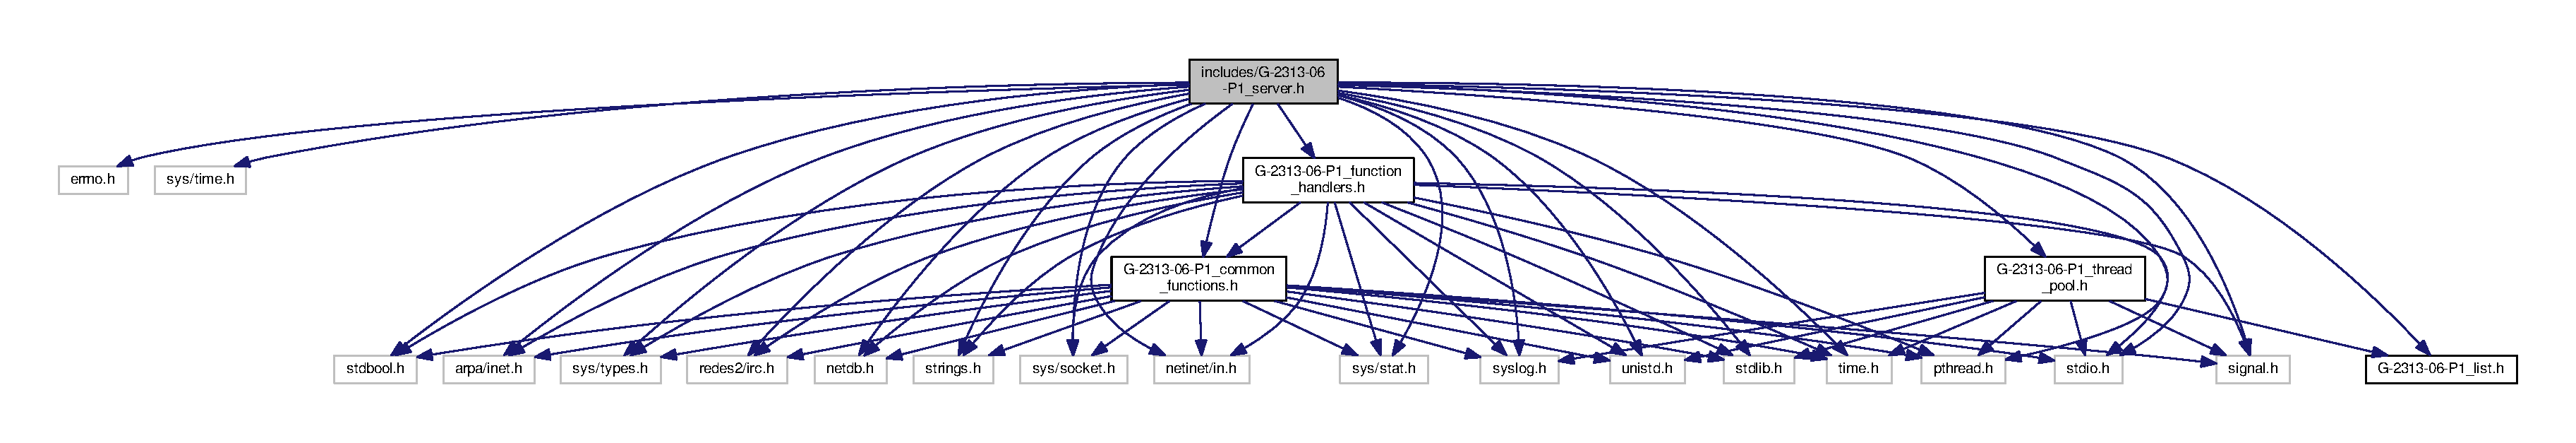
\includegraphics[width=350pt]{G-2313-06-P1__server_8h__incl}
\end{center}
\end{figure}
Gráfico de los archivos que directa o indirectamente incluyen a este archivo\+:\nopagebreak
\begin{figure}[H]
\begin{center}
\leavevmode
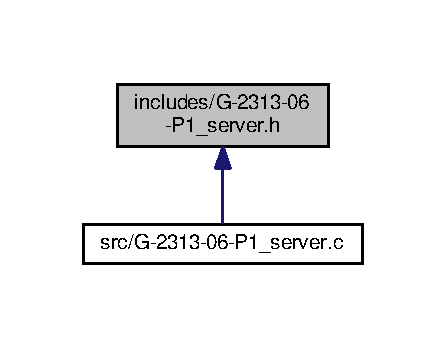
\includegraphics[width=214pt]{G-2313-06-P1__server_8h__dep__incl}
\end{center}
\end{figure}
\subsection*{\textquotesingle{}defines\textquotesingle{}}
\begin{DoxyCompactItemize}
\item 
\#define \hyperlink{G-2313-06-P1__server_8h_a80c7be19e867e55f90be3fa66cf65300}{M\+I\+N\+\_\+\+P\+O\+O\+L\+\_\+\+T\+H\+R\+E\+A\+D\+S}~3
\item 
\#define \hyperlink{G-2313-06-P1__server_8h_a053b7859476cc9867ec62c49e68d3fa1}{M\+A\+X\+\_\+\+C\+O\+N\+N\+E\+C\+T\+I\+O\+N\+S}~100
\item 
\#define \hyperlink{G-2313-06-P1__server_8h_ac42367fe5c999ec6650de83e9d72fe8c}{S\+E\+R\+V\+E\+R\+\_\+\+P\+O\+R\+T}~6667
\item 
\#define \hyperlink{G-2313-06-P1__server_8h_a97ed8e840fc4086fc86554e6d1277ca8}{C\+L\+I\+E\+N\+T\+\_\+\+M\+E\+S\+S\+A\+G\+E\+\_\+\+M\+A\+X\+S\+I\+Z\+E}~8096
\end{DoxyCompactItemize}
\subsection*{\textquotesingle{}typedefs\textquotesingle{}}
\begin{DoxyCompactItemize}
\item 
typedef void($\ast$ \hyperlink{G-2313-06-P1__server_8h_ae102cd0a63430b827183f70ce476a887}{Function\+Call\+Back}) (char $\ast$, int, char $\ast$, int $\ast$)
\end{DoxyCompactItemize}
\subsection*{Funciones}
\begin{DoxyCompactItemize}
\item 
int \hyperlink{G-2313-06-P1__server_8h_a85f40553bba77ada6c4329db58f68630}{server\+\_\+start} (void)
\item 
void \hyperlink{G-2313-06-P1__server_8h_ab201db206f26ab6fb26bb0e36dac4589}{server\+\_\+accept\+\_\+connection} (int socket\+\_\+id)
\item 
void $\ast$ \hyperlink{G-2313-06-P1__server_8h_a567404fb6edb67d9035359fef8e5acf3}{server\+\_\+start\+\_\+communication} (int connval)
\item 
void \hyperlink{G-2313-06-P1__server_8h_a0e947005d451a8f3bf3af01f54b59f11}{server\+\_\+exit} ()
\item 
void \hyperlink{G-2313-06-P1__server_8h_a775161328c3264fb8f96981f7a9c83ae}{server\+\_\+execute\+\_\+function} (long function\+Name, char $\ast$command, int desc, char $\ast$nick, int $\ast$register\+\_\+status)
\item 
int \hyperlink{G-2313-06-P1__server_8h_a64f1fffc5903ccf0350845cd21a95b6e}{server\+\_\+check\+\_\+socket\+\_\+status} (int socket\+\_\+desc)
\item 
void \hyperlink{G-2313-06-P1__server_8h_aa0e8000b12d9c52fc1e87847d00c9c47}{server\+\_\+daemon} ()
\item 
void \hyperlink{G-2313-06-P1__server_8h_a48d522cd984dc64ecd084f05416b1a94}{server\+\_\+start\+\_\+pool} ()
\end{DoxyCompactItemize}


\subsection{Documentación de los \textquotesingle{}defines\textquotesingle{}}
\hypertarget{G-2313-06-P1__server_8h_a97ed8e840fc4086fc86554e6d1277ca8}{}\index{G-\/2313-\/06-\/\+P1\+\_\+server.\+h@{G-\/2313-\/06-\/\+P1\+\_\+server.\+h}!C\+L\+I\+E\+N\+T\+\_\+\+M\+E\+S\+S\+A\+G\+E\+\_\+\+M\+A\+X\+S\+I\+Z\+E@{C\+L\+I\+E\+N\+T\+\_\+\+M\+E\+S\+S\+A\+G\+E\+\_\+\+M\+A\+X\+S\+I\+Z\+E}}
\index{C\+L\+I\+E\+N\+T\+\_\+\+M\+E\+S\+S\+A\+G\+E\+\_\+\+M\+A\+X\+S\+I\+Z\+E@{C\+L\+I\+E\+N\+T\+\_\+\+M\+E\+S\+S\+A\+G\+E\+\_\+\+M\+A\+X\+S\+I\+Z\+E}!G-\/2313-\/06-\/\+P1\+\_\+server.\+h@{G-\/2313-\/06-\/\+P1\+\_\+server.\+h}}
\subsubsection[{C\+L\+I\+E\+N\+T\+\_\+\+M\+E\+S\+S\+A\+G\+E\+\_\+\+M\+A\+X\+S\+I\+Z\+E}]{\setlength{\rightskip}{0pt plus 5cm}\#define C\+L\+I\+E\+N\+T\+\_\+\+M\+E\+S\+S\+A\+G\+E\+\_\+\+M\+A\+X\+S\+I\+Z\+E~8096}\label{G-2313-06-P1__server_8h_a97ed8e840fc4086fc86554e6d1277ca8}


Definición en la línea 29 del archivo G-\/2313-\/06-\/\+P1\+\_\+server.\+h.

\hypertarget{G-2313-06-P1__server_8h_a053b7859476cc9867ec62c49e68d3fa1}{}\index{G-\/2313-\/06-\/\+P1\+\_\+server.\+h@{G-\/2313-\/06-\/\+P1\+\_\+server.\+h}!M\+A\+X\+\_\+\+C\+O\+N\+N\+E\+C\+T\+I\+O\+N\+S@{M\+A\+X\+\_\+\+C\+O\+N\+N\+E\+C\+T\+I\+O\+N\+S}}
\index{M\+A\+X\+\_\+\+C\+O\+N\+N\+E\+C\+T\+I\+O\+N\+S@{M\+A\+X\+\_\+\+C\+O\+N\+N\+E\+C\+T\+I\+O\+N\+S}!G-\/2313-\/06-\/\+P1\+\_\+server.\+h@{G-\/2313-\/06-\/\+P1\+\_\+server.\+h}}
\subsubsection[{M\+A\+X\+\_\+\+C\+O\+N\+N\+E\+C\+T\+I\+O\+N\+S}]{\setlength{\rightskip}{0pt plus 5cm}\#define M\+A\+X\+\_\+\+C\+O\+N\+N\+E\+C\+T\+I\+O\+N\+S~100}\label{G-2313-06-P1__server_8h_a053b7859476cc9867ec62c49e68d3fa1}


Definición en la línea 27 del archivo G-\/2313-\/06-\/\+P1\+\_\+server.\+h.

\hypertarget{G-2313-06-P1__server_8h_a80c7be19e867e55f90be3fa66cf65300}{}\index{G-\/2313-\/06-\/\+P1\+\_\+server.\+h@{G-\/2313-\/06-\/\+P1\+\_\+server.\+h}!M\+I\+N\+\_\+\+P\+O\+O\+L\+\_\+\+T\+H\+R\+E\+A\+D\+S@{M\+I\+N\+\_\+\+P\+O\+O\+L\+\_\+\+T\+H\+R\+E\+A\+D\+S}}
\index{M\+I\+N\+\_\+\+P\+O\+O\+L\+\_\+\+T\+H\+R\+E\+A\+D\+S@{M\+I\+N\+\_\+\+P\+O\+O\+L\+\_\+\+T\+H\+R\+E\+A\+D\+S}!G-\/2313-\/06-\/\+P1\+\_\+server.\+h@{G-\/2313-\/06-\/\+P1\+\_\+server.\+h}}
\subsubsection[{M\+I\+N\+\_\+\+P\+O\+O\+L\+\_\+\+T\+H\+R\+E\+A\+D\+S}]{\setlength{\rightskip}{0pt plus 5cm}\#define M\+I\+N\+\_\+\+P\+O\+O\+L\+\_\+\+T\+H\+R\+E\+A\+D\+S~3}\label{G-2313-06-P1__server_8h_a80c7be19e867e55f90be3fa66cf65300}


Definición en la línea 26 del archivo G-\/2313-\/06-\/\+P1\+\_\+server.\+h.

\hypertarget{G-2313-06-P1__server_8h_ac42367fe5c999ec6650de83e9d72fe8c}{}\index{G-\/2313-\/06-\/\+P1\+\_\+server.\+h@{G-\/2313-\/06-\/\+P1\+\_\+server.\+h}!S\+E\+R\+V\+E\+R\+\_\+\+P\+O\+R\+T@{S\+E\+R\+V\+E\+R\+\_\+\+P\+O\+R\+T}}
\index{S\+E\+R\+V\+E\+R\+\_\+\+P\+O\+R\+T@{S\+E\+R\+V\+E\+R\+\_\+\+P\+O\+R\+T}!G-\/2313-\/06-\/\+P1\+\_\+server.\+h@{G-\/2313-\/06-\/\+P1\+\_\+server.\+h}}
\subsubsection[{S\+E\+R\+V\+E\+R\+\_\+\+P\+O\+R\+T}]{\setlength{\rightskip}{0pt plus 5cm}\#define S\+E\+R\+V\+E\+R\+\_\+\+P\+O\+R\+T~6667}\label{G-2313-06-P1__server_8h_ac42367fe5c999ec6650de83e9d72fe8c}


Definición en la línea 28 del archivo G-\/2313-\/06-\/\+P1\+\_\+server.\+h.



\subsection{Documentación de los \textquotesingle{}typedefs\textquotesingle{}}
\hypertarget{G-2313-06-P1__server_8h_ae102cd0a63430b827183f70ce476a887}{}\index{G-\/2313-\/06-\/\+P1\+\_\+server.\+h@{G-\/2313-\/06-\/\+P1\+\_\+server.\+h}!Function\+Call\+Back@{Function\+Call\+Back}}
\index{Function\+Call\+Back@{Function\+Call\+Back}!G-\/2313-\/06-\/\+P1\+\_\+server.\+h@{G-\/2313-\/06-\/\+P1\+\_\+server.\+h}}
\subsubsection[{Function\+Call\+Back}]{\setlength{\rightskip}{0pt plus 5cm}typedef void($\ast$ Function\+Call\+Back) (char $\ast$, int, char $\ast$, int $\ast$)}\label{G-2313-06-P1__server_8h_ae102cd0a63430b827183f70ce476a887}


Definición en la línea 41 del archivo G-\/2313-\/06-\/\+P1\+\_\+server.\+h.



\subsection{Documentación de las funciones}
\hypertarget{G-2313-06-P1__server_8h_ab201db206f26ab6fb26bb0e36dac4589}{}\index{G-\/2313-\/06-\/\+P1\+\_\+server.\+h@{G-\/2313-\/06-\/\+P1\+\_\+server.\+h}!server\+\_\+accept\+\_\+connection@{server\+\_\+accept\+\_\+connection}}
\index{server\+\_\+accept\+\_\+connection@{server\+\_\+accept\+\_\+connection}!G-\/2313-\/06-\/\+P1\+\_\+server.\+h@{G-\/2313-\/06-\/\+P1\+\_\+server.\+h}}
\subsubsection[{server\+\_\+accept\+\_\+connection}]{\setlength{\rightskip}{0pt plus 5cm}void server\+\_\+accept\+\_\+connection (
\begin{DoxyParamCaption}
\item[{int}]{socket\+\_\+id}
\end{DoxyParamCaption}
)}\label{G-2313-06-P1__server_8h_ab201db206f26ab6fb26bb0e36dac4589}


Definición en la línea 171 del archivo G-\/2313-\/06-\/\+P1\+\_\+server.\+c.

\hypertarget{G-2313-06-P1__server_8h_a64f1fffc5903ccf0350845cd21a95b6e}{}\index{G-\/2313-\/06-\/\+P1\+\_\+server.\+h@{G-\/2313-\/06-\/\+P1\+\_\+server.\+h}!server\+\_\+check\+\_\+socket\+\_\+status@{server\+\_\+check\+\_\+socket\+\_\+status}}
\index{server\+\_\+check\+\_\+socket\+\_\+status@{server\+\_\+check\+\_\+socket\+\_\+status}!G-\/2313-\/06-\/\+P1\+\_\+server.\+h@{G-\/2313-\/06-\/\+P1\+\_\+server.\+h}}
\subsubsection[{server\+\_\+check\+\_\+socket\+\_\+status}]{\setlength{\rightskip}{0pt plus 5cm}int server\+\_\+check\+\_\+socket\+\_\+status (
\begin{DoxyParamCaption}
\item[{int}]{socket\+\_\+desc}
\end{DoxyParamCaption}
)}\label{G-2313-06-P1__server_8h_a64f1fffc5903ccf0350845cd21a95b6e}


Definición en la línea 473 del archivo G-\/2313-\/06-\/\+P1\+\_\+server.\+c.

\hypertarget{G-2313-06-P1__server_8h_aa0e8000b12d9c52fc1e87847d00c9c47}{}\index{G-\/2313-\/06-\/\+P1\+\_\+server.\+h@{G-\/2313-\/06-\/\+P1\+\_\+server.\+h}!server\+\_\+daemon@{server\+\_\+daemon}}
\index{server\+\_\+daemon@{server\+\_\+daemon}!G-\/2313-\/06-\/\+P1\+\_\+server.\+h@{G-\/2313-\/06-\/\+P1\+\_\+server.\+h}}
\subsubsection[{server\+\_\+daemon}]{\setlength{\rightskip}{0pt plus 5cm}void server\+\_\+daemon (
\begin{DoxyParamCaption}
{}
\end{DoxyParamCaption}
)}\label{G-2313-06-P1__server_8h_aa0e8000b12d9c52fc1e87847d00c9c47}


Definición en la línea 518 del archivo G-\/2313-\/06-\/\+P1\+\_\+server.\+c.

\hypertarget{G-2313-06-P1__server_8h_a775161328c3264fb8f96981f7a9c83ae}{}\index{G-\/2313-\/06-\/\+P1\+\_\+server.\+h@{G-\/2313-\/06-\/\+P1\+\_\+server.\+h}!server\+\_\+execute\+\_\+function@{server\+\_\+execute\+\_\+function}}
\index{server\+\_\+execute\+\_\+function@{server\+\_\+execute\+\_\+function}!G-\/2313-\/06-\/\+P1\+\_\+server.\+h@{G-\/2313-\/06-\/\+P1\+\_\+server.\+h}}
\subsubsection[{server\+\_\+execute\+\_\+function}]{\setlength{\rightskip}{0pt plus 5cm}void server\+\_\+execute\+\_\+function (
\begin{DoxyParamCaption}
\item[{long}]{function\+Name, }
\item[{char $\ast$}]{command, }
\item[{int}]{desc, }
\item[{char $\ast$}]{nick, }
\item[{int $\ast$}]{register\+\_\+status}
\end{DoxyParamCaption}
)}\label{G-2313-06-P1__server_8h_a775161328c3264fb8f96981f7a9c83ae}


Definición en la línea 368 del archivo G-\/2313-\/06-\/\+P1\+\_\+server.\+c.

\hypertarget{G-2313-06-P1__server_8h_a0e947005d451a8f3bf3af01f54b59f11}{}\index{G-\/2313-\/06-\/\+P1\+\_\+server.\+h@{G-\/2313-\/06-\/\+P1\+\_\+server.\+h}!server\+\_\+exit@{server\+\_\+exit}}
\index{server\+\_\+exit@{server\+\_\+exit}!G-\/2313-\/06-\/\+P1\+\_\+server.\+h@{G-\/2313-\/06-\/\+P1\+\_\+server.\+h}}
\subsubsection[{server\+\_\+exit}]{\setlength{\rightskip}{0pt plus 5cm}void server\+\_\+exit (
\begin{DoxyParamCaption}
{}
\end{DoxyParamCaption}
)}\label{G-2313-06-P1__server_8h_a0e947005d451a8f3bf3af01f54b59f11}


Definición en la línea 436 del archivo G-\/2313-\/06-\/\+P1\+\_\+server.\+c.

\hypertarget{G-2313-06-P1__server_8h_a85f40553bba77ada6c4329db58f68630}{}\index{G-\/2313-\/06-\/\+P1\+\_\+server.\+h@{G-\/2313-\/06-\/\+P1\+\_\+server.\+h}!server\+\_\+start@{server\+\_\+start}}
\index{server\+\_\+start@{server\+\_\+start}!G-\/2313-\/06-\/\+P1\+\_\+server.\+h@{G-\/2313-\/06-\/\+P1\+\_\+server.\+h}}
\subsubsection[{server\+\_\+start}]{\setlength{\rightskip}{0pt plus 5cm}int server\+\_\+start (
\begin{DoxyParamCaption}
\item[{void}]{}
\end{DoxyParamCaption}
)}\label{G-2313-06-P1__server_8h_a85f40553bba77ada6c4329db58f68630}


Definición en la línea 101 del archivo G-\/2313-\/06-\/\+P1\+\_\+server.\+c.

\hypertarget{G-2313-06-P1__server_8h_a567404fb6edb67d9035359fef8e5acf3}{}\index{G-\/2313-\/06-\/\+P1\+\_\+server.\+h@{G-\/2313-\/06-\/\+P1\+\_\+server.\+h}!server\+\_\+start\+\_\+communication@{server\+\_\+start\+\_\+communication}}
\index{server\+\_\+start\+\_\+communication@{server\+\_\+start\+\_\+communication}!G-\/2313-\/06-\/\+P1\+\_\+server.\+h@{G-\/2313-\/06-\/\+P1\+\_\+server.\+h}}
\subsubsection[{server\+\_\+start\+\_\+communication}]{\setlength{\rightskip}{0pt plus 5cm}void$\ast$ server\+\_\+start\+\_\+communication (
\begin{DoxyParamCaption}
\item[{int}]{connval}
\end{DoxyParamCaption}
)}\label{G-2313-06-P1__server_8h_a567404fb6edb67d9035359fef8e5acf3}


Definición en la línea 252 del archivo G-\/2313-\/06-\/\+P1\+\_\+server.\+c.

\hypertarget{G-2313-06-P1__server_8h_a48d522cd984dc64ecd084f05416b1a94}{}\index{G-\/2313-\/06-\/\+P1\+\_\+server.\+h@{G-\/2313-\/06-\/\+P1\+\_\+server.\+h}!server\+\_\+start\+\_\+pool@{server\+\_\+start\+\_\+pool}}
\index{server\+\_\+start\+\_\+pool@{server\+\_\+start\+\_\+pool}!G-\/2313-\/06-\/\+P1\+\_\+server.\+h@{G-\/2313-\/06-\/\+P1\+\_\+server.\+h}}
\subsubsection[{server\+\_\+start\+\_\+pool}]{\setlength{\rightskip}{0pt plus 5cm}void server\+\_\+start\+\_\+pool (
\begin{DoxyParamCaption}
{}
\end{DoxyParamCaption}
)}\label{G-2313-06-P1__server_8h_a48d522cd984dc64ecd084f05416b1a94}


Definición en la línea 558 del archivo G-\/2313-\/06-\/\+P1\+\_\+server.\+c.


\hypertarget{G-2313-06-P1__thread__pool_8h}{}\section{Referencia del Archivo includes/\+G-\/2313-\/06-\/\+P1\+\_\+thread\+\_\+pool.h}
\label{G-2313-06-P1__thread__pool_8h}\index{includes/\+G-\/2313-\/06-\/\+P1\+\_\+thread\+\_\+pool.\+h@{includes/\+G-\/2313-\/06-\/\+P1\+\_\+thread\+\_\+pool.\+h}}
{\ttfamily \#include $<$pthread.\+h$>$}\\*
{\ttfamily \#include $<$stdlib.\+h$>$}\\*
{\ttfamily \#include $<$stdio.\+h$>$}\\*
{\ttfamily \#include $<$time.\+h$>$}\\*
{\ttfamily \#include $<$syslog.\+h$>$}\\*
{\ttfamily \#include $<$signal.\+h$>$}\\*
{\ttfamily \#include $<$unistd.\+h$>$}\\*
{\ttfamily \#include \char`\"{}G-\/2313-\/06-\/\+P1\+\_\+list.\+h\char`\"{}}\\*
Dependencia gráfica adjunta para G-\/2313-\/06-\/\+P1\+\_\+thread\+\_\+pool.h\+:\nopagebreak
\begin{figure}[H]
\begin{center}
\leavevmode
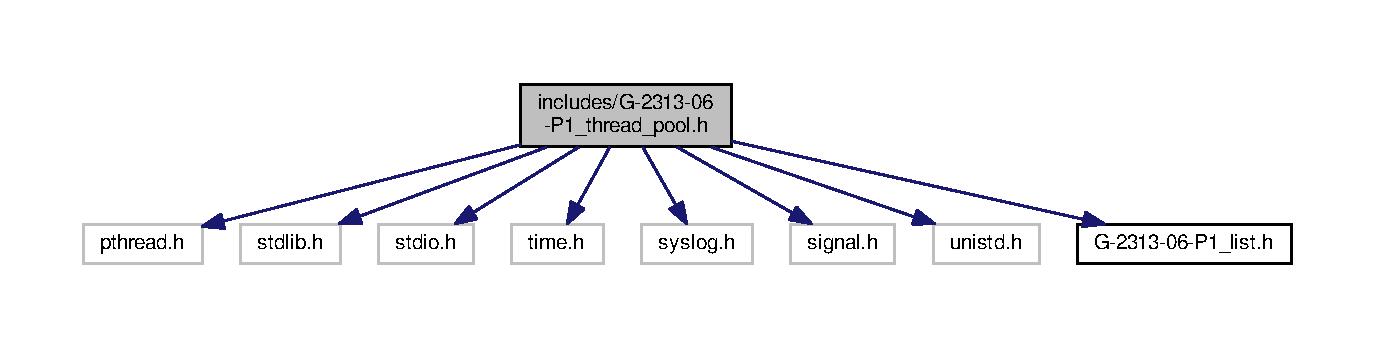
\includegraphics[width=350pt]{G-2313-06-P1__thread__pool_8h__incl}
\end{center}
\end{figure}
Gráfico de los archivos que directa o indirectamente incluyen a este archivo\+:\nopagebreak
\begin{figure}[H]
\begin{center}
\leavevmode
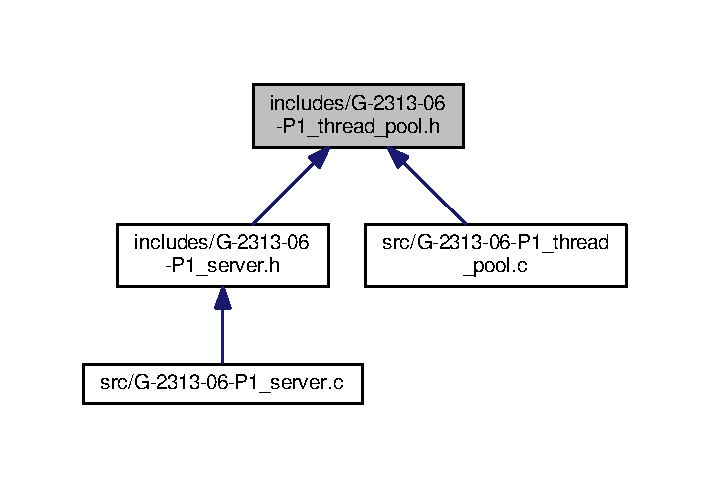
\includegraphics[width=341pt]{G-2313-06-P1__thread__pool_8h__dep__incl}
\end{center}
\end{figure}
\subsection*{Clases}
\begin{DoxyCompactItemize}
\item 
struct \hyperlink{structtask__t}{task\+\_\+t}
\item 
struct \hyperlink{structthread__t}{thread\+\_\+t}
\item 
struct \hyperlink{structthread__pool__t}{thread\+\_\+pool\+\_\+t}
\item 
struct \hyperlink{structthread__args}{thread\+\_\+args}
\end{DoxyCompactItemize}
\subsection*{\textquotesingle{}defines\textquotesingle{}}
\begin{DoxyCompactItemize}
\item 
\#define \hyperlink{G-2313-06-P1__thread__pool_8h_a1d5f9a0a6439db9d27573f4ea768e03a}{T\+H\+R\+E\+A\+D\+\_\+\+P\+O\+O\+L\+\_\+\+M\+A\+X\+\_\+\+T\+H\+R\+E\+A\+D\+S}~100
\item 
\#define \hyperlink{G-2313-06-P1__thread__pool_8h_a2dddf10750568983fb5e8793f467e170}{T\+H\+R\+E\+A\+D\+\_\+\+P\+O\+O\+L\+\_\+\+M\+I\+N\+\_\+\+T\+H\+R\+E\+A\+D\+S}~10
\item 
\#define \hyperlink{G-2313-06-P1__thread__pool_8h_a91780ed988c2db43eb70b7106cee217b}{T\+H\+R\+E\+A\+D\+\_\+\+S\+T\+A\+T\+E\+\_\+\+B\+U\+S\+Y}~0\+X1
\item 
\#define \hyperlink{G-2313-06-P1__thread__pool_8h_a7fb00c8fb812a4f9a1c08e22a95104a1}{T\+H\+R\+E\+A\+D\+\_\+\+S\+T\+A\+T\+E\+\_\+\+I\+D\+L\+E}~0x2
\item 
\#define \hyperlink{G-2313-06-P1__thread__pool_8h_acef14a4788dacf3640cf28745cf49726}{T\+H\+R\+E\+A\+D\+\_\+\+S\+T\+O\+P\+P\+I\+N\+G}~0x1
\item 
\#define \hyperlink{G-2313-06-P1__thread__pool_8h_a9c22e7eceaed2a27b40b3bd043c1d057}{T\+H\+R\+E\+A\+D\+\_\+\+R\+U\+N\+N\+I\+N\+G}~0x2
\item 
\#define \hyperlink{G-2313-06-P1__thread__pool_8h_a9466670765f7653fc75437eb55c472f3}{T\+H\+R\+E\+A\+D\+\_\+\+I\+D\+L\+E\+\_\+\+L\+E\+V\+E\+L}~0.\+2
\item 
\#define \hyperlink{G-2313-06-P1__thread__pool_8h_a09199434ab101700c051a235cf740f30}{T\+H\+R\+E\+A\+D\+\_\+\+B\+U\+S\+Y\+\_\+\+L\+E\+V\+E\+L}~0.\+8
\item 
\#define \hyperlink{G-2313-06-P1__thread__pool_8h_a562492e441dc328fba8a344c7206758a}{M\+A\+S\+T\+E\+R\+\_\+\+I\+N\+T\+E\+R\+V\+A\+L}~10
\end{DoxyCompactItemize}
\subsection*{\textquotesingle{}typedefs\textquotesingle{}}
\begin{DoxyCompactItemize}
\item 
typedef struct \hyperlink{structtask__t}{task\+\_\+t} \hyperlink{G-2313-06-P1__thread__pool_8h_a989e278a815d7ada960572a3e9fad896}{task\+\_\+t}
\item 
typedef struct \hyperlink{structthread__t}{thread\+\_\+t} \hyperlink{G-2313-06-P1__thread__pool_8h_a6e84f6599234bedf30a8b88f56e8fd48}{thread\+\_\+t}
\item 
typedef struct \hyperlink{structthread__pool__t}{thread\+\_\+pool\+\_\+t} \hyperlink{G-2313-06-P1__thread__pool_8h_a5f14d1f0d9a94d2e45b01104049529eb}{thread\+\_\+pool\+\_\+t}
\item 
typedef struct \hyperlink{structthread__args}{thread\+\_\+args} \hyperlink{G-2313-06-P1__thread__pool_8h_ae7684b0001f8477707ef97e117e09d31}{thread\+\_\+args}
\end{DoxyCompactItemize}
\subsection*{Funciones}
\begin{DoxyCompactItemize}
\item 
\hyperlink{structthread__pool__t}{thread\+\_\+pool\+\_\+t} $\ast$ \hyperlink{G-2313-06-P1__thread__pool_8h_ae4c7364510f378011559c4eb6078e3ea}{thread\+\_\+pool\+\_\+create} (int size)
\item 
void \hyperlink{G-2313-06-P1__thread__pool_8h_a46b14e66a9466a68fa4f67a2e08e81fd}{thread\+\_\+pool\+\_\+delete} (\hyperlink{structthread__pool__t}{thread\+\_\+pool\+\_\+t} $\ast$p)
\item 
int \hyperlink{G-2313-06-P1__thread__pool_8h_aa9d4a7977fc5b5b534b60415a3aa7311}{thread\+\_\+pool\+\_\+init} (\hyperlink{structthread__pool__t}{thread\+\_\+pool\+\_\+t} $\ast$)
\item 
int \hyperlink{G-2313-06-P1__thread__pool_8h_a6f48d348c6ba66b0f85b6c0cb6d89737}{thread\+\_\+pool\+\_\+init\+\_\+internal} (\hyperlink{structthread__pool__t}{thread\+\_\+pool\+\_\+t} $\ast$, double low\+\_\+level, double high\+\_\+level, int master\+\_\+interval)
\item 
void $\ast$ \hyperlink{G-2313-06-P1__thread__pool_8h_a54703c23462be974a5e2511247921922}{master\+\_\+callback} (void $\ast$arg)
\item 
void $\ast$ \hyperlink{G-2313-06-P1__thread__pool_8h_a4ef081fb21acd34e0e2492a9f290b6a3}{worker\+\_\+callback} (void $\ast$arg)
\item 
\hyperlink{structthread__t}{thread\+\_\+t} $\ast$ \hyperlink{G-2313-06-P1__thread__pool_8h_a920e51bce81dfc069372dd87935db55e}{thread\+\_\+create} (void)
\item 
int \hyperlink{G-2313-06-P1__thread__pool_8h_a4820a76ce58452afff503b4ae218be5c}{thread\+\_\+add} (\hyperlink{structthread__pool__t}{thread\+\_\+pool\+\_\+t} $\ast$, \hyperlink{structthread__t}{thread\+\_\+t} $\ast$)
\item 
void \hyperlink{G-2313-06-P1__thread__pool_8h_aa2094f3613d648102f798506b1e86347}{thread\+\_\+del\+\_\+internal} (\hyperlink{structthread__pool__t}{thread\+\_\+pool\+\_\+t} $\ast$, \hyperlink{structthread__t}{thread\+\_\+t} $\ast$, int)
\item 
void \hyperlink{G-2313-06-P1__thread__pool_8h_a95970a6ee2f49963fc3fe7aefa677194}{thread\+\_\+del} (\hyperlink{structthread__t}{thread\+\_\+t} $\ast$t)
\item 
\hyperlink{structtask__t}{task\+\_\+t} $\ast$ \hyperlink{G-2313-06-P1__thread__pool_8h_afa05870619a7e753d41b8135b8514a2c}{task\+\_\+create} (void)
\item 
void \hyperlink{G-2313-06-P1__thread__pool_8h_a7241a5097164175e730f610eaad0aa5a}{task\+\_\+init} (\hyperlink{structtask__t}{task\+\_\+t} $\ast$, void $\ast$($\ast$)(int), int arg)
\item 
void \hyperlink{G-2313-06-P1__thread__pool_8h_a113acb632971a3b3acd2cda2c4620bb3}{task\+\_\+add} (\hyperlink{structthread__pool__t}{thread\+\_\+pool\+\_\+t} $\ast$, \hyperlink{structtask__t}{task\+\_\+t} $\ast$)
\end{DoxyCompactItemize}


\subsection{Documentación de los \textquotesingle{}defines\textquotesingle{}}
\hypertarget{G-2313-06-P1__thread__pool_8h_a562492e441dc328fba8a344c7206758a}{}\index{G-\/2313-\/06-\/\+P1\+\_\+thread\+\_\+pool.\+h@{G-\/2313-\/06-\/\+P1\+\_\+thread\+\_\+pool.\+h}!M\+A\+S\+T\+E\+R\+\_\+\+I\+N\+T\+E\+R\+V\+A\+L@{M\+A\+S\+T\+E\+R\+\_\+\+I\+N\+T\+E\+R\+V\+A\+L}}
\index{M\+A\+S\+T\+E\+R\+\_\+\+I\+N\+T\+E\+R\+V\+A\+L@{M\+A\+S\+T\+E\+R\+\_\+\+I\+N\+T\+E\+R\+V\+A\+L}!G-\/2313-\/06-\/\+P1\+\_\+thread\+\_\+pool.\+h@{G-\/2313-\/06-\/\+P1\+\_\+thread\+\_\+pool.\+h}}
\subsubsection[{M\+A\+S\+T\+E\+R\+\_\+\+I\+N\+T\+E\+R\+V\+A\+L}]{\setlength{\rightskip}{0pt plus 5cm}\#define M\+A\+S\+T\+E\+R\+\_\+\+I\+N\+T\+E\+R\+V\+A\+L~10}\label{G-2313-06-P1__thread__pool_8h_a562492e441dc328fba8a344c7206758a}


Definición en la línea 25 del archivo G-\/2313-\/06-\/\+P1\+\_\+thread\+\_\+pool.\+h.

\hypertarget{G-2313-06-P1__thread__pool_8h_a09199434ab101700c051a235cf740f30}{}\index{G-\/2313-\/06-\/\+P1\+\_\+thread\+\_\+pool.\+h@{G-\/2313-\/06-\/\+P1\+\_\+thread\+\_\+pool.\+h}!T\+H\+R\+E\+A\+D\+\_\+\+B\+U\+S\+Y\+\_\+\+L\+E\+V\+E\+L@{T\+H\+R\+E\+A\+D\+\_\+\+B\+U\+S\+Y\+\_\+\+L\+E\+V\+E\+L}}
\index{T\+H\+R\+E\+A\+D\+\_\+\+B\+U\+S\+Y\+\_\+\+L\+E\+V\+E\+L@{T\+H\+R\+E\+A\+D\+\_\+\+B\+U\+S\+Y\+\_\+\+L\+E\+V\+E\+L}!G-\/2313-\/06-\/\+P1\+\_\+thread\+\_\+pool.\+h@{G-\/2313-\/06-\/\+P1\+\_\+thread\+\_\+pool.\+h}}
\subsubsection[{T\+H\+R\+E\+A\+D\+\_\+\+B\+U\+S\+Y\+\_\+\+L\+E\+V\+E\+L}]{\setlength{\rightskip}{0pt plus 5cm}\#define T\+H\+R\+E\+A\+D\+\_\+\+B\+U\+S\+Y\+\_\+\+L\+E\+V\+E\+L~0.\+8}\label{G-2313-06-P1__thread__pool_8h_a09199434ab101700c051a235cf740f30}


Definición en la línea 23 del archivo G-\/2313-\/06-\/\+P1\+\_\+thread\+\_\+pool.\+h.

\hypertarget{G-2313-06-P1__thread__pool_8h_a9466670765f7653fc75437eb55c472f3}{}\index{G-\/2313-\/06-\/\+P1\+\_\+thread\+\_\+pool.\+h@{G-\/2313-\/06-\/\+P1\+\_\+thread\+\_\+pool.\+h}!T\+H\+R\+E\+A\+D\+\_\+\+I\+D\+L\+E\+\_\+\+L\+E\+V\+E\+L@{T\+H\+R\+E\+A\+D\+\_\+\+I\+D\+L\+E\+\_\+\+L\+E\+V\+E\+L}}
\index{T\+H\+R\+E\+A\+D\+\_\+\+I\+D\+L\+E\+\_\+\+L\+E\+V\+E\+L@{T\+H\+R\+E\+A\+D\+\_\+\+I\+D\+L\+E\+\_\+\+L\+E\+V\+E\+L}!G-\/2313-\/06-\/\+P1\+\_\+thread\+\_\+pool.\+h@{G-\/2313-\/06-\/\+P1\+\_\+thread\+\_\+pool.\+h}}
\subsubsection[{T\+H\+R\+E\+A\+D\+\_\+\+I\+D\+L\+E\+\_\+\+L\+E\+V\+E\+L}]{\setlength{\rightskip}{0pt plus 5cm}\#define T\+H\+R\+E\+A\+D\+\_\+\+I\+D\+L\+E\+\_\+\+L\+E\+V\+E\+L~0.\+2}\label{G-2313-06-P1__thread__pool_8h_a9466670765f7653fc75437eb55c472f3}


Definición en la línea 22 del archivo G-\/2313-\/06-\/\+P1\+\_\+thread\+\_\+pool.\+h.

\hypertarget{G-2313-06-P1__thread__pool_8h_a1d5f9a0a6439db9d27573f4ea768e03a}{}\index{G-\/2313-\/06-\/\+P1\+\_\+thread\+\_\+pool.\+h@{G-\/2313-\/06-\/\+P1\+\_\+thread\+\_\+pool.\+h}!T\+H\+R\+E\+A\+D\+\_\+\+P\+O\+O\+L\+\_\+\+M\+A\+X\+\_\+\+T\+H\+R\+E\+A\+D\+S@{T\+H\+R\+E\+A\+D\+\_\+\+P\+O\+O\+L\+\_\+\+M\+A\+X\+\_\+\+T\+H\+R\+E\+A\+D\+S}}
\index{T\+H\+R\+E\+A\+D\+\_\+\+P\+O\+O\+L\+\_\+\+M\+A\+X\+\_\+\+T\+H\+R\+E\+A\+D\+S@{T\+H\+R\+E\+A\+D\+\_\+\+P\+O\+O\+L\+\_\+\+M\+A\+X\+\_\+\+T\+H\+R\+E\+A\+D\+S}!G-\/2313-\/06-\/\+P1\+\_\+thread\+\_\+pool.\+h@{G-\/2313-\/06-\/\+P1\+\_\+thread\+\_\+pool.\+h}}
\subsubsection[{T\+H\+R\+E\+A\+D\+\_\+\+P\+O\+O\+L\+\_\+\+M\+A\+X\+\_\+\+T\+H\+R\+E\+A\+D\+S}]{\setlength{\rightskip}{0pt plus 5cm}\#define T\+H\+R\+E\+A\+D\+\_\+\+P\+O\+O\+L\+\_\+\+M\+A\+X\+\_\+\+T\+H\+R\+E\+A\+D\+S~100}\label{G-2313-06-P1__thread__pool_8h_a1d5f9a0a6439db9d27573f4ea768e03a}


Definición en la línea 13 del archivo G-\/2313-\/06-\/\+P1\+\_\+thread\+\_\+pool.\+h.

\hypertarget{G-2313-06-P1__thread__pool_8h_a2dddf10750568983fb5e8793f467e170}{}\index{G-\/2313-\/06-\/\+P1\+\_\+thread\+\_\+pool.\+h@{G-\/2313-\/06-\/\+P1\+\_\+thread\+\_\+pool.\+h}!T\+H\+R\+E\+A\+D\+\_\+\+P\+O\+O\+L\+\_\+\+M\+I\+N\+\_\+\+T\+H\+R\+E\+A\+D\+S@{T\+H\+R\+E\+A\+D\+\_\+\+P\+O\+O\+L\+\_\+\+M\+I\+N\+\_\+\+T\+H\+R\+E\+A\+D\+S}}
\index{T\+H\+R\+E\+A\+D\+\_\+\+P\+O\+O\+L\+\_\+\+M\+I\+N\+\_\+\+T\+H\+R\+E\+A\+D\+S@{T\+H\+R\+E\+A\+D\+\_\+\+P\+O\+O\+L\+\_\+\+M\+I\+N\+\_\+\+T\+H\+R\+E\+A\+D\+S}!G-\/2313-\/06-\/\+P1\+\_\+thread\+\_\+pool.\+h@{G-\/2313-\/06-\/\+P1\+\_\+thread\+\_\+pool.\+h}}
\subsubsection[{T\+H\+R\+E\+A\+D\+\_\+\+P\+O\+O\+L\+\_\+\+M\+I\+N\+\_\+\+T\+H\+R\+E\+A\+D\+S}]{\setlength{\rightskip}{0pt plus 5cm}\#define T\+H\+R\+E\+A\+D\+\_\+\+P\+O\+O\+L\+\_\+\+M\+I\+N\+\_\+\+T\+H\+R\+E\+A\+D\+S~10}\label{G-2313-06-P1__thread__pool_8h_a2dddf10750568983fb5e8793f467e170}


Definición en la línea 14 del archivo G-\/2313-\/06-\/\+P1\+\_\+thread\+\_\+pool.\+h.

\hypertarget{G-2313-06-P1__thread__pool_8h_a9c22e7eceaed2a27b40b3bd043c1d057}{}\index{G-\/2313-\/06-\/\+P1\+\_\+thread\+\_\+pool.\+h@{G-\/2313-\/06-\/\+P1\+\_\+thread\+\_\+pool.\+h}!T\+H\+R\+E\+A\+D\+\_\+\+R\+U\+N\+N\+I\+N\+G@{T\+H\+R\+E\+A\+D\+\_\+\+R\+U\+N\+N\+I\+N\+G}}
\index{T\+H\+R\+E\+A\+D\+\_\+\+R\+U\+N\+N\+I\+N\+G@{T\+H\+R\+E\+A\+D\+\_\+\+R\+U\+N\+N\+I\+N\+G}!G-\/2313-\/06-\/\+P1\+\_\+thread\+\_\+pool.\+h@{G-\/2313-\/06-\/\+P1\+\_\+thread\+\_\+pool.\+h}}
\subsubsection[{T\+H\+R\+E\+A\+D\+\_\+\+R\+U\+N\+N\+I\+N\+G}]{\setlength{\rightskip}{0pt plus 5cm}\#define T\+H\+R\+E\+A\+D\+\_\+\+R\+U\+N\+N\+I\+N\+G~0x2}\label{G-2313-06-P1__thread__pool_8h_a9c22e7eceaed2a27b40b3bd043c1d057}


Definición en la línea 20 del archivo G-\/2313-\/06-\/\+P1\+\_\+thread\+\_\+pool.\+h.

\hypertarget{G-2313-06-P1__thread__pool_8h_a91780ed988c2db43eb70b7106cee217b}{}\index{G-\/2313-\/06-\/\+P1\+\_\+thread\+\_\+pool.\+h@{G-\/2313-\/06-\/\+P1\+\_\+thread\+\_\+pool.\+h}!T\+H\+R\+E\+A\+D\+\_\+\+S\+T\+A\+T\+E\+\_\+\+B\+U\+S\+Y@{T\+H\+R\+E\+A\+D\+\_\+\+S\+T\+A\+T\+E\+\_\+\+B\+U\+S\+Y}}
\index{T\+H\+R\+E\+A\+D\+\_\+\+S\+T\+A\+T\+E\+\_\+\+B\+U\+S\+Y@{T\+H\+R\+E\+A\+D\+\_\+\+S\+T\+A\+T\+E\+\_\+\+B\+U\+S\+Y}!G-\/2313-\/06-\/\+P1\+\_\+thread\+\_\+pool.\+h@{G-\/2313-\/06-\/\+P1\+\_\+thread\+\_\+pool.\+h}}
\subsubsection[{T\+H\+R\+E\+A\+D\+\_\+\+S\+T\+A\+T\+E\+\_\+\+B\+U\+S\+Y}]{\setlength{\rightskip}{0pt plus 5cm}\#define T\+H\+R\+E\+A\+D\+\_\+\+S\+T\+A\+T\+E\+\_\+\+B\+U\+S\+Y~0\+X1}\label{G-2313-06-P1__thread__pool_8h_a91780ed988c2db43eb70b7106cee217b}


Definición en la línea 16 del archivo G-\/2313-\/06-\/\+P1\+\_\+thread\+\_\+pool.\+h.

\hypertarget{G-2313-06-P1__thread__pool_8h_a7fb00c8fb812a4f9a1c08e22a95104a1}{}\index{G-\/2313-\/06-\/\+P1\+\_\+thread\+\_\+pool.\+h@{G-\/2313-\/06-\/\+P1\+\_\+thread\+\_\+pool.\+h}!T\+H\+R\+E\+A\+D\+\_\+\+S\+T\+A\+T\+E\+\_\+\+I\+D\+L\+E@{T\+H\+R\+E\+A\+D\+\_\+\+S\+T\+A\+T\+E\+\_\+\+I\+D\+L\+E}}
\index{T\+H\+R\+E\+A\+D\+\_\+\+S\+T\+A\+T\+E\+\_\+\+I\+D\+L\+E@{T\+H\+R\+E\+A\+D\+\_\+\+S\+T\+A\+T\+E\+\_\+\+I\+D\+L\+E}!G-\/2313-\/06-\/\+P1\+\_\+thread\+\_\+pool.\+h@{G-\/2313-\/06-\/\+P1\+\_\+thread\+\_\+pool.\+h}}
\subsubsection[{T\+H\+R\+E\+A\+D\+\_\+\+S\+T\+A\+T\+E\+\_\+\+I\+D\+L\+E}]{\setlength{\rightskip}{0pt plus 5cm}\#define T\+H\+R\+E\+A\+D\+\_\+\+S\+T\+A\+T\+E\+\_\+\+I\+D\+L\+E~0x2}\label{G-2313-06-P1__thread__pool_8h_a7fb00c8fb812a4f9a1c08e22a95104a1}


Definición en la línea 17 del archivo G-\/2313-\/06-\/\+P1\+\_\+thread\+\_\+pool.\+h.

\hypertarget{G-2313-06-P1__thread__pool_8h_acef14a4788dacf3640cf28745cf49726}{}\index{G-\/2313-\/06-\/\+P1\+\_\+thread\+\_\+pool.\+h@{G-\/2313-\/06-\/\+P1\+\_\+thread\+\_\+pool.\+h}!T\+H\+R\+E\+A\+D\+\_\+\+S\+T\+O\+P\+P\+I\+N\+G@{T\+H\+R\+E\+A\+D\+\_\+\+S\+T\+O\+P\+P\+I\+N\+G}}
\index{T\+H\+R\+E\+A\+D\+\_\+\+S\+T\+O\+P\+P\+I\+N\+G@{T\+H\+R\+E\+A\+D\+\_\+\+S\+T\+O\+P\+P\+I\+N\+G}!G-\/2313-\/06-\/\+P1\+\_\+thread\+\_\+pool.\+h@{G-\/2313-\/06-\/\+P1\+\_\+thread\+\_\+pool.\+h}}
\subsubsection[{T\+H\+R\+E\+A\+D\+\_\+\+S\+T\+O\+P\+P\+I\+N\+G}]{\setlength{\rightskip}{0pt plus 5cm}\#define T\+H\+R\+E\+A\+D\+\_\+\+S\+T\+O\+P\+P\+I\+N\+G~0x1}\label{G-2313-06-P1__thread__pool_8h_acef14a4788dacf3640cf28745cf49726}


Definición en la línea 19 del archivo G-\/2313-\/06-\/\+P1\+\_\+thread\+\_\+pool.\+h.



\subsection{Documentación de los \textquotesingle{}typedefs\textquotesingle{}}
\hypertarget{G-2313-06-P1__thread__pool_8h_a989e278a815d7ada960572a3e9fad896}{}\index{G-\/2313-\/06-\/\+P1\+\_\+thread\+\_\+pool.\+h@{G-\/2313-\/06-\/\+P1\+\_\+thread\+\_\+pool.\+h}!task\+\_\+t@{task\+\_\+t}}
\index{task\+\_\+t@{task\+\_\+t}!G-\/2313-\/06-\/\+P1\+\_\+thread\+\_\+pool.\+h@{G-\/2313-\/06-\/\+P1\+\_\+thread\+\_\+pool.\+h}}
\subsubsection[{task\+\_\+t}]{\setlength{\rightskip}{0pt plus 5cm}typedef struct {\bf task\+\_\+t} {\bf task\+\_\+t}}\label{G-2313-06-P1__thread__pool_8h_a989e278a815d7ada960572a3e9fad896}
\hypertarget{G-2313-06-P1__thread__pool_8h_ae7684b0001f8477707ef97e117e09d31}{}\index{G-\/2313-\/06-\/\+P1\+\_\+thread\+\_\+pool.\+h@{G-\/2313-\/06-\/\+P1\+\_\+thread\+\_\+pool.\+h}!thread\+\_\+args@{thread\+\_\+args}}
\index{thread\+\_\+args@{thread\+\_\+args}!G-\/2313-\/06-\/\+P1\+\_\+thread\+\_\+pool.\+h@{G-\/2313-\/06-\/\+P1\+\_\+thread\+\_\+pool.\+h}}
\subsubsection[{thread\+\_\+args}]{\setlength{\rightskip}{0pt plus 5cm}typedef struct {\bf thread\+\_\+args} {\bf thread\+\_\+args}}\label{G-2313-06-P1__thread__pool_8h_ae7684b0001f8477707ef97e117e09d31}
\hypertarget{G-2313-06-P1__thread__pool_8h_a5f14d1f0d9a94d2e45b01104049529eb}{}\index{G-\/2313-\/06-\/\+P1\+\_\+thread\+\_\+pool.\+h@{G-\/2313-\/06-\/\+P1\+\_\+thread\+\_\+pool.\+h}!thread\+\_\+pool\+\_\+t@{thread\+\_\+pool\+\_\+t}}
\index{thread\+\_\+pool\+\_\+t@{thread\+\_\+pool\+\_\+t}!G-\/2313-\/06-\/\+P1\+\_\+thread\+\_\+pool.\+h@{G-\/2313-\/06-\/\+P1\+\_\+thread\+\_\+pool.\+h}}
\subsubsection[{thread\+\_\+pool\+\_\+t}]{\setlength{\rightskip}{0pt plus 5cm}typedef struct {\bf thread\+\_\+pool\+\_\+t} {\bf thread\+\_\+pool\+\_\+t}}\label{G-2313-06-P1__thread__pool_8h_a5f14d1f0d9a94d2e45b01104049529eb}
\hypertarget{G-2313-06-P1__thread__pool_8h_a6e84f6599234bedf30a8b88f56e8fd48}{}\index{G-\/2313-\/06-\/\+P1\+\_\+thread\+\_\+pool.\+h@{G-\/2313-\/06-\/\+P1\+\_\+thread\+\_\+pool.\+h}!thread\+\_\+t@{thread\+\_\+t}}
\index{thread\+\_\+t@{thread\+\_\+t}!G-\/2313-\/06-\/\+P1\+\_\+thread\+\_\+pool.\+h@{G-\/2313-\/06-\/\+P1\+\_\+thread\+\_\+pool.\+h}}
\subsubsection[{thread\+\_\+t}]{\setlength{\rightskip}{0pt plus 5cm}typedef struct {\bf thread\+\_\+t} {\bf thread\+\_\+t}}\label{G-2313-06-P1__thread__pool_8h_a6e84f6599234bedf30a8b88f56e8fd48}


\subsection{Documentación de las funciones}
\hypertarget{G-2313-06-P1__thread__pool_8h_a54703c23462be974a5e2511247921922}{}\index{G-\/2313-\/06-\/\+P1\+\_\+thread\+\_\+pool.\+h@{G-\/2313-\/06-\/\+P1\+\_\+thread\+\_\+pool.\+h}!master\+\_\+callback@{master\+\_\+callback}}
\index{master\+\_\+callback@{master\+\_\+callback}!G-\/2313-\/06-\/\+P1\+\_\+thread\+\_\+pool.\+h@{G-\/2313-\/06-\/\+P1\+\_\+thread\+\_\+pool.\+h}}
\subsubsection[{master\+\_\+callback}]{\setlength{\rightskip}{0pt plus 5cm}void$\ast$ master\+\_\+callback (
\begin{DoxyParamCaption}
\item[{void $\ast$}]{arg}
\end{DoxyParamCaption}
)}\label{G-2313-06-P1__thread__pool_8h_a54703c23462be974a5e2511247921922}


Definición en la línea 222 del archivo G-\/2313-\/06-\/\+P1\+\_\+thread\+\_\+pool.\+c.

\hypertarget{G-2313-06-P1__thread__pool_8h_a113acb632971a3b3acd2cda2c4620bb3}{}\index{G-\/2313-\/06-\/\+P1\+\_\+thread\+\_\+pool.\+h@{G-\/2313-\/06-\/\+P1\+\_\+thread\+\_\+pool.\+h}!task\+\_\+add@{task\+\_\+add}}
\index{task\+\_\+add@{task\+\_\+add}!G-\/2313-\/06-\/\+P1\+\_\+thread\+\_\+pool.\+h@{G-\/2313-\/06-\/\+P1\+\_\+thread\+\_\+pool.\+h}}
\subsubsection[{task\+\_\+add}]{\setlength{\rightskip}{0pt plus 5cm}void task\+\_\+add (
\begin{DoxyParamCaption}
\item[{{\bf thread\+\_\+pool\+\_\+t} $\ast$}]{, }
\item[{{\bf task\+\_\+t} $\ast$}]{}
\end{DoxyParamCaption}
)}\label{G-2313-06-P1__thread__pool_8h_a113acb632971a3b3acd2cda2c4620bb3}


Definición en la línea 277 del archivo G-\/2313-\/06-\/\+P1\+\_\+thread\+\_\+pool.\+c.

\hypertarget{G-2313-06-P1__thread__pool_8h_afa05870619a7e753d41b8135b8514a2c}{}\index{G-\/2313-\/06-\/\+P1\+\_\+thread\+\_\+pool.\+h@{G-\/2313-\/06-\/\+P1\+\_\+thread\+\_\+pool.\+h}!task\+\_\+create@{task\+\_\+create}}
\index{task\+\_\+create@{task\+\_\+create}!G-\/2313-\/06-\/\+P1\+\_\+thread\+\_\+pool.\+h@{G-\/2313-\/06-\/\+P1\+\_\+thread\+\_\+pool.\+h}}
\subsubsection[{task\+\_\+create}]{\setlength{\rightskip}{0pt plus 5cm}{\bf task\+\_\+t}$\ast$ task\+\_\+create (
\begin{DoxyParamCaption}
\item[{void}]{}
\end{DoxyParamCaption}
)}\label{G-2313-06-P1__thread__pool_8h_afa05870619a7e753d41b8135b8514a2c}


Definición en la línea 259 del archivo G-\/2313-\/06-\/\+P1\+\_\+thread\+\_\+pool.\+c.

\hypertarget{G-2313-06-P1__thread__pool_8h_a7241a5097164175e730f610eaad0aa5a}{}\index{G-\/2313-\/06-\/\+P1\+\_\+thread\+\_\+pool.\+h@{G-\/2313-\/06-\/\+P1\+\_\+thread\+\_\+pool.\+h}!task\+\_\+init@{task\+\_\+init}}
\index{task\+\_\+init@{task\+\_\+init}!G-\/2313-\/06-\/\+P1\+\_\+thread\+\_\+pool.\+h@{G-\/2313-\/06-\/\+P1\+\_\+thread\+\_\+pool.\+h}}
\subsubsection[{task\+\_\+init}]{\setlength{\rightskip}{0pt plus 5cm}void task\+\_\+init (
\begin{DoxyParamCaption}
\item[{{\bf task\+\_\+t} $\ast$}]{, }
\item[{void $\ast$}]{$\ast$)(int, }
\item[{int}]{arg}
\end{DoxyParamCaption}
)}\label{G-2313-06-P1__thread__pool_8h_a7241a5097164175e730f610eaad0aa5a}
\hypertarget{G-2313-06-P1__thread__pool_8h_a4820a76ce58452afff503b4ae218be5c}{}\index{G-\/2313-\/06-\/\+P1\+\_\+thread\+\_\+pool.\+h@{G-\/2313-\/06-\/\+P1\+\_\+thread\+\_\+pool.\+h}!thread\+\_\+add@{thread\+\_\+add}}
\index{thread\+\_\+add@{thread\+\_\+add}!G-\/2313-\/06-\/\+P1\+\_\+thread\+\_\+pool.\+h@{G-\/2313-\/06-\/\+P1\+\_\+thread\+\_\+pool.\+h}}
\subsubsection[{thread\+\_\+add}]{\setlength{\rightskip}{0pt plus 5cm}int thread\+\_\+add (
\begin{DoxyParamCaption}
\item[{{\bf thread\+\_\+pool\+\_\+t} $\ast$}]{, }
\item[{{\bf thread\+\_\+t} $\ast$}]{}
\end{DoxyParamCaption}
)}\label{G-2313-06-P1__thread__pool_8h_a4820a76ce58452afff503b4ae218be5c}


Definición en la línea 121 del archivo G-\/2313-\/06-\/\+P1\+\_\+thread\+\_\+pool.\+c.

\hypertarget{G-2313-06-P1__thread__pool_8h_a920e51bce81dfc069372dd87935db55e}{}\index{G-\/2313-\/06-\/\+P1\+\_\+thread\+\_\+pool.\+h@{G-\/2313-\/06-\/\+P1\+\_\+thread\+\_\+pool.\+h}!thread\+\_\+create@{thread\+\_\+create}}
\index{thread\+\_\+create@{thread\+\_\+create}!G-\/2313-\/06-\/\+P1\+\_\+thread\+\_\+pool.\+h@{G-\/2313-\/06-\/\+P1\+\_\+thread\+\_\+pool.\+h}}
\subsubsection[{thread\+\_\+create}]{\setlength{\rightskip}{0pt plus 5cm}{\bf thread\+\_\+t}$\ast$ thread\+\_\+create (
\begin{DoxyParamCaption}
\item[{void}]{}
\end{DoxyParamCaption}
)}\label{G-2313-06-P1__thread__pool_8h_a920e51bce81dfc069372dd87935db55e}


Definición en la línea 109 del archivo G-\/2313-\/06-\/\+P1\+\_\+thread\+\_\+pool.\+c.

\hypertarget{G-2313-06-P1__thread__pool_8h_a95970a6ee2f49963fc3fe7aefa677194}{}\index{G-\/2313-\/06-\/\+P1\+\_\+thread\+\_\+pool.\+h@{G-\/2313-\/06-\/\+P1\+\_\+thread\+\_\+pool.\+h}!thread\+\_\+del@{thread\+\_\+del}}
\index{thread\+\_\+del@{thread\+\_\+del}!G-\/2313-\/06-\/\+P1\+\_\+thread\+\_\+pool.\+h@{G-\/2313-\/06-\/\+P1\+\_\+thread\+\_\+pool.\+h}}
\subsubsection[{thread\+\_\+del}]{\setlength{\rightskip}{0pt plus 5cm}void thread\+\_\+del (
\begin{DoxyParamCaption}
\item[{{\bf thread\+\_\+t} $\ast$}]{t}
\end{DoxyParamCaption}
)}\label{G-2313-06-P1__thread__pool_8h_a95970a6ee2f49963fc3fe7aefa677194}


Definición en la línea 152 del archivo G-\/2313-\/06-\/\+P1\+\_\+thread\+\_\+pool.\+c.

\hypertarget{G-2313-06-P1__thread__pool_8h_aa2094f3613d648102f798506b1e86347}{}\index{G-\/2313-\/06-\/\+P1\+\_\+thread\+\_\+pool.\+h@{G-\/2313-\/06-\/\+P1\+\_\+thread\+\_\+pool.\+h}!thread\+\_\+del\+\_\+internal@{thread\+\_\+del\+\_\+internal}}
\index{thread\+\_\+del\+\_\+internal@{thread\+\_\+del\+\_\+internal}!G-\/2313-\/06-\/\+P1\+\_\+thread\+\_\+pool.\+h@{G-\/2313-\/06-\/\+P1\+\_\+thread\+\_\+pool.\+h}}
\subsubsection[{thread\+\_\+del\+\_\+internal}]{\setlength{\rightskip}{0pt plus 5cm}void thread\+\_\+del\+\_\+internal (
\begin{DoxyParamCaption}
\item[{{\bf thread\+\_\+pool\+\_\+t} $\ast$}]{, }
\item[{{\bf thread\+\_\+t} $\ast$}]{, }
\item[{int}]{}
\end{DoxyParamCaption}
)}\label{G-2313-06-P1__thread__pool_8h_aa2094f3613d648102f798506b1e86347}


Definición en la línea 159 del archivo G-\/2313-\/06-\/\+P1\+\_\+thread\+\_\+pool.\+c.

\hypertarget{G-2313-06-P1__thread__pool_8h_ae4c7364510f378011559c4eb6078e3ea}{}\index{G-\/2313-\/06-\/\+P1\+\_\+thread\+\_\+pool.\+h@{G-\/2313-\/06-\/\+P1\+\_\+thread\+\_\+pool.\+h}!thread\+\_\+pool\+\_\+create@{thread\+\_\+pool\+\_\+create}}
\index{thread\+\_\+pool\+\_\+create@{thread\+\_\+pool\+\_\+create}!G-\/2313-\/06-\/\+P1\+\_\+thread\+\_\+pool.\+h@{G-\/2313-\/06-\/\+P1\+\_\+thread\+\_\+pool.\+h}}
\subsubsection[{thread\+\_\+pool\+\_\+create}]{\setlength{\rightskip}{0pt plus 5cm}{\bf thread\+\_\+pool\+\_\+t}$\ast$ thread\+\_\+pool\+\_\+create (
\begin{DoxyParamCaption}
\item[{int}]{size}
\end{DoxyParamCaption}
)}\label{G-2313-06-P1__thread__pool_8h_ae4c7364510f378011559c4eb6078e3ea}


Definición en la línea 3 del archivo G-\/2313-\/06-\/\+P1\+\_\+thread\+\_\+pool.\+c.

\hypertarget{G-2313-06-P1__thread__pool_8h_a46b14e66a9466a68fa4f67a2e08e81fd}{}\index{G-\/2313-\/06-\/\+P1\+\_\+thread\+\_\+pool.\+h@{G-\/2313-\/06-\/\+P1\+\_\+thread\+\_\+pool.\+h}!thread\+\_\+pool\+\_\+delete@{thread\+\_\+pool\+\_\+delete}}
\index{thread\+\_\+pool\+\_\+delete@{thread\+\_\+pool\+\_\+delete}!G-\/2313-\/06-\/\+P1\+\_\+thread\+\_\+pool.\+h@{G-\/2313-\/06-\/\+P1\+\_\+thread\+\_\+pool.\+h}}
\subsubsection[{thread\+\_\+pool\+\_\+delete}]{\setlength{\rightskip}{0pt plus 5cm}void thread\+\_\+pool\+\_\+delete (
\begin{DoxyParamCaption}
\item[{{\bf thread\+\_\+pool\+\_\+t} $\ast$}]{p}
\end{DoxyParamCaption}
)}\label{G-2313-06-P1__thread__pool_8h_a46b14e66a9466a68fa4f67a2e08e81fd}


Definición en la línea 27 del archivo G-\/2313-\/06-\/\+P1\+\_\+thread\+\_\+pool.\+c.

\hypertarget{G-2313-06-P1__thread__pool_8h_aa9d4a7977fc5b5b534b60415a3aa7311}{}\index{G-\/2313-\/06-\/\+P1\+\_\+thread\+\_\+pool.\+h@{G-\/2313-\/06-\/\+P1\+\_\+thread\+\_\+pool.\+h}!thread\+\_\+pool\+\_\+init@{thread\+\_\+pool\+\_\+init}}
\index{thread\+\_\+pool\+\_\+init@{thread\+\_\+pool\+\_\+init}!G-\/2313-\/06-\/\+P1\+\_\+thread\+\_\+pool.\+h@{G-\/2313-\/06-\/\+P1\+\_\+thread\+\_\+pool.\+h}}
\subsubsection[{thread\+\_\+pool\+\_\+init}]{\setlength{\rightskip}{0pt plus 5cm}int thread\+\_\+pool\+\_\+init (
\begin{DoxyParamCaption}
\item[{{\bf thread\+\_\+pool\+\_\+t} $\ast$}]{}
\end{DoxyParamCaption}
)}\label{G-2313-06-P1__thread__pool_8h_aa9d4a7977fc5b5b534b60415a3aa7311}


Definición en la línea 58 del archivo G-\/2313-\/06-\/\+P1\+\_\+thread\+\_\+pool.\+c.

\hypertarget{G-2313-06-P1__thread__pool_8h_a6f48d348c6ba66b0f85b6c0cb6d89737}{}\index{G-\/2313-\/06-\/\+P1\+\_\+thread\+\_\+pool.\+h@{G-\/2313-\/06-\/\+P1\+\_\+thread\+\_\+pool.\+h}!thread\+\_\+pool\+\_\+init\+\_\+internal@{thread\+\_\+pool\+\_\+init\+\_\+internal}}
\index{thread\+\_\+pool\+\_\+init\+\_\+internal@{thread\+\_\+pool\+\_\+init\+\_\+internal}!G-\/2313-\/06-\/\+P1\+\_\+thread\+\_\+pool.\+h@{G-\/2313-\/06-\/\+P1\+\_\+thread\+\_\+pool.\+h}}
\subsubsection[{thread\+\_\+pool\+\_\+init\+\_\+internal}]{\setlength{\rightskip}{0pt plus 5cm}int thread\+\_\+pool\+\_\+init\+\_\+internal (
\begin{DoxyParamCaption}
\item[{{\bf thread\+\_\+pool\+\_\+t} $\ast$}]{, }
\item[{double}]{low\+\_\+level, }
\item[{double}]{high\+\_\+level, }
\item[{int}]{master\+\_\+interval}
\end{DoxyParamCaption}
)}\label{G-2313-06-P1__thread__pool_8h_a6f48d348c6ba66b0f85b6c0cb6d89737}


Definición en la línea 64 del archivo G-\/2313-\/06-\/\+P1\+\_\+thread\+\_\+pool.\+c.

\hypertarget{G-2313-06-P1__thread__pool_8h_a4ef081fb21acd34e0e2492a9f290b6a3}{}\index{G-\/2313-\/06-\/\+P1\+\_\+thread\+\_\+pool.\+h@{G-\/2313-\/06-\/\+P1\+\_\+thread\+\_\+pool.\+h}!worker\+\_\+callback@{worker\+\_\+callback}}
\index{worker\+\_\+callback@{worker\+\_\+callback}!G-\/2313-\/06-\/\+P1\+\_\+thread\+\_\+pool.\+h@{G-\/2313-\/06-\/\+P1\+\_\+thread\+\_\+pool.\+h}}
\subsubsection[{worker\+\_\+callback}]{\setlength{\rightskip}{0pt plus 5cm}void$\ast$ worker\+\_\+callback (
\begin{DoxyParamCaption}
\item[{void $\ast$}]{arg}
\end{DoxyParamCaption}
)}\label{G-2313-06-P1__thread__pool_8h_a4ef081fb21acd34e0e2492a9f290b6a3}


Definición en la línea 171 del archivo G-\/2313-\/06-\/\+P1\+\_\+thread\+\_\+pool.\+c.


\hypertarget{G-2313-06-P1__common__functions_8c}{}\section{Referencia del Archivo src/\+G-\/2313-\/06-\/\+P1\+\_\+common\+\_\+functions.c}
\label{G-2313-06-P1__common__functions_8c}\index{src/\+G-\/2313-\/06-\/\+P1\+\_\+common\+\_\+functions.\+c@{src/\+G-\/2313-\/06-\/\+P1\+\_\+common\+\_\+functions.\+c}}
{\ttfamily \#include \char`\"{}../includes/\+G-\/2313-\/06-\/\+P1\+\_\+common\+\_\+functions.\+h\char`\"{}}\\*
Dependencia gráfica adjunta para G-\/2313-\/06-\/\+P1\+\_\+common\+\_\+functions.c\+:\nopagebreak
\begin{figure}[H]
\begin{center}
\leavevmode
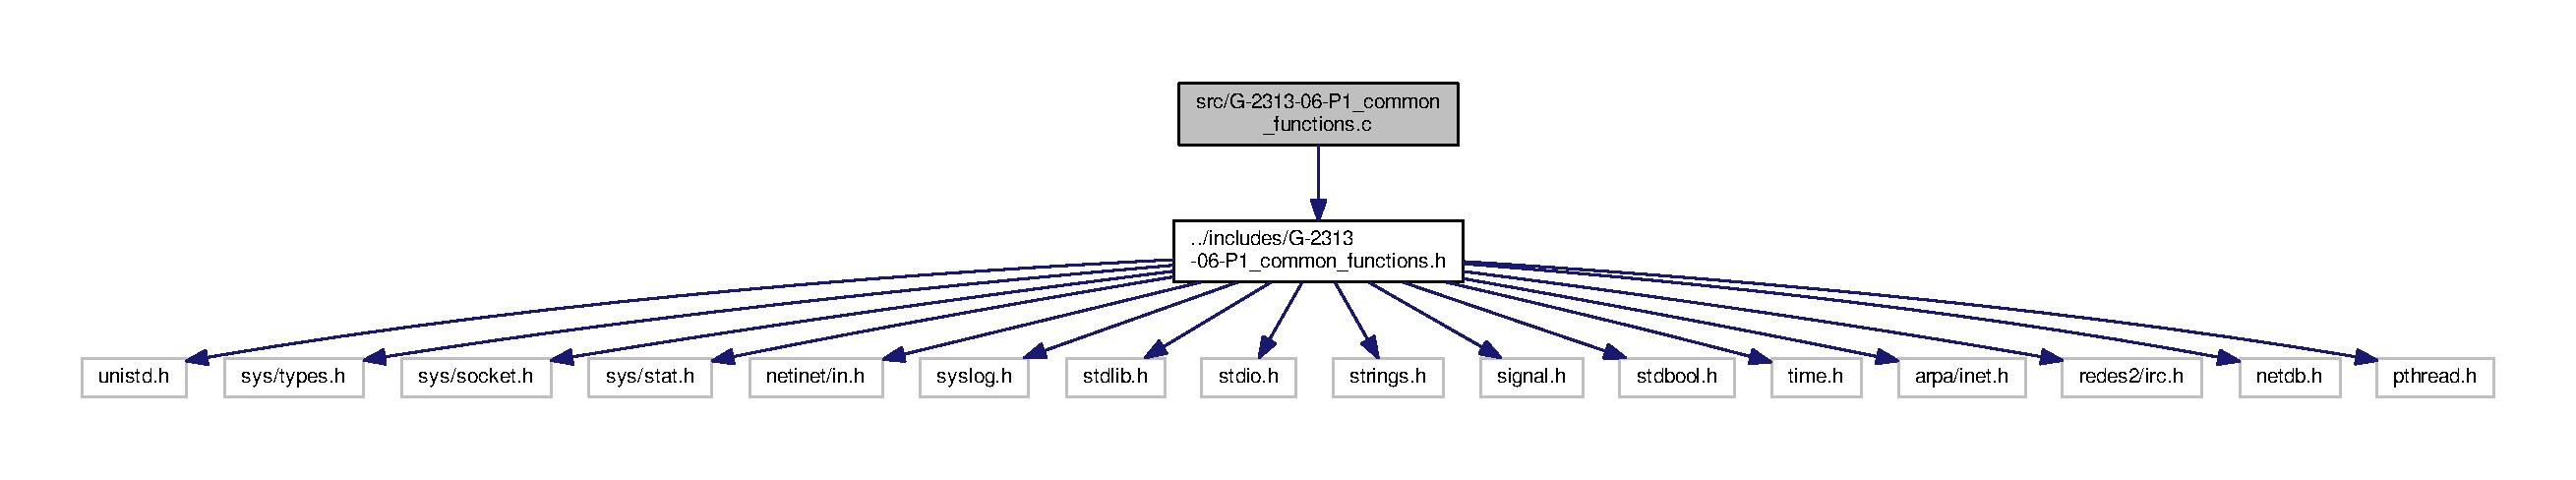
\includegraphics[width=350pt]{G-2313-06-P1__common__functions_8c__incl}
\end{center}
\end{figure}
\subsection*{Funciones}
\begin{DoxyCompactItemize}
\item 
int \hyperlink{G-2313-06-P1__common__functions_8c_a61cca6f1a1adeb81f722ecc2ff35aab5}{server\+\_\+users\+\_\+find\+\_\+by\+\_\+nick} (char $\ast$data)
\item 
int \hyperlink{G-2313-06-P1__common__functions_8c_a485e68f66db6ae4b7297d99c32afe30a}{server\+\_\+users\+\_\+find\+\_\+by\+\_\+socket} (int sockdesc)
\item 
int \hyperlink{G-2313-06-P1__common__functions_8c_a875ae5278d95716b494b26f96cf4ae6e}{server\+\_\+channels\+\_\+find\+\_\+by\+\_\+name} (char $\ast$channel)
\item 
int \hyperlink{G-2313-06-P1__common__functions_8c_ae8a282d9cdfc8187b8e74e368bc56d92}{server\+\_\+channels\+\_\+update\+\_\+nick} (char $\ast$nick\+\_\+old, char $\ast$nick\+\_\+new)
\item 
int \hyperlink{G-2313-06-P1__common__functions_8c_af9aeb632d55a4cbbe842ab97001b5128}{server\+\_\+channels\+\_\+update\+\_\+away} (char $\ast$nick, char $\ast$away)
\item 
char $\ast$ \hyperlink{G-2313-06-P1__common__functions_8c_a230bf24ab7ae18d2e81ebc1d3575a6ad}{server\+\_\+return\+\_\+user} (char $\ast$nick)
\end{DoxyCompactItemize}


\subsection{Documentación de las funciones}
\hypertarget{G-2313-06-P1__common__functions_8c_a875ae5278d95716b494b26f96cf4ae6e}{}\index{G-\/2313-\/06-\/\+P1\+\_\+common\+\_\+functions.\+c@{G-\/2313-\/06-\/\+P1\+\_\+common\+\_\+functions.\+c}!server\+\_\+channels\+\_\+find\+\_\+by\+\_\+name@{server\+\_\+channels\+\_\+find\+\_\+by\+\_\+name}}
\index{server\+\_\+channels\+\_\+find\+\_\+by\+\_\+name@{server\+\_\+channels\+\_\+find\+\_\+by\+\_\+name}!G-\/2313-\/06-\/\+P1\+\_\+common\+\_\+functions.\+c@{G-\/2313-\/06-\/\+P1\+\_\+common\+\_\+functions.\+c}}
\subsubsection[{server\+\_\+channels\+\_\+find\+\_\+by\+\_\+name}]{\setlength{\rightskip}{0pt plus 5cm}int server\+\_\+channels\+\_\+find\+\_\+by\+\_\+name (
\begin{DoxyParamCaption}
\item[{char $\ast$}]{channel}
\end{DoxyParamCaption}
)}\label{G-2313-06-P1__common__functions_8c_a875ae5278d95716b494b26f96cf4ae6e}


Definición en la línea 178 del archivo G-\/2313-\/06-\/\+P1\+\_\+common\+\_\+functions.\+c.

\hypertarget{G-2313-06-P1__common__functions_8c_af9aeb632d55a4cbbe842ab97001b5128}{}\index{G-\/2313-\/06-\/\+P1\+\_\+common\+\_\+functions.\+c@{G-\/2313-\/06-\/\+P1\+\_\+common\+\_\+functions.\+c}!server\+\_\+channels\+\_\+update\+\_\+away@{server\+\_\+channels\+\_\+update\+\_\+away}}
\index{server\+\_\+channels\+\_\+update\+\_\+away@{server\+\_\+channels\+\_\+update\+\_\+away}!G-\/2313-\/06-\/\+P1\+\_\+common\+\_\+functions.\+c@{G-\/2313-\/06-\/\+P1\+\_\+common\+\_\+functions.\+c}}
\subsubsection[{server\+\_\+channels\+\_\+update\+\_\+away}]{\setlength{\rightskip}{0pt plus 5cm}int server\+\_\+channels\+\_\+update\+\_\+away (
\begin{DoxyParamCaption}
\item[{char $\ast$}]{nick, }
\item[{char $\ast$}]{away}
\end{DoxyParamCaption}
)}\label{G-2313-06-P1__common__functions_8c_af9aeb632d55a4cbbe842ab97001b5128}


Definición en la línea 275 del archivo G-\/2313-\/06-\/\+P1\+\_\+common\+\_\+functions.\+c.

\hypertarget{G-2313-06-P1__common__functions_8c_ae8a282d9cdfc8187b8e74e368bc56d92}{}\index{G-\/2313-\/06-\/\+P1\+\_\+common\+\_\+functions.\+c@{G-\/2313-\/06-\/\+P1\+\_\+common\+\_\+functions.\+c}!server\+\_\+channels\+\_\+update\+\_\+nick@{server\+\_\+channels\+\_\+update\+\_\+nick}}
\index{server\+\_\+channels\+\_\+update\+\_\+nick@{server\+\_\+channels\+\_\+update\+\_\+nick}!G-\/2313-\/06-\/\+P1\+\_\+common\+\_\+functions.\+c@{G-\/2313-\/06-\/\+P1\+\_\+common\+\_\+functions.\+c}}
\subsubsection[{server\+\_\+channels\+\_\+update\+\_\+nick}]{\setlength{\rightskip}{0pt plus 5cm}int server\+\_\+channels\+\_\+update\+\_\+nick (
\begin{DoxyParamCaption}
\item[{char $\ast$}]{nick\+\_\+old, }
\item[{char $\ast$}]{nick\+\_\+new}
\end{DoxyParamCaption}
)}\label{G-2313-06-P1__common__functions_8c_ae8a282d9cdfc8187b8e74e368bc56d92}


Definición en la línea 221 del archivo G-\/2313-\/06-\/\+P1\+\_\+common\+\_\+functions.\+c.

\hypertarget{G-2313-06-P1__common__functions_8c_a230bf24ab7ae18d2e81ebc1d3575a6ad}{}\index{G-\/2313-\/06-\/\+P1\+\_\+common\+\_\+functions.\+c@{G-\/2313-\/06-\/\+P1\+\_\+common\+\_\+functions.\+c}!server\+\_\+return\+\_\+user@{server\+\_\+return\+\_\+user}}
\index{server\+\_\+return\+\_\+user@{server\+\_\+return\+\_\+user}!G-\/2313-\/06-\/\+P1\+\_\+common\+\_\+functions.\+c@{G-\/2313-\/06-\/\+P1\+\_\+common\+\_\+functions.\+c}}
\subsubsection[{server\+\_\+return\+\_\+user}]{\setlength{\rightskip}{0pt plus 5cm}char$\ast$ server\+\_\+return\+\_\+user (
\begin{DoxyParamCaption}
\item[{char $\ast$}]{nick}
\end{DoxyParamCaption}
)}\label{G-2313-06-P1__common__functions_8c_a230bf24ab7ae18d2e81ebc1d3575a6ad}


Definición en la línea 327 del archivo G-\/2313-\/06-\/\+P1\+\_\+common\+\_\+functions.\+c.

\hypertarget{G-2313-06-P1__common__functions_8c_a61cca6f1a1adeb81f722ecc2ff35aab5}{}\index{G-\/2313-\/06-\/\+P1\+\_\+common\+\_\+functions.\+c@{G-\/2313-\/06-\/\+P1\+\_\+common\+\_\+functions.\+c}!server\+\_\+users\+\_\+find\+\_\+by\+\_\+nick@{server\+\_\+users\+\_\+find\+\_\+by\+\_\+nick}}
\index{server\+\_\+users\+\_\+find\+\_\+by\+\_\+nick@{server\+\_\+users\+\_\+find\+\_\+by\+\_\+nick}!G-\/2313-\/06-\/\+P1\+\_\+common\+\_\+functions.\+c@{G-\/2313-\/06-\/\+P1\+\_\+common\+\_\+functions.\+c}}
\subsubsection[{server\+\_\+users\+\_\+find\+\_\+by\+\_\+nick}]{\setlength{\rightskip}{0pt plus 5cm}int server\+\_\+users\+\_\+find\+\_\+by\+\_\+nick (
\begin{DoxyParamCaption}
\item[{char $\ast$}]{data}
\end{DoxyParamCaption}
)}\label{G-2313-06-P1__common__functions_8c_a61cca6f1a1adeb81f722ecc2ff35aab5}


Definición en la línea 52 del archivo G-\/2313-\/06-\/\+P1\+\_\+common\+\_\+functions.\+c.

\hypertarget{G-2313-06-P1__common__functions_8c_a485e68f66db6ae4b7297d99c32afe30a}{}\index{G-\/2313-\/06-\/\+P1\+\_\+common\+\_\+functions.\+c@{G-\/2313-\/06-\/\+P1\+\_\+common\+\_\+functions.\+c}!server\+\_\+users\+\_\+find\+\_\+by\+\_\+socket@{server\+\_\+users\+\_\+find\+\_\+by\+\_\+socket}}
\index{server\+\_\+users\+\_\+find\+\_\+by\+\_\+socket@{server\+\_\+users\+\_\+find\+\_\+by\+\_\+socket}!G-\/2313-\/06-\/\+P1\+\_\+common\+\_\+functions.\+c@{G-\/2313-\/06-\/\+P1\+\_\+common\+\_\+functions.\+c}}
\subsubsection[{server\+\_\+users\+\_\+find\+\_\+by\+\_\+socket}]{\setlength{\rightskip}{0pt plus 5cm}int server\+\_\+users\+\_\+find\+\_\+by\+\_\+socket (
\begin{DoxyParamCaption}
\item[{int}]{sockdesc}
\end{DoxyParamCaption}
)}\label{G-2313-06-P1__common__functions_8c_a485e68f66db6ae4b7297d99c32afe30a}


Definición en la línea 113 del archivo G-\/2313-\/06-\/\+P1\+\_\+common\+\_\+functions.\+c.


\hypertarget{G-2313-06-P1__function__handlers_8c}{}\section{Referencia del Archivo src/\+G-\/2313-\/06-\/\+P1\+\_\+function\+\_\+handlers.c}
\label{G-2313-06-P1__function__handlers_8c}\index{src/\+G-\/2313-\/06-\/\+P1\+\_\+function\+\_\+handlers.\+c@{src/\+G-\/2313-\/06-\/\+P1\+\_\+function\+\_\+handlers.\+c}}
{\ttfamily \#include \char`\"{}../includes/\+G-\/2313-\/06-\/\+P1\+\_\+function\+\_\+handlers.\+h\char`\"{}}\\*
Dependencia gráfica adjunta para G-\/2313-\/06-\/\+P1\+\_\+function\+\_\+handlers.c\+:\nopagebreak
\begin{figure}[H]
\begin{center}
\leavevmode
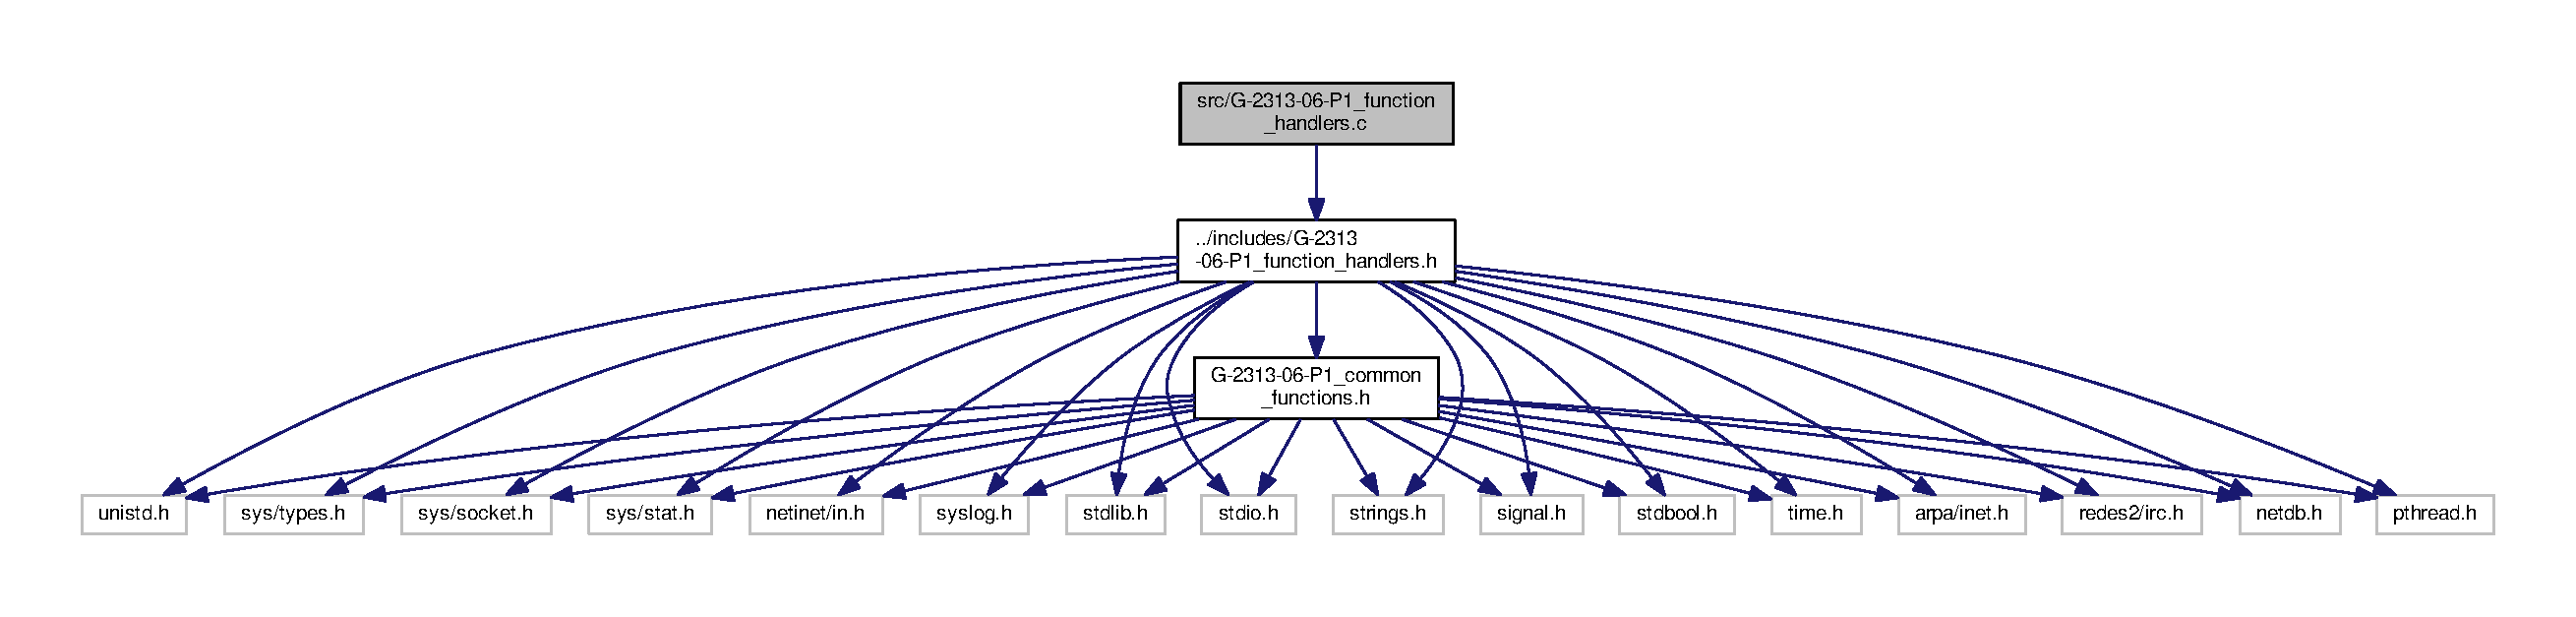
\includegraphics[width=350pt]{G-2313-06-P1__function__handlers_8c__incl}
\end{center}
\end{figure}
\subsection*{Funciones}
\begin{DoxyCompactItemize}
\item 
void \hyperlink{G-2313-06-P1__function__handlers_8c_aeefab469ba48ce1655dd5afd14f104b4}{server\+\_\+command\+\_\+nick} (char $\ast$command, int desc, char $\ast$nick\+\_\+static, int $\ast$register\+\_\+status)
\item 
void \hyperlink{G-2313-06-P1__function__handlers_8c_ad09156d6bd4cf58f4345e0bf851ff099}{server\+\_\+command\+\_\+user} (char $\ast$command, int desc, char $\ast$nick\+\_\+static, int $\ast$register\+\_\+status)
\item 
void \hyperlink{G-2313-06-P1__function__handlers_8c_a375c143c5469d1bb4fa7793b310ad68e}{server\+\_\+command\+\_\+join} (char $\ast$command, int desc, char $\ast$nick\+\_\+static, int $\ast$register\+\_\+status)
\item 
void \hyperlink{G-2313-06-P1__function__handlers_8c_a3df99a1f2cefc2d91d65cbb6dd555f96}{server\+\_\+command\+\_\+quit} (char $\ast$command, int desc, char $\ast$nick\+\_\+static, int $\ast$register\+\_\+status)
\item 
void \hyperlink{G-2313-06-P1__function__handlers_8c_acc1c181bf44087b9216d1b59809937aa}{server\+\_\+command\+\_\+ping} (char $\ast$command, int desc, char $\ast$nick\+\_\+static, int $\ast$register\+\_\+status)
\item 
void \hyperlink{G-2313-06-P1__function__handlers_8c_af289e3cc397e24e9b8c12c35bce68285}{server\+\_\+command\+\_\+list} (char $\ast$command, int desc, char $\ast$nick\+\_\+static, int $\ast$register\+\_\+status)
\item 
void \hyperlink{G-2313-06-P1__function__handlers_8c_a8daf68135f2d9e9412c04a2980bdfb2f}{server\+\_\+command\+\_\+privmsg} (char $\ast$command, int desc, char $\ast$nick\+\_\+static, int $\ast$register\+\_\+status)
\item 
void \hyperlink{G-2313-06-P1__function__handlers_8c_aba1a3da1fb58bb35076e7ea56037463e}{server\+\_\+command\+\_\+part} (char $\ast$command, int desc, char $\ast$nick\+\_\+static, int $\ast$register\+\_\+status)
\item 
void \hyperlink{G-2313-06-P1__function__handlers_8c_a0fe05d80af27ae220f8fa631468606ea}{server\+\_\+command\+\_\+names} (char $\ast$command, int desc, char $\ast$nick\+\_\+static, int $\ast$register\+\_\+status)
\item 
void \hyperlink{G-2313-06-P1__function__handlers_8c_a33025bd9c7bf8fbb2bf9cf722c07465c}{server\+\_\+command\+\_\+kick} (char $\ast$command, int desc, char $\ast$nick\+\_\+static, int $\ast$register\+\_\+status)
\item 
void \hyperlink{G-2313-06-P1__function__handlers_8c_a44a8736512c1df49d94c8194ae9b8a50}{server\+\_\+command\+\_\+mode} (char $\ast$command, int desc, char $\ast$nick\+\_\+static, int $\ast$register\+\_\+status)
\item 
void \hyperlink{G-2313-06-P1__function__handlers_8c_a327516a6c48e34b58428f7a502938928}{server\+\_\+command\+\_\+away} (char $\ast$command, int desc, char $\ast$nick\+\_\+static, int $\ast$register\+\_\+status)
\item 
void \hyperlink{G-2313-06-P1__function__handlers_8c_a8bb934f01707fcb12ebac41f1fe69441}{server\+\_\+command\+\_\+whois} (char $\ast$command, int desc, char $\ast$nick\+\_\+static, int $\ast$register\+\_\+status)
\item 
void \hyperlink{G-2313-06-P1__function__handlers_8c_a894ae019e03841e9d54fdad31d79f218}{server\+\_\+command\+\_\+topic} (char $\ast$command, int desc, char $\ast$nick\+\_\+static, int $\ast$register\+\_\+status)
\item 
void \hyperlink{G-2313-06-P1__function__handlers_8c_a1258d3bdf779b82c3f952bdde3d62631}{server\+\_\+command\+\_\+motd} (char $\ast$command, int desc, char $\ast$nick\+\_\+static, int $\ast$register\+\_\+status)
\end{DoxyCompactItemize}


\subsection{Documentación de las funciones}
\hypertarget{G-2313-06-P1__function__handlers_8c_a327516a6c48e34b58428f7a502938928}{}\index{G-\/2313-\/06-\/\+P1\+\_\+function\+\_\+handlers.\+c@{G-\/2313-\/06-\/\+P1\+\_\+function\+\_\+handlers.\+c}!server\+\_\+command\+\_\+away@{server\+\_\+command\+\_\+away}}
\index{server\+\_\+command\+\_\+away@{server\+\_\+command\+\_\+away}!G-\/2313-\/06-\/\+P1\+\_\+function\+\_\+handlers.\+c@{G-\/2313-\/06-\/\+P1\+\_\+function\+\_\+handlers.\+c}}
\subsubsection[{server\+\_\+command\+\_\+away}]{\setlength{\rightskip}{0pt plus 5cm}void server\+\_\+command\+\_\+away (
\begin{DoxyParamCaption}
\item[{char $\ast$}]{command, }
\item[{int}]{desc, }
\item[{char $\ast$}]{nick\+\_\+static, }
\item[{int $\ast$}]{register\+\_\+status}
\end{DoxyParamCaption}
)}\label{G-2313-06-P1__function__handlers_8c_a327516a6c48e34b58428f7a502938928}


Definición en la línea 1001 del archivo G-\/2313-\/06-\/\+P1\+\_\+function\+\_\+handlers.\+c.

\hypertarget{G-2313-06-P1__function__handlers_8c_a375c143c5469d1bb4fa7793b310ad68e}{}\index{G-\/2313-\/06-\/\+P1\+\_\+function\+\_\+handlers.\+c@{G-\/2313-\/06-\/\+P1\+\_\+function\+\_\+handlers.\+c}!server\+\_\+command\+\_\+join@{server\+\_\+command\+\_\+join}}
\index{server\+\_\+command\+\_\+join@{server\+\_\+command\+\_\+join}!G-\/2313-\/06-\/\+P1\+\_\+function\+\_\+handlers.\+c@{G-\/2313-\/06-\/\+P1\+\_\+function\+\_\+handlers.\+c}}
\subsubsection[{server\+\_\+command\+\_\+join}]{\setlength{\rightskip}{0pt plus 5cm}void server\+\_\+command\+\_\+join (
\begin{DoxyParamCaption}
\item[{char $\ast$}]{command, }
\item[{int}]{desc, }
\item[{char $\ast$}]{nick\+\_\+static, }
\item[{int $\ast$}]{register\+\_\+status}
\end{DoxyParamCaption}
)}\label{G-2313-06-P1__function__handlers_8c_a375c143c5469d1bb4fa7793b310ad68e}


Definición en la línea 255 del archivo G-\/2313-\/06-\/\+P1\+\_\+function\+\_\+handlers.\+c.

\hypertarget{G-2313-06-P1__function__handlers_8c_a33025bd9c7bf8fbb2bf9cf722c07465c}{}\index{G-\/2313-\/06-\/\+P1\+\_\+function\+\_\+handlers.\+c@{G-\/2313-\/06-\/\+P1\+\_\+function\+\_\+handlers.\+c}!server\+\_\+command\+\_\+kick@{server\+\_\+command\+\_\+kick}}
\index{server\+\_\+command\+\_\+kick@{server\+\_\+command\+\_\+kick}!G-\/2313-\/06-\/\+P1\+\_\+function\+\_\+handlers.\+c@{G-\/2313-\/06-\/\+P1\+\_\+function\+\_\+handlers.\+c}}
\subsubsection[{server\+\_\+command\+\_\+kick}]{\setlength{\rightskip}{0pt plus 5cm}void server\+\_\+command\+\_\+kick (
\begin{DoxyParamCaption}
\item[{char $\ast$}]{command, }
\item[{int}]{desc, }
\item[{char $\ast$}]{nick\+\_\+static, }
\item[{int $\ast$}]{register\+\_\+status}
\end{DoxyParamCaption}
)}\label{G-2313-06-P1__function__handlers_8c_a33025bd9c7bf8fbb2bf9cf722c07465c}


Definición en la línea 786 del archivo G-\/2313-\/06-\/\+P1\+\_\+function\+\_\+handlers.\+c.

\hypertarget{G-2313-06-P1__function__handlers_8c_af289e3cc397e24e9b8c12c35bce68285}{}\index{G-\/2313-\/06-\/\+P1\+\_\+function\+\_\+handlers.\+c@{G-\/2313-\/06-\/\+P1\+\_\+function\+\_\+handlers.\+c}!server\+\_\+command\+\_\+list@{server\+\_\+command\+\_\+list}}
\index{server\+\_\+command\+\_\+list@{server\+\_\+command\+\_\+list}!G-\/2313-\/06-\/\+P1\+\_\+function\+\_\+handlers.\+c@{G-\/2313-\/06-\/\+P1\+\_\+function\+\_\+handlers.\+c}}
\subsubsection[{server\+\_\+command\+\_\+list}]{\setlength{\rightskip}{0pt plus 5cm}void server\+\_\+command\+\_\+list (
\begin{DoxyParamCaption}
\item[{char $\ast$}]{command, }
\item[{int}]{desc, }
\item[{char $\ast$}]{nick\+\_\+static, }
\item[{int $\ast$}]{register\+\_\+status}
\end{DoxyParamCaption}
)}\label{G-2313-06-P1__function__handlers_8c_af289e3cc397e24e9b8c12c35bce68285}


Definición en la línea 472 del archivo G-\/2313-\/06-\/\+P1\+\_\+function\+\_\+handlers.\+c.

\hypertarget{G-2313-06-P1__function__handlers_8c_a44a8736512c1df49d94c8194ae9b8a50}{}\index{G-\/2313-\/06-\/\+P1\+\_\+function\+\_\+handlers.\+c@{G-\/2313-\/06-\/\+P1\+\_\+function\+\_\+handlers.\+c}!server\+\_\+command\+\_\+mode@{server\+\_\+command\+\_\+mode}}
\index{server\+\_\+command\+\_\+mode@{server\+\_\+command\+\_\+mode}!G-\/2313-\/06-\/\+P1\+\_\+function\+\_\+handlers.\+c@{G-\/2313-\/06-\/\+P1\+\_\+function\+\_\+handlers.\+c}}
\subsubsection[{server\+\_\+command\+\_\+mode}]{\setlength{\rightskip}{0pt plus 5cm}void server\+\_\+command\+\_\+mode (
\begin{DoxyParamCaption}
\item[{char $\ast$}]{command, }
\item[{int}]{desc, }
\item[{char $\ast$}]{nick\+\_\+static, }
\item[{int $\ast$}]{register\+\_\+status}
\end{DoxyParamCaption}
)}\label{G-2313-06-P1__function__handlers_8c_a44a8736512c1df49d94c8194ae9b8a50}


Definición en la línea 879 del archivo G-\/2313-\/06-\/\+P1\+\_\+function\+\_\+handlers.\+c.

\hypertarget{G-2313-06-P1__function__handlers_8c_a1258d3bdf779b82c3f952bdde3d62631}{}\index{G-\/2313-\/06-\/\+P1\+\_\+function\+\_\+handlers.\+c@{G-\/2313-\/06-\/\+P1\+\_\+function\+\_\+handlers.\+c}!server\+\_\+command\+\_\+motd@{server\+\_\+command\+\_\+motd}}
\index{server\+\_\+command\+\_\+motd@{server\+\_\+command\+\_\+motd}!G-\/2313-\/06-\/\+P1\+\_\+function\+\_\+handlers.\+c@{G-\/2313-\/06-\/\+P1\+\_\+function\+\_\+handlers.\+c}}
\subsubsection[{server\+\_\+command\+\_\+motd}]{\setlength{\rightskip}{0pt plus 5cm}void server\+\_\+command\+\_\+motd (
\begin{DoxyParamCaption}
\item[{char $\ast$}]{command, }
\item[{int}]{desc, }
\item[{char $\ast$}]{nick\+\_\+static, }
\item[{int $\ast$}]{register\+\_\+status}
\end{DoxyParamCaption}
)}\label{G-2313-06-P1__function__handlers_8c_a1258d3bdf779b82c3f952bdde3d62631}


Definición en la línea 1265 del archivo G-\/2313-\/06-\/\+P1\+\_\+function\+\_\+handlers.\+c.

\hypertarget{G-2313-06-P1__function__handlers_8c_a0fe05d80af27ae220f8fa631468606ea}{}\index{G-\/2313-\/06-\/\+P1\+\_\+function\+\_\+handlers.\+c@{G-\/2313-\/06-\/\+P1\+\_\+function\+\_\+handlers.\+c}!server\+\_\+command\+\_\+names@{server\+\_\+command\+\_\+names}}
\index{server\+\_\+command\+\_\+names@{server\+\_\+command\+\_\+names}!G-\/2313-\/06-\/\+P1\+\_\+function\+\_\+handlers.\+c@{G-\/2313-\/06-\/\+P1\+\_\+function\+\_\+handlers.\+c}}
\subsubsection[{server\+\_\+command\+\_\+names}]{\setlength{\rightskip}{0pt plus 5cm}void server\+\_\+command\+\_\+names (
\begin{DoxyParamCaption}
\item[{char $\ast$}]{command, }
\item[{int}]{desc, }
\item[{char $\ast$}]{nick\+\_\+static, }
\item[{int $\ast$}]{register\+\_\+status}
\end{DoxyParamCaption}
)}\label{G-2313-06-P1__function__handlers_8c_a0fe05d80af27ae220f8fa631468606ea}


Definición en la línea 711 del archivo G-\/2313-\/06-\/\+P1\+\_\+function\+\_\+handlers.\+c.

\hypertarget{G-2313-06-P1__function__handlers_8c_aeefab469ba48ce1655dd5afd14f104b4}{}\index{G-\/2313-\/06-\/\+P1\+\_\+function\+\_\+handlers.\+c@{G-\/2313-\/06-\/\+P1\+\_\+function\+\_\+handlers.\+c}!server\+\_\+command\+\_\+nick@{server\+\_\+command\+\_\+nick}}
\index{server\+\_\+command\+\_\+nick@{server\+\_\+command\+\_\+nick}!G-\/2313-\/06-\/\+P1\+\_\+function\+\_\+handlers.\+c@{G-\/2313-\/06-\/\+P1\+\_\+function\+\_\+handlers.\+c}}
\subsubsection[{server\+\_\+command\+\_\+nick}]{\setlength{\rightskip}{0pt plus 5cm}void server\+\_\+command\+\_\+nick (
\begin{DoxyParamCaption}
\item[{char $\ast$}]{command, }
\item[{int}]{desc, }
\item[{char $\ast$}]{nick\+\_\+static, }
\item[{int $\ast$}]{register\+\_\+status}
\end{DoxyParamCaption}
)}\label{G-2313-06-P1__function__handlers_8c_aeefab469ba48ce1655dd5afd14f104b4}


Definición en la línea 82 del archivo G-\/2313-\/06-\/\+P1\+\_\+function\+\_\+handlers.\+c.

\hypertarget{G-2313-06-P1__function__handlers_8c_aba1a3da1fb58bb35076e7ea56037463e}{}\index{G-\/2313-\/06-\/\+P1\+\_\+function\+\_\+handlers.\+c@{G-\/2313-\/06-\/\+P1\+\_\+function\+\_\+handlers.\+c}!server\+\_\+command\+\_\+part@{server\+\_\+command\+\_\+part}}
\index{server\+\_\+command\+\_\+part@{server\+\_\+command\+\_\+part}!G-\/2313-\/06-\/\+P1\+\_\+function\+\_\+handlers.\+c@{G-\/2313-\/06-\/\+P1\+\_\+function\+\_\+handlers.\+c}}
\subsubsection[{server\+\_\+command\+\_\+part}]{\setlength{\rightskip}{0pt plus 5cm}void server\+\_\+command\+\_\+part (
\begin{DoxyParamCaption}
\item[{char $\ast$}]{command, }
\item[{int}]{desc, }
\item[{char $\ast$}]{nick\+\_\+static, }
\item[{int $\ast$}]{register\+\_\+status}
\end{DoxyParamCaption}
)}\label{G-2313-06-P1__function__handlers_8c_aba1a3da1fb58bb35076e7ea56037463e}


Definición en la línea 644 del archivo G-\/2313-\/06-\/\+P1\+\_\+function\+\_\+handlers.\+c.

\hypertarget{G-2313-06-P1__function__handlers_8c_acc1c181bf44087b9216d1b59809937aa}{}\index{G-\/2313-\/06-\/\+P1\+\_\+function\+\_\+handlers.\+c@{G-\/2313-\/06-\/\+P1\+\_\+function\+\_\+handlers.\+c}!server\+\_\+command\+\_\+ping@{server\+\_\+command\+\_\+ping}}
\index{server\+\_\+command\+\_\+ping@{server\+\_\+command\+\_\+ping}!G-\/2313-\/06-\/\+P1\+\_\+function\+\_\+handlers.\+c@{G-\/2313-\/06-\/\+P1\+\_\+function\+\_\+handlers.\+c}}
\subsubsection[{server\+\_\+command\+\_\+ping}]{\setlength{\rightskip}{0pt plus 5cm}void server\+\_\+command\+\_\+ping (
\begin{DoxyParamCaption}
\item[{char $\ast$}]{command, }
\item[{int}]{desc, }
\item[{char $\ast$}]{nick\+\_\+static, }
\item[{int $\ast$}]{register\+\_\+status}
\end{DoxyParamCaption}
)}\label{G-2313-06-P1__function__handlers_8c_acc1c181bf44087b9216d1b59809937aa}


Definición en la línea 407 del archivo G-\/2313-\/06-\/\+P1\+\_\+function\+\_\+handlers.\+c.

\hypertarget{G-2313-06-P1__function__handlers_8c_a8daf68135f2d9e9412c04a2980bdfb2f}{}\index{G-\/2313-\/06-\/\+P1\+\_\+function\+\_\+handlers.\+c@{G-\/2313-\/06-\/\+P1\+\_\+function\+\_\+handlers.\+c}!server\+\_\+command\+\_\+privmsg@{server\+\_\+command\+\_\+privmsg}}
\index{server\+\_\+command\+\_\+privmsg@{server\+\_\+command\+\_\+privmsg}!G-\/2313-\/06-\/\+P1\+\_\+function\+\_\+handlers.\+c@{G-\/2313-\/06-\/\+P1\+\_\+function\+\_\+handlers.\+c}}
\subsubsection[{server\+\_\+command\+\_\+privmsg}]{\setlength{\rightskip}{0pt plus 5cm}void server\+\_\+command\+\_\+privmsg (
\begin{DoxyParamCaption}
\item[{char $\ast$}]{command, }
\item[{int}]{desc, }
\item[{char $\ast$}]{nick\+\_\+static, }
\item[{int $\ast$}]{register\+\_\+status}
\end{DoxyParamCaption}
)}\label{G-2313-06-P1__function__handlers_8c_a8daf68135f2d9e9412c04a2980bdfb2f}


Definición en la línea 542 del archivo G-\/2313-\/06-\/\+P1\+\_\+function\+\_\+handlers.\+c.

\hypertarget{G-2313-06-P1__function__handlers_8c_a3df99a1f2cefc2d91d65cbb6dd555f96}{}\index{G-\/2313-\/06-\/\+P1\+\_\+function\+\_\+handlers.\+c@{G-\/2313-\/06-\/\+P1\+\_\+function\+\_\+handlers.\+c}!server\+\_\+command\+\_\+quit@{server\+\_\+command\+\_\+quit}}
\index{server\+\_\+command\+\_\+quit@{server\+\_\+command\+\_\+quit}!G-\/2313-\/06-\/\+P1\+\_\+function\+\_\+handlers.\+c@{G-\/2313-\/06-\/\+P1\+\_\+function\+\_\+handlers.\+c}}
\subsubsection[{server\+\_\+command\+\_\+quit}]{\setlength{\rightskip}{0pt plus 5cm}void server\+\_\+command\+\_\+quit (
\begin{DoxyParamCaption}
\item[{char $\ast$}]{command, }
\item[{int}]{desc, }
\item[{char $\ast$}]{nick\+\_\+static, }
\item[{int $\ast$}]{register\+\_\+status}
\end{DoxyParamCaption}
)}\label{G-2313-06-P1__function__handlers_8c_a3df99a1f2cefc2d91d65cbb6dd555f96}


Definición en la línea 355 del archivo G-\/2313-\/06-\/\+P1\+\_\+function\+\_\+handlers.\+c.

\hypertarget{G-2313-06-P1__function__handlers_8c_a894ae019e03841e9d54fdad31d79f218}{}\index{G-\/2313-\/06-\/\+P1\+\_\+function\+\_\+handlers.\+c@{G-\/2313-\/06-\/\+P1\+\_\+function\+\_\+handlers.\+c}!server\+\_\+command\+\_\+topic@{server\+\_\+command\+\_\+topic}}
\index{server\+\_\+command\+\_\+topic@{server\+\_\+command\+\_\+topic}!G-\/2313-\/06-\/\+P1\+\_\+function\+\_\+handlers.\+c@{G-\/2313-\/06-\/\+P1\+\_\+function\+\_\+handlers.\+c}}
\subsubsection[{server\+\_\+command\+\_\+topic}]{\setlength{\rightskip}{0pt plus 5cm}void server\+\_\+command\+\_\+topic (
\begin{DoxyParamCaption}
\item[{char $\ast$}]{command, }
\item[{int}]{desc, }
\item[{char $\ast$}]{nick\+\_\+static, }
\item[{int $\ast$}]{register\+\_\+status}
\end{DoxyParamCaption}
)}\label{G-2313-06-P1__function__handlers_8c_a894ae019e03841e9d54fdad31d79f218}


Definición en la línea 1186 del archivo G-\/2313-\/06-\/\+P1\+\_\+function\+\_\+handlers.\+c.

\hypertarget{G-2313-06-P1__function__handlers_8c_ad09156d6bd4cf58f4345e0bf851ff099}{}\index{G-\/2313-\/06-\/\+P1\+\_\+function\+\_\+handlers.\+c@{G-\/2313-\/06-\/\+P1\+\_\+function\+\_\+handlers.\+c}!server\+\_\+command\+\_\+user@{server\+\_\+command\+\_\+user}}
\index{server\+\_\+command\+\_\+user@{server\+\_\+command\+\_\+user}!G-\/2313-\/06-\/\+P1\+\_\+function\+\_\+handlers.\+c@{G-\/2313-\/06-\/\+P1\+\_\+function\+\_\+handlers.\+c}}
\subsubsection[{server\+\_\+command\+\_\+user}]{\setlength{\rightskip}{0pt plus 5cm}void server\+\_\+command\+\_\+user (
\begin{DoxyParamCaption}
\item[{char $\ast$}]{command, }
\item[{int}]{desc, }
\item[{char $\ast$}]{nick\+\_\+static, }
\item[{int $\ast$}]{register\+\_\+status}
\end{DoxyParamCaption}
)}\label{G-2313-06-P1__function__handlers_8c_ad09156d6bd4cf58f4345e0bf851ff099}


Definición en la línea 179 del archivo G-\/2313-\/06-\/\+P1\+\_\+function\+\_\+handlers.\+c.

\hypertarget{G-2313-06-P1__function__handlers_8c_a8bb934f01707fcb12ebac41f1fe69441}{}\index{G-\/2313-\/06-\/\+P1\+\_\+function\+\_\+handlers.\+c@{G-\/2313-\/06-\/\+P1\+\_\+function\+\_\+handlers.\+c}!server\+\_\+command\+\_\+whois@{server\+\_\+command\+\_\+whois}}
\index{server\+\_\+command\+\_\+whois@{server\+\_\+command\+\_\+whois}!G-\/2313-\/06-\/\+P1\+\_\+function\+\_\+handlers.\+c@{G-\/2313-\/06-\/\+P1\+\_\+function\+\_\+handlers.\+c}}
\subsubsection[{server\+\_\+command\+\_\+whois}]{\setlength{\rightskip}{0pt plus 5cm}void server\+\_\+command\+\_\+whois (
\begin{DoxyParamCaption}
\item[{char $\ast$}]{command, }
\item[{int}]{desc, }
\item[{char $\ast$}]{nick\+\_\+static, }
\item[{int $\ast$}]{register\+\_\+status}
\end{DoxyParamCaption}
)}\label{G-2313-06-P1__function__handlers_8c_a8bb934f01707fcb12ebac41f1fe69441}


Definición en la línea 1061 del archivo G-\/2313-\/06-\/\+P1\+\_\+function\+\_\+handlers.\+c.


\hypertarget{G-2313-06-P1__server_8c}{}\section{Referencia del Archivo src/\+G-\/2313-\/06-\/\+P1\+\_\+server.c}
\label{G-2313-06-P1__server_8c}\index{src/\+G-\/2313-\/06-\/\+P1\+\_\+server.\+c@{src/\+G-\/2313-\/06-\/\+P1\+\_\+server.\+c}}
{\ttfamily \#include \char`\"{}../includes/\+G-\/2313-\/06-\/\+P1\+\_\+server.\+h\char`\"{}}\\*
Dependencia gráfica adjunta para G-\/2313-\/06-\/\+P1\+\_\+server.c\+:\nopagebreak
\begin{figure}[H]
\begin{center}
\leavevmode
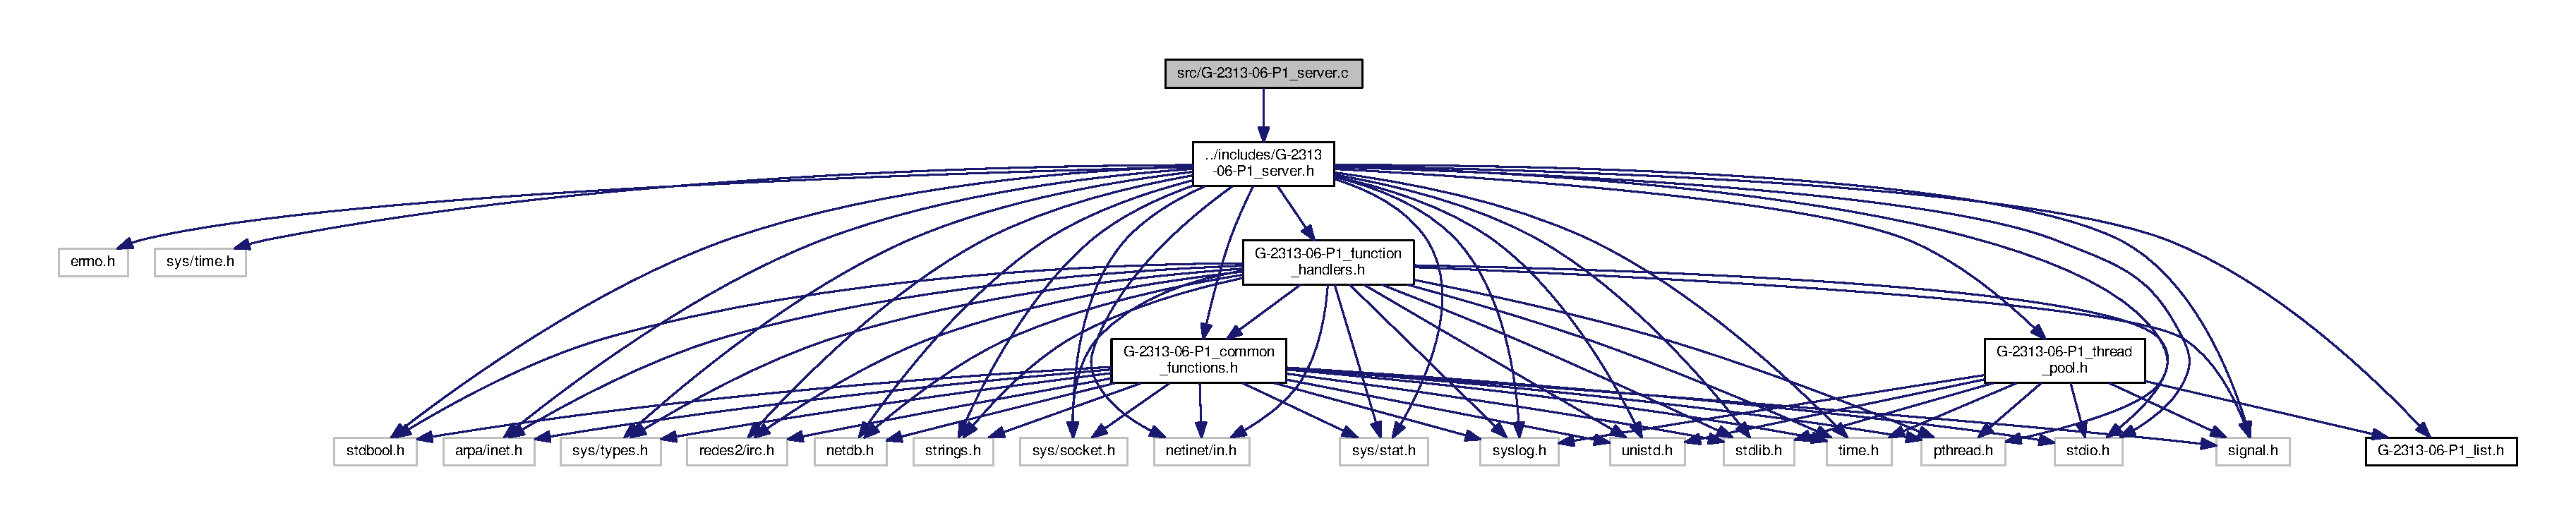
\includegraphics[width=350pt]{G-2313-06-P1__server_8c__incl}
\end{center}
\end{figure}
\subsection*{Funciones}
\begin{DoxyCompactItemize}
\item 
int \hyperlink{G-2313-06-P1__server_8c_aa8cae03a9b52c7a550cbbdcc8aa74ede}{server\+\_\+start} ()
\item 
void \hyperlink{G-2313-06-P1__server_8c_aaac8642d2e699e0f9d942d28a9b233c2}{server\+\_\+accept\+\_\+connection} (int socket\+\_\+desc)
\item 
void $\ast$ \hyperlink{G-2313-06-P1__server_8c_a81394df6131e7cf998bd06f63f9e3995}{server\+\_\+start\+\_\+communication} (int socket\+\_\+desc)
\item 
void \hyperlink{G-2313-06-P1__server_8c_a775161328c3264fb8f96981f7a9c83ae}{server\+\_\+execute\+\_\+function} (long function\+Name, char $\ast$command, int desc, char $\ast$nick, int $\ast$register\+\_\+status)
\item 
void \hyperlink{G-2313-06-P1__server_8c_a0e947005d451a8f3bf3af01f54b59f11}{server\+\_\+exit} ()
\item 
int \hyperlink{G-2313-06-P1__server_8c_a64f1fffc5903ccf0350845cd21a95b6e}{server\+\_\+check\+\_\+socket\+\_\+status} (int socket\+\_\+desc)
\item 
void \hyperlink{G-2313-06-P1__server_8c_aa0e8000b12d9c52fc1e87847d00c9c47}{server\+\_\+daemon} ()
\item 
void \hyperlink{G-2313-06-P1__server_8c_a48d522cd984dc64ecd084f05416b1a94}{server\+\_\+start\+\_\+pool} ()
\item 
int \hyperlink{G-2313-06-P1__server_8c_ae66f6b31b5ad750f1fe042a706a4e3d4}{main} ()
\end{DoxyCompactItemize}
\subsection*{Variables}
\begin{DoxyCompactItemize}
\item 
\hyperlink{structthread__pool__t}{thread\+\_\+pool\+\_\+t} $\ast$ \hyperlink{G-2313-06-P1__server_8c_a57d8a6a060b67bdc5946cd0e7331575a}{pool} = N\+U\+L\+L
\end{DoxyCompactItemize}


\subsection{Documentación de las funciones}
\hypertarget{G-2313-06-P1__server_8c_ae66f6b31b5ad750f1fe042a706a4e3d4}{}\index{G-\/2313-\/06-\/\+P1\+\_\+server.\+c@{G-\/2313-\/06-\/\+P1\+\_\+server.\+c}!main@{main}}
\index{main@{main}!G-\/2313-\/06-\/\+P1\+\_\+server.\+c@{G-\/2313-\/06-\/\+P1\+\_\+server.\+c}}
\subsubsection[{main}]{\setlength{\rightskip}{0pt plus 5cm}int main (
\begin{DoxyParamCaption}
{}
\end{DoxyParamCaption}
)}\label{G-2313-06-P1__server_8c_ae66f6b31b5ad750f1fe042a706a4e3d4}


Definición en la línea 565 del archivo G-\/2313-\/06-\/\+P1\+\_\+server.\+c.

\hypertarget{G-2313-06-P1__server_8c_aaac8642d2e699e0f9d942d28a9b233c2}{}\index{G-\/2313-\/06-\/\+P1\+\_\+server.\+c@{G-\/2313-\/06-\/\+P1\+\_\+server.\+c}!server\+\_\+accept\+\_\+connection@{server\+\_\+accept\+\_\+connection}}
\index{server\+\_\+accept\+\_\+connection@{server\+\_\+accept\+\_\+connection}!G-\/2313-\/06-\/\+P1\+\_\+server.\+c@{G-\/2313-\/06-\/\+P1\+\_\+server.\+c}}
\subsubsection[{server\+\_\+accept\+\_\+connection}]{\setlength{\rightskip}{0pt plus 5cm}void server\+\_\+accept\+\_\+connection (
\begin{DoxyParamCaption}
\item[{int}]{socket\+\_\+desc}
\end{DoxyParamCaption}
)}\label{G-2313-06-P1__server_8c_aaac8642d2e699e0f9d942d28a9b233c2}


Definición en la línea 171 del archivo G-\/2313-\/06-\/\+P1\+\_\+server.\+c.

\hypertarget{G-2313-06-P1__server_8c_a64f1fffc5903ccf0350845cd21a95b6e}{}\index{G-\/2313-\/06-\/\+P1\+\_\+server.\+c@{G-\/2313-\/06-\/\+P1\+\_\+server.\+c}!server\+\_\+check\+\_\+socket\+\_\+status@{server\+\_\+check\+\_\+socket\+\_\+status}}
\index{server\+\_\+check\+\_\+socket\+\_\+status@{server\+\_\+check\+\_\+socket\+\_\+status}!G-\/2313-\/06-\/\+P1\+\_\+server.\+c@{G-\/2313-\/06-\/\+P1\+\_\+server.\+c}}
\subsubsection[{server\+\_\+check\+\_\+socket\+\_\+status}]{\setlength{\rightskip}{0pt plus 5cm}int server\+\_\+check\+\_\+socket\+\_\+status (
\begin{DoxyParamCaption}
\item[{int}]{socket\+\_\+desc}
\end{DoxyParamCaption}
)}\label{G-2313-06-P1__server_8c_a64f1fffc5903ccf0350845cd21a95b6e}


Definición en la línea 473 del archivo G-\/2313-\/06-\/\+P1\+\_\+server.\+c.

\hypertarget{G-2313-06-P1__server_8c_aa0e8000b12d9c52fc1e87847d00c9c47}{}\index{G-\/2313-\/06-\/\+P1\+\_\+server.\+c@{G-\/2313-\/06-\/\+P1\+\_\+server.\+c}!server\+\_\+daemon@{server\+\_\+daemon}}
\index{server\+\_\+daemon@{server\+\_\+daemon}!G-\/2313-\/06-\/\+P1\+\_\+server.\+c@{G-\/2313-\/06-\/\+P1\+\_\+server.\+c}}
\subsubsection[{server\+\_\+daemon}]{\setlength{\rightskip}{0pt plus 5cm}void server\+\_\+daemon (
\begin{DoxyParamCaption}
{}
\end{DoxyParamCaption}
)}\label{G-2313-06-P1__server_8c_aa0e8000b12d9c52fc1e87847d00c9c47}


Definición en la línea 518 del archivo G-\/2313-\/06-\/\+P1\+\_\+server.\+c.

\hypertarget{G-2313-06-P1__server_8c_a775161328c3264fb8f96981f7a9c83ae}{}\index{G-\/2313-\/06-\/\+P1\+\_\+server.\+c@{G-\/2313-\/06-\/\+P1\+\_\+server.\+c}!server\+\_\+execute\+\_\+function@{server\+\_\+execute\+\_\+function}}
\index{server\+\_\+execute\+\_\+function@{server\+\_\+execute\+\_\+function}!G-\/2313-\/06-\/\+P1\+\_\+server.\+c@{G-\/2313-\/06-\/\+P1\+\_\+server.\+c}}
\subsubsection[{server\+\_\+execute\+\_\+function}]{\setlength{\rightskip}{0pt plus 5cm}void server\+\_\+execute\+\_\+function (
\begin{DoxyParamCaption}
\item[{long}]{function\+Name, }
\item[{char $\ast$}]{command, }
\item[{int}]{desc, }
\item[{char $\ast$}]{nick, }
\item[{int $\ast$}]{register\+\_\+status}
\end{DoxyParamCaption}
)}\label{G-2313-06-P1__server_8c_a775161328c3264fb8f96981f7a9c83ae}


Definición en la línea 368 del archivo G-\/2313-\/06-\/\+P1\+\_\+server.\+c.

\hypertarget{G-2313-06-P1__server_8c_a0e947005d451a8f3bf3af01f54b59f11}{}\index{G-\/2313-\/06-\/\+P1\+\_\+server.\+c@{G-\/2313-\/06-\/\+P1\+\_\+server.\+c}!server\+\_\+exit@{server\+\_\+exit}}
\index{server\+\_\+exit@{server\+\_\+exit}!G-\/2313-\/06-\/\+P1\+\_\+server.\+c@{G-\/2313-\/06-\/\+P1\+\_\+server.\+c}}
\subsubsection[{server\+\_\+exit}]{\setlength{\rightskip}{0pt plus 5cm}void server\+\_\+exit (
\begin{DoxyParamCaption}
{}
\end{DoxyParamCaption}
)}\label{G-2313-06-P1__server_8c_a0e947005d451a8f3bf3af01f54b59f11}


Definición en la línea 436 del archivo G-\/2313-\/06-\/\+P1\+\_\+server.\+c.

\hypertarget{G-2313-06-P1__server_8c_aa8cae03a9b52c7a550cbbdcc8aa74ede}{}\index{G-\/2313-\/06-\/\+P1\+\_\+server.\+c@{G-\/2313-\/06-\/\+P1\+\_\+server.\+c}!server\+\_\+start@{server\+\_\+start}}
\index{server\+\_\+start@{server\+\_\+start}!G-\/2313-\/06-\/\+P1\+\_\+server.\+c@{G-\/2313-\/06-\/\+P1\+\_\+server.\+c}}
\subsubsection[{server\+\_\+start}]{\setlength{\rightskip}{0pt plus 5cm}int server\+\_\+start (
\begin{DoxyParamCaption}
\item[{void}]{}
\end{DoxyParamCaption}
)}\label{G-2313-06-P1__server_8c_aa8cae03a9b52c7a550cbbdcc8aa74ede}


Definición en la línea 101 del archivo G-\/2313-\/06-\/\+P1\+\_\+server.\+c.

\hypertarget{G-2313-06-P1__server_8c_a81394df6131e7cf998bd06f63f9e3995}{}\index{G-\/2313-\/06-\/\+P1\+\_\+server.\+c@{G-\/2313-\/06-\/\+P1\+\_\+server.\+c}!server\+\_\+start\+\_\+communication@{server\+\_\+start\+\_\+communication}}
\index{server\+\_\+start\+\_\+communication@{server\+\_\+start\+\_\+communication}!G-\/2313-\/06-\/\+P1\+\_\+server.\+c@{G-\/2313-\/06-\/\+P1\+\_\+server.\+c}}
\subsubsection[{server\+\_\+start\+\_\+communication}]{\setlength{\rightskip}{0pt plus 5cm}void$\ast$ server\+\_\+start\+\_\+communication (
\begin{DoxyParamCaption}
\item[{int}]{socket\+\_\+desc}
\end{DoxyParamCaption}
)}\label{G-2313-06-P1__server_8c_a81394df6131e7cf998bd06f63f9e3995}


Definición en la línea 252 del archivo G-\/2313-\/06-\/\+P1\+\_\+server.\+c.

\hypertarget{G-2313-06-P1__server_8c_a48d522cd984dc64ecd084f05416b1a94}{}\index{G-\/2313-\/06-\/\+P1\+\_\+server.\+c@{G-\/2313-\/06-\/\+P1\+\_\+server.\+c}!server\+\_\+start\+\_\+pool@{server\+\_\+start\+\_\+pool}}
\index{server\+\_\+start\+\_\+pool@{server\+\_\+start\+\_\+pool}!G-\/2313-\/06-\/\+P1\+\_\+server.\+c@{G-\/2313-\/06-\/\+P1\+\_\+server.\+c}}
\subsubsection[{server\+\_\+start\+\_\+pool}]{\setlength{\rightskip}{0pt plus 5cm}void server\+\_\+start\+\_\+pool (
\begin{DoxyParamCaption}
{}
\end{DoxyParamCaption}
)}\label{G-2313-06-P1__server_8c_a48d522cd984dc64ecd084f05416b1a94}


Definición en la línea 558 del archivo G-\/2313-\/06-\/\+P1\+\_\+server.\+c.



\subsection{Documentación de las variables}
\hypertarget{G-2313-06-P1__server_8c_a57d8a6a060b67bdc5946cd0e7331575a}{}\index{G-\/2313-\/06-\/\+P1\+\_\+server.\+c@{G-\/2313-\/06-\/\+P1\+\_\+server.\+c}!pool@{pool}}
\index{pool@{pool}!G-\/2313-\/06-\/\+P1\+\_\+server.\+c@{G-\/2313-\/06-\/\+P1\+\_\+server.\+c}}
\subsubsection[{pool}]{\setlength{\rightskip}{0pt plus 5cm}{\bf thread\+\_\+pool\+\_\+t}$\ast$ pool = N\+U\+L\+L}\label{G-2313-06-P1__server_8c_a57d8a6a060b67bdc5946cd0e7331575a}


Definición en la línea 51 del archivo G-\/2313-\/06-\/\+P1\+\_\+server.\+c.


\hypertarget{G-2313-06-P1__thread__pool_8c}{}\section{Referencia del Archivo src/\+G-\/2313-\/06-\/\+P1\+\_\+thread\+\_\+pool.c}
\label{G-2313-06-P1__thread__pool_8c}\index{src/\+G-\/2313-\/06-\/\+P1\+\_\+thread\+\_\+pool.\+c@{src/\+G-\/2313-\/06-\/\+P1\+\_\+thread\+\_\+pool.\+c}}
{\ttfamily \#include \char`\"{}../includes/\+G-\/2313-\/06-\/\+P1\+\_\+thread\+\_\+pool.\+h\char`\"{}}\\*
Dependencia gráfica adjunta para G-\/2313-\/06-\/\+P1\+\_\+thread\+\_\+pool.c\+:
% FIG 0
\subsection*{Funciones}
\begin{DoxyCompactItemize}
\item 
\hyperlink{structthread__pool__t}{thread\+\_\+pool\+\_\+t} $\ast$ \hyperlink{G-2313-06-P1__thread__pool_8c_ae4c7364510f378011559c4eb6078e3ea}{thread\+\_\+pool\+\_\+create} (int size)
\item 
void \hyperlink{G-2313-06-P1__thread__pool_8c_a46b14e66a9466a68fa4f67a2e08e81fd}{thread\+\_\+pool\+\_\+delete} (\hyperlink{structthread__pool__t}{thread\+\_\+pool\+\_\+t} $\ast$p)
\item 
int \hyperlink{G-2313-06-P1__thread__pool_8c_a46e84068eca615afa66b5544ea7a2518}{thread\+\_\+pool\+\_\+init} (\hyperlink{structthread__pool__t}{thread\+\_\+pool\+\_\+t} $\ast$p)
\item 
int \hyperlink{G-2313-06-P1__thread__pool_8c_ae2a8c98f4f014e5b9d632bb678d7127a}{thread\+\_\+pool\+\_\+init\+\_\+internal} (\hyperlink{structthread__pool__t}{thread\+\_\+pool\+\_\+t} $\ast$p, double low\+\_\+level, double high\+\_\+level, int master\+\_\+interval)
\item 
\hyperlink{structthread__t}{thread\+\_\+t} $\ast$ \hyperlink{G-2313-06-P1__thread__pool_8c_a920e51bce81dfc069372dd87935db55e}{thread\+\_\+create} (void)
\item 
int \hyperlink{G-2313-06-P1__thread__pool_8c_a9aa2b7b210972e06e1a7d0775ba520b3}{thread\+\_\+add} (\hyperlink{structthread__pool__t}{thread\+\_\+pool\+\_\+t} $\ast$p, \hyperlink{structthread__t}{thread\+\_\+t} $\ast$t)
\item 
void \hyperlink{G-2313-06-P1__thread__pool_8c_a95970a6ee2f49963fc3fe7aefa677194}{thread\+\_\+del} (\hyperlink{structthread__t}{thread\+\_\+t} $\ast$t)
\item 
void \hyperlink{G-2313-06-P1__thread__pool_8c_a1fe4c198a9a46014fbac70eb443018a1}{thread\+\_\+del\+\_\+internal} (\hyperlink{structthread__pool__t}{thread\+\_\+pool\+\_\+t} $\ast$p, \hyperlink{structthread__t}{thread\+\_\+t} $\ast$t, int force\+\_\+lock)
\item 
void $\ast$ \hyperlink{G-2313-06-P1__thread__pool_8c_a4ef081fb21acd34e0e2492a9f290b6a3}{worker\+\_\+callback} (void $\ast$arg)
\item 
void $\ast$ \hyperlink{G-2313-06-P1__thread__pool_8c_a54703c23462be974a5e2511247921922}{master\+\_\+callback} (void $\ast$arg)
\item 
\hyperlink{structtask__t}{task\+\_\+t} $\ast$ \hyperlink{G-2313-06-P1__thread__pool_8c_afa05870619a7e753d41b8135b8514a2c}{task\+\_\+create} (void)
\item 
void \hyperlink{G-2313-06-P1__thread__pool_8c_a5665a923c48ff85abd630ddf83eb9999}{task\+\_\+init} (\hyperlink{structtask__t}{task\+\_\+t} $\ast$t, void $\ast$($\ast$task\+\_\+callback)(int), int arg)
\item 
void \hyperlink{G-2313-06-P1__thread__pool_8c_a90a0cb9adb9500b4f205edd942fc8272}{task\+\_\+add} (\hyperlink{structthread__pool__t}{thread\+\_\+pool\+\_\+t} $\ast$p, \hyperlink{structtask__t}{task\+\_\+t} $\ast$t)
\end{DoxyCompactItemize}


\subsection{Documentación de las funciones}
\index{G-\/2313-\/06-\/\+P1\+\_\+thread\+\_\+pool.\+c@{G-\/2313-\/06-\/\+P1\+\_\+thread\+\_\+pool.\+c}!master\+\_\+callback@{master\+\_\+callback}}
\index{master\+\_\+callback@{master\+\_\+callback}!G-\/2313-\/06-\/\+P1\+\_\+thread\+\_\+pool.\+c@{G-\/2313-\/06-\/\+P1\+\_\+thread\+\_\+pool.\+c}}
\subsubsection[{\texorpdfstring{master\+\_\+callback(void $\ast$arg)}{master_callback(void *arg)}}]{\setlength{\rightskip}{0pt plus 5cm}void$\ast$ master\+\_\+callback (
\begin{DoxyParamCaption}
\item[{void $\ast$}]{arg}
\end{DoxyParamCaption}
)}\hypertarget{G-2313-06-P1__thread__pool_8c_a54703c23462be974a5e2511247921922}{}\label{G-2313-06-P1__thread__pool_8c_a54703c23462be974a5e2511247921922}


Definición en la línea 222 del archivo G-\/2313-\/06-\/\+P1\+\_\+thread\+\_\+pool.\+c.

\index{G-\/2313-\/06-\/\+P1\+\_\+thread\+\_\+pool.\+c@{G-\/2313-\/06-\/\+P1\+\_\+thread\+\_\+pool.\+c}!task\+\_\+add@{task\+\_\+add}}
\index{task\+\_\+add@{task\+\_\+add}!G-\/2313-\/06-\/\+P1\+\_\+thread\+\_\+pool.\+c@{G-\/2313-\/06-\/\+P1\+\_\+thread\+\_\+pool.\+c}}
\subsubsection[{\texorpdfstring{task\+\_\+add(thread\+\_\+pool\+\_\+t $\ast$p, task\+\_\+t $\ast$t)}{task_add(thread_pool_t *p, task_t *t)}}]{\setlength{\rightskip}{0pt plus 5cm}void task\+\_\+add (
\begin{DoxyParamCaption}
\item[{{\bf thread\+\_\+pool\+\_\+t} $\ast$}]{p, }
\item[{{\bf task\+\_\+t} $\ast$}]{t}
\end{DoxyParamCaption}
)}\hypertarget{G-2313-06-P1__thread__pool_8c_a90a0cb9adb9500b4f205edd942fc8272}{}\label{G-2313-06-P1__thread__pool_8c_a90a0cb9adb9500b4f205edd942fc8272}


Definición en la línea 277 del archivo G-\/2313-\/06-\/\+P1\+\_\+thread\+\_\+pool.\+c.

\index{G-\/2313-\/06-\/\+P1\+\_\+thread\+\_\+pool.\+c@{G-\/2313-\/06-\/\+P1\+\_\+thread\+\_\+pool.\+c}!task\+\_\+create@{task\+\_\+create}}
\index{task\+\_\+create@{task\+\_\+create}!G-\/2313-\/06-\/\+P1\+\_\+thread\+\_\+pool.\+c@{G-\/2313-\/06-\/\+P1\+\_\+thread\+\_\+pool.\+c}}
\subsubsection[{\texorpdfstring{task\+\_\+create(void)}{task_create(void)}}]{\setlength{\rightskip}{0pt plus 5cm}{\bf task\+\_\+t}$\ast$ task\+\_\+create (
\begin{DoxyParamCaption}
\item[{void}]{}
\end{DoxyParamCaption}
)}\hypertarget{G-2313-06-P1__thread__pool_8c_afa05870619a7e753d41b8135b8514a2c}{}\label{G-2313-06-P1__thread__pool_8c_afa05870619a7e753d41b8135b8514a2c}


Definición en la línea 259 del archivo G-\/2313-\/06-\/\+P1\+\_\+thread\+\_\+pool.\+c.

\index{G-\/2313-\/06-\/\+P1\+\_\+thread\+\_\+pool.\+c@{G-\/2313-\/06-\/\+P1\+\_\+thread\+\_\+pool.\+c}!task\+\_\+init@{task\+\_\+init}}
\index{task\+\_\+init@{task\+\_\+init}!G-\/2313-\/06-\/\+P1\+\_\+thread\+\_\+pool.\+c@{G-\/2313-\/06-\/\+P1\+\_\+thread\+\_\+pool.\+c}}
\subsubsection[{\texorpdfstring{task\+\_\+init(task\+\_\+t $\ast$t, void $\ast$($\ast$task\+\_\+callback)(int), int arg)}{task_init(task_t *t, void *(*task_callback)(int), int arg)}}]{\setlength{\rightskip}{0pt plus 5cm}void task\+\_\+init (
\begin{DoxyParamCaption}
\item[{{\bf task\+\_\+t} $\ast$}]{t, }
\item[{void $\ast$($\ast$)(int)}]{task\+\_\+callback, }
\item[{int}]{arg}
\end{DoxyParamCaption}
)}\hypertarget{G-2313-06-P1__thread__pool_8c_a5665a923c48ff85abd630ddf83eb9999}{}\label{G-2313-06-P1__thread__pool_8c_a5665a923c48ff85abd630ddf83eb9999}


Definición en la línea 271 del archivo G-\/2313-\/06-\/\+P1\+\_\+thread\+\_\+pool.\+c.

\index{G-\/2313-\/06-\/\+P1\+\_\+thread\+\_\+pool.\+c@{G-\/2313-\/06-\/\+P1\+\_\+thread\+\_\+pool.\+c}!thread\+\_\+add@{thread\+\_\+add}}
\index{thread\+\_\+add@{thread\+\_\+add}!G-\/2313-\/06-\/\+P1\+\_\+thread\+\_\+pool.\+c@{G-\/2313-\/06-\/\+P1\+\_\+thread\+\_\+pool.\+c}}
\subsubsection[{\texorpdfstring{thread\+\_\+add(thread\+\_\+pool\+\_\+t $\ast$p, thread\+\_\+t $\ast$t)}{thread_add(thread_pool_t *p, thread_t *t)}}]{\setlength{\rightskip}{0pt plus 5cm}int thread\+\_\+add (
\begin{DoxyParamCaption}
\item[{{\bf thread\+\_\+pool\+\_\+t} $\ast$}]{p, }
\item[{{\bf thread\+\_\+t} $\ast$}]{t}
\end{DoxyParamCaption}
)}\hypertarget{G-2313-06-P1__thread__pool_8c_a9aa2b7b210972e06e1a7d0775ba520b3}{}\label{G-2313-06-P1__thread__pool_8c_a9aa2b7b210972e06e1a7d0775ba520b3}


Definición en la línea 121 del archivo G-\/2313-\/06-\/\+P1\+\_\+thread\+\_\+pool.\+c.

\index{G-\/2313-\/06-\/\+P1\+\_\+thread\+\_\+pool.\+c@{G-\/2313-\/06-\/\+P1\+\_\+thread\+\_\+pool.\+c}!thread\+\_\+create@{thread\+\_\+create}}
\index{thread\+\_\+create@{thread\+\_\+create}!G-\/2313-\/06-\/\+P1\+\_\+thread\+\_\+pool.\+c@{G-\/2313-\/06-\/\+P1\+\_\+thread\+\_\+pool.\+c}}
\subsubsection[{\texorpdfstring{thread\+\_\+create(void)}{thread_create(void)}}]{\setlength{\rightskip}{0pt plus 5cm}{\bf thread\+\_\+t}$\ast$ thread\+\_\+create (
\begin{DoxyParamCaption}
\item[{void}]{}
\end{DoxyParamCaption}
)}\hypertarget{G-2313-06-P1__thread__pool_8c_a920e51bce81dfc069372dd87935db55e}{}\label{G-2313-06-P1__thread__pool_8c_a920e51bce81dfc069372dd87935db55e}


Definición en la línea 109 del archivo G-\/2313-\/06-\/\+P1\+\_\+thread\+\_\+pool.\+c.

\index{G-\/2313-\/06-\/\+P1\+\_\+thread\+\_\+pool.\+c@{G-\/2313-\/06-\/\+P1\+\_\+thread\+\_\+pool.\+c}!thread\+\_\+del@{thread\+\_\+del}}
\index{thread\+\_\+del@{thread\+\_\+del}!G-\/2313-\/06-\/\+P1\+\_\+thread\+\_\+pool.\+c@{G-\/2313-\/06-\/\+P1\+\_\+thread\+\_\+pool.\+c}}
\subsubsection[{\texorpdfstring{thread\+\_\+del(thread\+\_\+t $\ast$t)}{thread_del(thread_t *t)}}]{\setlength{\rightskip}{0pt plus 5cm}void thread\+\_\+del (
\begin{DoxyParamCaption}
\item[{{\bf thread\+\_\+t} $\ast$}]{t}
\end{DoxyParamCaption}
)}\hypertarget{G-2313-06-P1__thread__pool_8c_a95970a6ee2f49963fc3fe7aefa677194}{}\label{G-2313-06-P1__thread__pool_8c_a95970a6ee2f49963fc3fe7aefa677194}


Definición en la línea 152 del archivo G-\/2313-\/06-\/\+P1\+\_\+thread\+\_\+pool.\+c.

\index{G-\/2313-\/06-\/\+P1\+\_\+thread\+\_\+pool.\+c@{G-\/2313-\/06-\/\+P1\+\_\+thread\+\_\+pool.\+c}!thread\+\_\+del\+\_\+internal@{thread\+\_\+del\+\_\+internal}}
\index{thread\+\_\+del\+\_\+internal@{thread\+\_\+del\+\_\+internal}!G-\/2313-\/06-\/\+P1\+\_\+thread\+\_\+pool.\+c@{G-\/2313-\/06-\/\+P1\+\_\+thread\+\_\+pool.\+c}}
\subsubsection[{\texorpdfstring{thread\+\_\+del\+\_\+internal(thread\+\_\+pool\+\_\+t $\ast$p, thread\+\_\+t $\ast$t, int force\+\_\+lock)}{thread_del_internal(thread_pool_t *p, thread_t *t, int force_lock)}}]{\setlength{\rightskip}{0pt plus 5cm}void thread\+\_\+del\+\_\+internal (
\begin{DoxyParamCaption}
\item[{{\bf thread\+\_\+pool\+\_\+t} $\ast$}]{p, }
\item[{{\bf thread\+\_\+t} $\ast$}]{t, }
\item[{int}]{force\+\_\+lock}
\end{DoxyParamCaption}
)}\hypertarget{G-2313-06-P1__thread__pool_8c_a1fe4c198a9a46014fbac70eb443018a1}{}\label{G-2313-06-P1__thread__pool_8c_a1fe4c198a9a46014fbac70eb443018a1}


Definición en la línea 159 del archivo G-\/2313-\/06-\/\+P1\+\_\+thread\+\_\+pool.\+c.

\index{G-\/2313-\/06-\/\+P1\+\_\+thread\+\_\+pool.\+c@{G-\/2313-\/06-\/\+P1\+\_\+thread\+\_\+pool.\+c}!thread\+\_\+pool\+\_\+create@{thread\+\_\+pool\+\_\+create}}
\index{thread\+\_\+pool\+\_\+create@{thread\+\_\+pool\+\_\+create}!G-\/2313-\/06-\/\+P1\+\_\+thread\+\_\+pool.\+c@{G-\/2313-\/06-\/\+P1\+\_\+thread\+\_\+pool.\+c}}
\subsubsection[{\texorpdfstring{thread\+\_\+pool\+\_\+create(int size)}{thread_pool_create(int size)}}]{\setlength{\rightskip}{0pt plus 5cm}{\bf thread\+\_\+pool\+\_\+t}$\ast$ thread\+\_\+pool\+\_\+create (
\begin{DoxyParamCaption}
\item[{int}]{size}
\end{DoxyParamCaption}
)}\hypertarget{G-2313-06-P1__thread__pool_8c_ae4c7364510f378011559c4eb6078e3ea}{}\label{G-2313-06-P1__thread__pool_8c_ae4c7364510f378011559c4eb6078e3ea}


Definición en la línea 3 del archivo G-\/2313-\/06-\/\+P1\+\_\+thread\+\_\+pool.\+c.

\index{G-\/2313-\/06-\/\+P1\+\_\+thread\+\_\+pool.\+c@{G-\/2313-\/06-\/\+P1\+\_\+thread\+\_\+pool.\+c}!thread\+\_\+pool\+\_\+delete@{thread\+\_\+pool\+\_\+delete}}
\index{thread\+\_\+pool\+\_\+delete@{thread\+\_\+pool\+\_\+delete}!G-\/2313-\/06-\/\+P1\+\_\+thread\+\_\+pool.\+c@{G-\/2313-\/06-\/\+P1\+\_\+thread\+\_\+pool.\+c}}
\subsubsection[{\texorpdfstring{thread\+\_\+pool\+\_\+delete(thread\+\_\+pool\+\_\+t $\ast$p)}{thread_pool_delete(thread_pool_t *p)}}]{\setlength{\rightskip}{0pt plus 5cm}void thread\+\_\+pool\+\_\+delete (
\begin{DoxyParamCaption}
\item[{{\bf thread\+\_\+pool\+\_\+t} $\ast$}]{p}
\end{DoxyParamCaption}
)}\hypertarget{G-2313-06-P1__thread__pool_8c_a46b14e66a9466a68fa4f67a2e08e81fd}{}\label{G-2313-06-P1__thread__pool_8c_a46b14e66a9466a68fa4f67a2e08e81fd}


Definición en la línea 27 del archivo G-\/2313-\/06-\/\+P1\+\_\+thread\+\_\+pool.\+c.

\index{G-\/2313-\/06-\/\+P1\+\_\+thread\+\_\+pool.\+c@{G-\/2313-\/06-\/\+P1\+\_\+thread\+\_\+pool.\+c}!thread\+\_\+pool\+\_\+init@{thread\+\_\+pool\+\_\+init}}
\index{thread\+\_\+pool\+\_\+init@{thread\+\_\+pool\+\_\+init}!G-\/2313-\/06-\/\+P1\+\_\+thread\+\_\+pool.\+c@{G-\/2313-\/06-\/\+P1\+\_\+thread\+\_\+pool.\+c}}
\subsubsection[{\texorpdfstring{thread\+\_\+pool\+\_\+init(thread\+\_\+pool\+\_\+t $\ast$p)}{thread_pool_init(thread_pool_t *p)}}]{\setlength{\rightskip}{0pt plus 5cm}int thread\+\_\+pool\+\_\+init (
\begin{DoxyParamCaption}
\item[{{\bf thread\+\_\+pool\+\_\+t} $\ast$}]{p}
\end{DoxyParamCaption}
)}\hypertarget{G-2313-06-P1__thread__pool_8c_a46e84068eca615afa66b5544ea7a2518}{}\label{G-2313-06-P1__thread__pool_8c_a46e84068eca615afa66b5544ea7a2518}


Definición en la línea 58 del archivo G-\/2313-\/06-\/\+P1\+\_\+thread\+\_\+pool.\+c.

\index{G-\/2313-\/06-\/\+P1\+\_\+thread\+\_\+pool.\+c@{G-\/2313-\/06-\/\+P1\+\_\+thread\+\_\+pool.\+c}!thread\+\_\+pool\+\_\+init\+\_\+internal@{thread\+\_\+pool\+\_\+init\+\_\+internal}}
\index{thread\+\_\+pool\+\_\+init\+\_\+internal@{thread\+\_\+pool\+\_\+init\+\_\+internal}!G-\/2313-\/06-\/\+P1\+\_\+thread\+\_\+pool.\+c@{G-\/2313-\/06-\/\+P1\+\_\+thread\+\_\+pool.\+c}}
\subsubsection[{\texorpdfstring{thread\+\_\+pool\+\_\+init\+\_\+internal(thread\+\_\+pool\+\_\+t $\ast$p, double low\+\_\+level, double high\+\_\+level, int master\+\_\+interval)}{thread_pool_init_internal(thread_pool_t *p, double low_level, double high_level, int master_interval)}}]{\setlength{\rightskip}{0pt plus 5cm}int thread\+\_\+pool\+\_\+init\+\_\+internal (
\begin{DoxyParamCaption}
\item[{{\bf thread\+\_\+pool\+\_\+t} $\ast$}]{p, }
\item[{double}]{low\+\_\+level, }
\item[{double}]{high\+\_\+level, }
\item[{int}]{master\+\_\+interval}
\end{DoxyParamCaption}
)}\hypertarget{G-2313-06-P1__thread__pool_8c_ae2a8c98f4f014e5b9d632bb678d7127a}{}\label{G-2313-06-P1__thread__pool_8c_ae2a8c98f4f014e5b9d632bb678d7127a}


Definición en la línea 64 del archivo G-\/2313-\/06-\/\+P1\+\_\+thread\+\_\+pool.\+c.

\index{G-\/2313-\/06-\/\+P1\+\_\+thread\+\_\+pool.\+c@{G-\/2313-\/06-\/\+P1\+\_\+thread\+\_\+pool.\+c}!worker\+\_\+callback@{worker\+\_\+callback}}
\index{worker\+\_\+callback@{worker\+\_\+callback}!G-\/2313-\/06-\/\+P1\+\_\+thread\+\_\+pool.\+c@{G-\/2313-\/06-\/\+P1\+\_\+thread\+\_\+pool.\+c}}
\subsubsection[{\texorpdfstring{worker\+\_\+callback(void $\ast$arg)}{worker_callback(void *arg)}}]{\setlength{\rightskip}{0pt plus 5cm}void$\ast$ worker\+\_\+callback (
\begin{DoxyParamCaption}
\item[{void $\ast$}]{arg}
\end{DoxyParamCaption}
)}\hypertarget{G-2313-06-P1__thread__pool_8c_a4ef081fb21acd34e0e2492a9f290b6a3}{}\label{G-2313-06-P1__thread__pool_8c_a4ef081fb21acd34e0e2492a9f290b6a3}


Definición en la línea 171 del archivo G-\/2313-\/06-\/\+P1\+\_\+thread\+\_\+pool.\+c.


%--- End generated contents ---

% Index
\backmatter
\newpage
\phantomsection
\clearemptydoublepage
\addcontentsline{toc}{chapter}{Índice}
\printindex

\end{document}
